%%%%%%%%%%%%%
%%%%%%%%%%%%%
%
% preamble
%
%%%%%%%%%%%%
%%%%%%%%%%%%

\documentclass[11pt]{amsart}

% load packages

\usepackage{amsfonts, amsthm, amssymb, amsmath, stmaryrd, etoolbox}
\usepackage{comment}
\usepackage{mathtools}
\usepackage{graphicx,caption,subcaption}
\usepackage{todonotes}
\usepackage{xcolor}

\usepackage[inline]{enumitem}
\setlist{itemsep=0em, topsep=0em, parsep=0em}
\setlist[enumerate]{label=(\alph*)}

\usepackage{tikz}
\usepackage[all,2cell]{xy}
\usepackage[all,2cell]{xy}
\usetikzlibrary{matrix,arrows,shapes,decorations.markings,decorations.pathreplacing}
\tikzset{rewritenode/.style={shape=circle,draw,minimum size=1em}}
\tikzset{RWopen/.style={shape=circle,draw=black,fill=white,scale=0.5,font=\Huge}}
\tikzset{RWclosed/.style={shape=circle,fill=black,scale=0.5,font=\Huge}}
\tikzset{CDnode/.style={shape=circle,fill=white,scale=.5}}
\tikzset{->-/.style={decoration={markings,mark=at position .5 with {\arrow{>}}},postaction={decorate}}}

\usepackage{hyperref}
\definecolor{hyperrefcolor}{rgb}{0,0,0.7}
\hypersetup{colorlinks,linkcolor={hyperrefcolor},citecolor={hyperrefcolor},urlcolor={hyperrefcolor}}

% new commands

\newcommand{\RR}{\mathbb{R}}
\newcommand{\ZZ}{\mathbb{Z}}
\newcommand{\NN}{\mathbb{N}}
\newcommand{\QQ}{\mathbb{Q}}
\newcommand{\CC}{\mathbb{C}}
\renewcommand{\epsilon}{\varepsilon}

\newcommand{\cl}[1]{\mathcal{#1}}
\newcommand{\scr}[1]{\mathscr{#1}}
\newcommand{\op}[1]{\operatorname{#1}}
\newcommand{\cat}[1]{\mathbf{#1}}
\newcommand{\dblcat}[1]{\mathbb{#1}}
\renewcommand{\t}[1]{\textup{#1}}

\newcommand{\from}{\colon}
\newcommand{\xto}[1]{\xrightarrow{#1}}
\newcommand{\sm}{\smallsetminus}
\newcommand{\tospan}{\xrightarrow{\mathit{sp}}}
\newcommand{\tocospan}{\xrightarrow{\mathit{csp}}}

%\newcommand{\diagram}[1]{\raisebox{-0.5\height}{\includegraphics{#1}}}

\newcommand{\bluebullet}{\textcolor{rewritecolor}{\bullet}}

%  macros for (co)span bicategories
\newcommand{\bispmap}[1]{\mathbf{Sp(#1)}}
\newcommand{\dblspmap}[1]{\mathbb{S}\mathbf{p(#1)}}
\newcommand{\bicspmap}[1]{\mathbf{Csp(#1)}}
\newcommand{\dblcspmap}[1]{\mathbb{C}\mathbf{sp(#1)}}
\newcommand{\bispsp}[1]{\mathbf{Sp(Sp(#1))}}
\newcommand{\dblspsp}[1]{\mathbb{S}\mathbf{p(Sp(#1))}}
\newcommand{\bicspcsp}[1]{\mathbf{Csp(Csp(#1))}}
\newcommand{\dblcspcsp}[1]{\mathbb{C}\mathbf{sp(Csp(#1))}}
\newcommand{\bimonspcsp}[1]{\mathbf{MonicSp(Csp(#1))}}
\newcommand{\dblmonspcsp}[1]{\mathbb{M}\mathbf{onicSp(Csp(#1))}}
\newcommand{\biepiccspsp}[1]{\mathbf{EpicCsp(Sp(#1))}}
\newcommand{\dblepiccspsp}[1]{\mathbb{E}\mathbf{picCsp(Sp(#1))}}

% defining arrow with a vertical line through it
\makeatletter
\def\slashedarrowfill@#1#2#3#4#5{%
	$\m@th\thickmuskip0mu\medmuskip\thickmuskip\thinmuskip\thickmuskip
	\relax#5#1\mkern-7mu%
	\cleaders\hbox{$#5\mkern-2mu#2\mkern-2mu$}\hfill
	\mathclap{#3}\mathclap{#2}%
	\cleaders\hbox{$#5\mkern-2mu#2\mkern-2mu$}\hfill
	\mkern-7mu#4$%
}
\def\rightslashedarrowfill@{%
	\slashedarrowfill@\relbar\relbar\mapstochar\rightarrow}
\newcommand{\xslashedrightarrow}[2][]{%
	\ext@arrow 0055{\rightslashedarrowfill@}{#1}{#2}}
\makeatother

\newcommand{\hto}{\xslashedrightarrow{}}


% declare math operators

\DeclareMathOperator{\Hom}{Hom}
\DeclareMathOperator{\id}{id}
\DeclareMathOperator{\ob}{Ob}
\DeclareMathOperator{\arr}{arr}
\DeclareMathOperator{\im}{im}
\DeclareMathOperator{\Aut}{Aut}
\DeclareMathOperator{\Bij}{Bij}
\DeclareMathOperator{\Sub}{Sub}

% environments and counters

\newtheorem{thm}{Theorem}[section]
\newtheorem{lem}[thm]{Lemma}
\newtheorem{prop}[thm]{Proposition}
\newtheorem{cor}[thm]{Corollary}

\theoremstyle{remark}
\newtheorem{remark}[thm]{Remark}
\newtheorem{notation}[thm]{Notation}

\theoremstyle{definition}
\newtheorem{ex}[thm]{Example} 
\newtheorem{defn}[thm]{Definition}

%\setcounter{tocdepth}{1} % Sets depth for table of contents. 

%%%%%%%%%%
%%%%%%%%%%
%%%%%%%%%%
%%%%%%%%%%
%
% begin documnet
%
%%%%%%%%%%
%%%%%%%%%%
%%%%%%%%%%
%%%%%%%%%%

\begin{document}
\sloppy	
%\tableofcontents

\begin{abstract}
If $\cat{C}$ is a category with chosen pullbacks and a terminal object, then using a result of Shulman, we show how to obtain a symmetric monoidal bicategory $\cat{Sp(Sp(C))}$ with objects being those of $\cat{C}$, morphisms as spans in $\cat{C}$ and 2-morphisms as isomorphism classes of spans of spans of $\cat{C}$. We also show that this bicategory is fully dualizable. Moreover, if $\cat{C}$ has properties resembling those of a topos, Cicala has shown that there is a bicategory $\cat{MonicSp(Csp(C))}$ with objects being those of $\cat{C}$, morphisms as cospans in $\cat{C}$ and 2-morphisms as isomorphism classes of spans of cospans in $\cat{C}$ where the morphisms of the inner span are monomorphisms. Here we show this bicategory is also symmetric monoidal and even compact closed. Applications of such bicategories can be seen in graph rewriting rules as well as in Morton and Vicary's combinatorial approach to Khovanov's categorified Heisenberg algebra.
\end{abstract}

\title{Bicategories of Spans and Cospans}
\author{Daniel Cicala \and Kenny Courser}
\maketitle

%%%%%%%%%%
%%%%%%%%%%
\section{Introduction} 
\label{sec:Introduction}
%%%%%%%%%%
%%%%%%%%%%

Given a category $\cat{C}$ with finite limits, various categories and bicategories involving spans in $\cat{C}$ can be constructed and such constructions go back to B\'enabou \cite{Be} in what was one of the first examples of a bicategory. Since then, many others, not exclusive to Courser, Rebro and Stay \cite{Cour,Reb,Stay} have proven many related results. In this paper, we investigate properties of three types of cospan bicategories whose differences lie in the $2$-morphisms.  The three different sorts of $2$-morphisms are maps of cospans, cospans of cospans, and monic spans of cospans.  These $2$-morphisms are compared in Figure \ref{fig:2cells}. 


\begin{figure}[h]
	\centering
	\begin{tabular}{|ccc|}
		% Row 1
		\hline
		{$2$-morphisms} & bicategory & double category \\
		% Row 2
		\hline \hline 
		{Maps of Spans} & 
		% Maps of spans bicategory
		$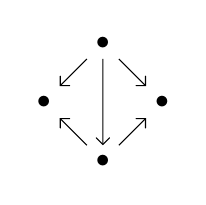
\begin{tikzpicture}[baseline=(current bounding box.center),scale=0.75]
		\node (A) at (0,0) {$\bullet$};
		\node (B) at (1,1) {$\bullet$};
		\node (B') at (1,-1) {$\bullet$};
		\node (C) at (2,0) {$\bullet$};
		%
		\path[->,font=\scriptsize,>=angle 90]
		(B) edge node[above]{} (A)
		(B') edge node[above]{} (A)
		(B) edge node[above]{} (C)
		(B') edge node[above]{} (C)
		(B) edge node[left]{} (B');
		\end{tikzpicture}$ &
		% Maps of spans double category
		$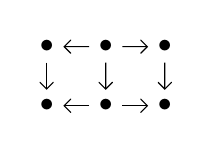
\begin{tikzpicture}[baseline=(current bounding box.center),scale=0.75]
		\node (A) at (0,1) {$\bullet$};
		\node (A') at (0,0) {$\bullet$};
		\node (B) at (1,1) {$\bullet$};
		\node (B') at (1,0) {$\bullet$};
		\node (C) at (2,1) {$\bullet$};
		\node (C') at (2,0) {$\bullet$};
		%
		\path[->,font=\scriptsize,>=angle 90]
		% horizontal arrows
		(B) edge node[above]{} (A)
		(B) edge node[above]{} (C)
		(B') edge node[above]{} (A')
		(B') edge node[above]{} (C')
		% vertical arrows
		(A) edge node[left]{} (A')
		(B) edge node[left]{} (B')
		(C) edge node[left]{} (C');	
		\end{tikzpicture}$ \\
		% Row 3
		\hline 
		{Maps of Cospans} &
		% maps of cospans bicategory
		$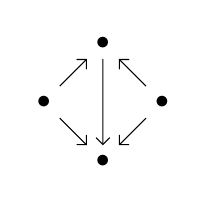
\begin{tikzpicture}[baseline=(current bounding box.center),scale=0.75]
		\node (A) at (0,0) {$\bullet$};
		\node (B) at (1,1) {$\bullet$};
		\node (B') at (1,-1) {$\bullet$};
		\node (C) at (2,0) {$\bullet$};
		%
		\path[->,font=\scriptsize,>=angle 90]
		(A) edge node[above]{} (B)
		(A) edge node[above]{} (B')
		(C) edge node[above]{} (B)
		(C) edge node[above]{} (B')
		(B) edge node[left]{} (B');
		\end{tikzpicture}$ &
		% maps of cospans double category
		$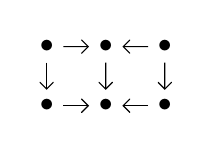
\begin{tikzpicture}[baseline=(current bounding box.center),scale=0.75]
		\node (A) at (0,1) {$\bullet$};
		\node (A') at (0,0) {$\bullet$};
		\node (B) at (1,1) {$\bullet$};
		\node (B') at (1,0) {$\bullet$};
		\node (C) at (2,1) {$\bullet$};
		\node (C') at (2,0) {$\bullet$};
		%
		\path[->,font=\scriptsize,>=angle 90]
		% horizontal arrows
		(A) edge node[above]{} (B)
		(C) edge node[above]{} (B)
		(A') edge node[above]{} (B')
		(C') edge node[above]{} (B')
		% vertical arrows
		(A) edge node[left]{} (A')
		(B) edge node[left]{} (B')
		(C) edge node[left]{} (C');	
		\end{tikzpicture}$\\
		% Row 4
		\hline 
		{Spans of Spans} & 
		% spans of spans bicategory
		$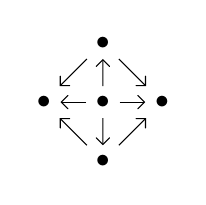
\begin{tikzpicture}[baseline=(current bounding box.center),scale=0.75]
		\node (A) at (0,0) {$\bullet$};
		\node (B) at (1,1) {$\bullet$};
		\node (B') at (1,0) {$\bullet$};
		\node (B'') at (1,-1) {$\bullet$};
		\node (C) at (2,0) {$\bullet$};
		%
		\path[->,font=\scriptsize,>=angle 90]
		(B) edge node[above]{} (A)
		(B) edge node[above]{} (C)
		(B') edge[->] node[left]{} (A)
		(B') edge[->] node[right]{} (C)
		(B'') edge node[left]{} (A)
		(B'') edge node[left]{} (C)
		(B') edge node[left]{} (B)
		(B') edge node[right]{} (B'');
		\end{tikzpicture}$ &
		% spans of spans double category
		$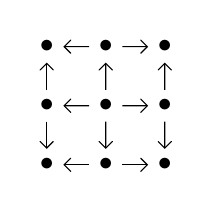
\begin{tikzpicture}[baseline=(current bounding box.center),scale=0.75]
		\node (A) at (0,2) {$\bullet$};
		\node (A') at (0,1) {$\bullet$};
		\node (A'') at (0,0) {$\bullet$};
		\node (B) at (1,2) {$\bullet$};
		\node (B') at (1,1) {$\bullet$};
		\node (B'') at (1,0) {$\bullet$};
		\node (C) at (2,2) {$\bullet$};
		\node (C') at (2,1) {$\bullet$};
		\node (C'') at (2,0) {$\bullet$};
		%
		\path[->,font=\scriptsize,>=angle 90]
		% horizontal arrows
		(B) edge node[above]{} (A)
		(B) edge node[above]{} (C)
		(B') edge node[above]{} (A')
		(B') edge node[above]{} (C')
		(B'') edge node[above]{} (A'')
		(B'') edge node[above]{} (C'')
		% vertical arrows
		(A') edge node[left]{} (A)
		(A') edge node[left]{} (A'')
		(B') edge node[left]{} (B)
		(B') edge node[left]{} (B'')
		(C') edge node[left]{} (C)
		(C') edge node[left]{} (C'');	
		\end{tikzpicture}$\\
		% Row 5
		\hline 
		{Cospans of Copans} & 
		% cospans of cospans bicategory
		$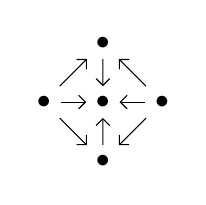
\begin{tikzpicture}[baseline=(current bounding box.center),scale=0.75]
		\node (A) at (0,0) {$\bullet$};
		\node (B) at (1,1) {$\bullet$};
		\node (B') at (1,0) {$\bullet$};
		\node (B'') at (1,-1) {$\bullet$};
		\node (C) at (2,0) {$\bullet$};
		%
		\path[->,font=\scriptsize,>=angle 90]
		(A) edge node[above]{} (B)
		(A) edge node[above]{} (B')
		(A) edge[->] node[left]{} (B'')
		(C) edge[->] node[right]{} (B)
		(C) edge node[left]{} (B')
		(C) edge node[left]{} (B'')
		(B) edge node[left]{} (B')
		(B'') edge node[right]{} (B');
		\end{tikzpicture}$ &
		% cospans of cospans double category
		$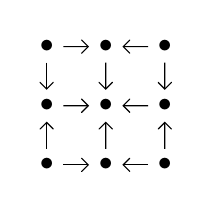
\begin{tikzpicture}[baseline=(current bounding box.center),scale=0.75]
		\node (A) at (0,2) {$\bullet$};
		\node (A') at (0,1) {$\bullet$};
		\node (A'') at (0,0) {$\bullet$};
		\node (B) at (1,2) {$\bullet$};
		\node (B') at (1,1) {$\bullet$};
		\node (B'') at (1,0) {$\bullet$};
		\node (C) at (2,2) {$\bullet$};
		\node (C') at (2,1) {$\bullet$};
		\node (C'') at (2,0) {$\bullet$};
		%
		\path[->,font=\scriptsize,>=angle 90]
		% horizontal arrows
		(A) edge node[above]{} (B)
		(A') edge node[above]{} (B')
		(A'') edge node[above]{} (B'')
		(C) edge node[above]{} (B)
		(C') edge node[above]{} (B')
		(C'') edge node[above]{} (B'')
		% vertical arrows
		(A) edge node[left]{} (A')
		(A'') edge node[left]{} (A')
		(B) edge node[left]{} (B')
		(B'') edge node[left]{} (B')
		(C) edge node[left]{} (C')
		(C'') edge node[left]{} (C');	
		\end{tikzpicture}$ \\
		% Row 6
		\hline 
		{Monic Spans of Copans} & 
		% monic spans of cospans bicategory
		$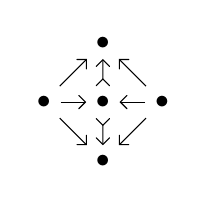
\begin{tikzpicture}[baseline=(current bounding box.center),scale=0.75]
		\node (A) at (0,0) {$\bullet$};
		\node (B) at (1,1) {$\bullet$};
		\node (B') at (1,0) {$\bullet$};
		\node (B'') at (1,-1) {$\bullet$};
		\node (C) at (2,0) {$\bullet$};
		%
		\path[->,font=\scriptsize,>=angle 90]
		(A) edge node[above]{$ $} (B)
		(A) edge node[above]{$ $} (B')
		(A) edge node[above]{$ $} (B'')
		(C) edge node[above]{$ $} (B)
		(C) edge node[above]{$ $} (B')
		(C) edge node[left]{$ $} (B'')
		(B') edge[>->] node[right]{$ $} (B)
		(B') edge[>->] node[left]{$ $} (B'');
		\end{tikzpicture}$ &
		% monic spans of cospans double category
		$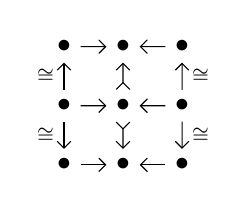
\begin{tikzpicture}[baseline=(current bounding box.center),scale=0.75]
		\node (A) at (0,2) {$\bullet$};
		\node (A') at (0,1) {$\bullet$};
		\node (A'') at (0,0) {$\bullet$};
		\node (B) at (1,2) {$\bullet$};
		\node (B') at (1,1) {$\bullet$};
		\node (B'') at (1,0) {$\bullet$};
		\node (C) at (2,2) {$\bullet$};
		\node (C') at (2,1) {$\bullet$};
		\node (C'') at (2,0) {$\bullet$};
		%
		\path[->,font=\scriptsize,>=angle 90]
		% horizontal arrows
		(A) edge node[above]{$ $} (B)
		(A') edge node[above]{$ $} (B')
		(A'') edge node[above]{$ $} (B'')
		(C) edge node[above]{$ $} (B)
		(C') edge node[above]{$ $} (B')
		(C'') edge node[above]{$ $} (B'')
		% vertical arrows
		(A') edge node[left]{$\cong$} (A)
		(A') edge node[left]{$\cong$} (A'')
		(B') edge[>->] node[left]{$ $} (B)
		(B') edge[>->] node[left]{$ $} (B'')
		(C') edge node[right]{$\cong$} (C)
		(C') edge node[right]{$\cong$} (C'');
		\end{tikzpicture}$ \\
		% Row 7
		\hline 
		{Epic Cospans of Spans} & 
		% epic cospans of spans bicategory
		$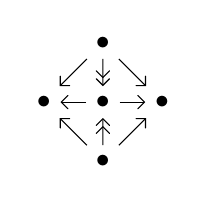
\begin{tikzpicture}[baseline=(current bounding box.center),scale=0.75]
		\node (A) at (0,0) {$\bullet$};
		\node (B) at (1,1) {$\bullet$};
		\node (B') at (1,0) {$\bullet$};
		\node (B'') at (1,-1) {$\bullet$};
		\node (C) at (2,0) {$\bullet$};
		%
		\path[->,font=\scriptsize,>=angle 90]
		(B) edge node[above]{$ $} (A)
		(B) edge node[left]{$ $} (C)
		(B') edge node[left]{$ $} (A)
		(B') edge node[right]{$ $} (C)
		(B'') edge node[left]{$ $} (A)
		(B'') edge node[left]{$ $} (C)
		(B) edge[->>] node[left]{$ $} (B')
		(B'') edge[->>] node[right]{$ $} (B');
		\end{tikzpicture}$ &
		% epic cospans of spans double category
		$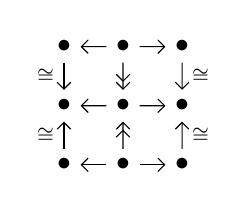
\begin{tikzpicture}[baseline=(current bounding box.center),scale=0.75]
		\node (A) at (0,2) {$\bullet$};
		\node (A') at (0,1) {$\bullet$};
		\node (A'') at (0,0) {$\bullet$};
		\node (B) at (1,2) {$\bullet$};
		\node (B') at (1,1) {$\bullet$};
		\node (B'') at (1,0) {$\bullet$};
		\node (C) at (2,2) {$\bullet$};;
		\node (C') at (2,1) {$\bullet$};
		\node (C'') at (2,0) {$\bullet$};
		%
		\path[->,font=\scriptsize,>=angle 90]
		% horizontal arrows
		(B) edge node[above]{$ $} (A)
		(B) edge node[above]{$ $} (C)
		(B') edge node[above]{$ $} (A')
		(B') edge node[above]{$ $} (C')
		(B'') edge node[above]{$ $} (A'')
		(B'') edge node[above]{$ $} (C'')
		% vertical arrows
		(A) edge node[left]{$\cong$} (A')
		(A'') edge node[left]{$\cong$} (A')
		(B) edge[->>] node[left]{$ $} (B')
		(B'') edge[->>] node[left]{$ $} (B')
		(C) edge node[right]{$\cong$} (C')
		(C'') edge node[right]{$\cong$} (C');
		\end{tikzpicture}$ \\
		\hline 
	\end{tabular}
	\caption{Bicategory and double category $2$-morphisms}
	\label{fig:2cells}
\end{figure}

One of the first examples of a bicategory, given by B\'enabou \cite{Be} in his landmark paper, consisted of objects, spans as morphisms and maps of spans as $2$-morphisms. It follows from dualizing work of Courser \cite{Cour} that this bicategory is symmetric monoidal. A map of spans can be seen as a special case of a span of spans with one of the legs as an identity. Here, using a result of Shulman \cite{Shul} that yields a symmetric monoidal bicategory from an isofibrant symmetric monoidal double category, we show that if $\cat{C}$ has chosen pullbacks and a terminal object, then there is a fully dualizable symmetric monoidal bicategory $\cat{Sp(Sp(C))}$ with
\begin{enumerate}
\item{objects of $\cat{C}$ as objects,}
\item{spans in $\cat{C}$ as morphisms, and}
\item{isomorphism classes of spans of spans in $\cat{C}$ as $2$-morphisms.}
\end{enumerate}

Morton and Vicary \cite{MortVic} have conjectured the existence of a symmetric monoidal bicategory with
\begin{enumerate}
\item{groupoids as objects,}
\item{spans of groupoids as morphisms which are composed via `weak pullbacks', also known as `iso-comma objects', and}
\item{isomorphism classes of spans of spans of groupoids as $2$-morphisms.}
\end{enumerate}
While we have not shown the existence of such a bicategory, we present an alternative construction whose idea is due to Steve Lack. Namely, given a functor $F \colon \hat{G} \to G$ between groupoids, one can replace the domain $\hat{G}$ with an equivalent groupoid $G^\prime$, and the functor $F$ with an `equivalent' functor $F^\prime \colon G^\prime \to G$ which happens to be a fibration \cite{Anderson,Bousfield,Strickland}. Using the equivalence $e \colon \hat{G} \to G^\prime$, we get a natural isomorphism $F \Rightarrow F^\prime e$. Moreover, given a cospan of groupoids, weak pullbacks and strict pullbacks are equivalent when one of the legs of the cospan is a fibration \cite{JoyalStreet1}, and moreover, fibrations are preserved by pullbacks \cite{Brown,Heath}. Thanks to these ideas, we show how to obtain a symmetric monoidal bicategory $\cat{Sp(Sp(\widehat{Gpd}))}$ consisting of groupoids, spans of groupoids whose legs are fibrations and isomorphism classes of spans of spans of groupoids in which all the morphisms are fibrations. We conjecture that this bicategory is biequivalent to the one used in the work of Morton and Vicary.

In a previous work, Cicala \cite{Cic} has combined the ideas of using spans or cospans as morphisms in a bicategory to create a bicategory that has cospans as morphisms and appropriate isomorphism classes of spans as $2$-morphisms. Namely, if $\cat{C}$ is a category with properties similar to those of a topos, he has shown that there exists a bicategory consisting of objects of $\cat{C}$, morphisms as cospans of $\cat{C}$, and $2$-morphisms as isomorphism classes of spans of cospans where the morphisms of the inner span are required to be monomorphisms as depicted in Figure \ref{fig:2cells}. We denote this bicategory as $\cat{MonicSp(Csp(C))}$. One might wonder whether the condition of the inner span being monic is necessary and if a more aesthetic result is possible, but Cicala has shown that this monic condition on the spans is indeed necessary. Again, using a result of Shulman, we show that $\cat{MonicSp(Csp(C))}$ is in fact symmetric monoidal by first constructing an appropriate isofibrant symmetric monoidal double category. Furthermore, we show that the symmetric monoidal bicategory $\cat{MonicSp(Csp(C))}$ is compact closed.

The primary motivation for constructing $\bimonspcsp{C}$ is the case where $\cat{C}$ is the topos $\cat{Graph}$ of directed graphs. There is a symmetric monoidal and compact closed sub-bicategory $\cat{Rewrite}$ that was introduced in \cite{Cic}. This is the full sub-bicategory of $\bimonspcsp{Graph}$ with edgeless graphs for objects.  The morphisms are graphs with inputs and outputs chosen by the feet of the cospans.  An example of such a morphism is a cospan of graphs
\[
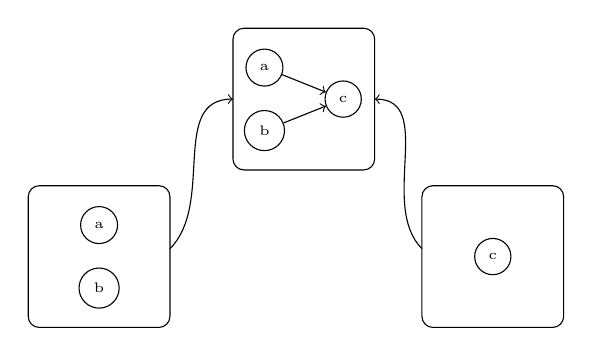
\begin{tikzpicture}[scale=1]
	\draw[rounded corners] (-0.8,1.6) rectangle (1,3.4);
	\draw[rounded corners] (4.2,1.6) rectangle (6,3.4);
	\draw[rounded corners] (1.8,3.6) rectangle (3.6,5.4);
	%
	\node[circle,draw] (ai) at (0.1,2.9) {\tiny a};
	\node[circle,draw] (bi) at (0.1,2.1) {\tiny b};
	\node[circle,draw] (co) at (5.1,2.5) {\tiny c};
	\node[circle,draw] (a1) at (2.2,4.9) {\tiny a};
	\node[circle,draw] (b1) at (2.2,4.1) {\tiny b};
	\node[circle,draw] (c1) at (3.2,4.5) {\tiny c};
	%
	\draw [->] (a1) edge (c1);
	\draw [->] (b1) edge (c1);
	%
	\path [->] (1,2.6) edge[out=45,in=180] (1.8,4.5);
	\path [->] (4.2,2.6) edge[out=135,in=0] (3.6,4.5);
\end{tikzpicture}
\]
whose node labels indicate the graph morphism definitions. Here, the nodes `a' and `b' are inputs and the node `c' is an output. Each $2$-morphism of $\cat{Rewrite}$ is a rewriting of one graph to another so that inputs and outputs are preserved. For instance
\begin{equation}
\label{diag:MonoidUnit}
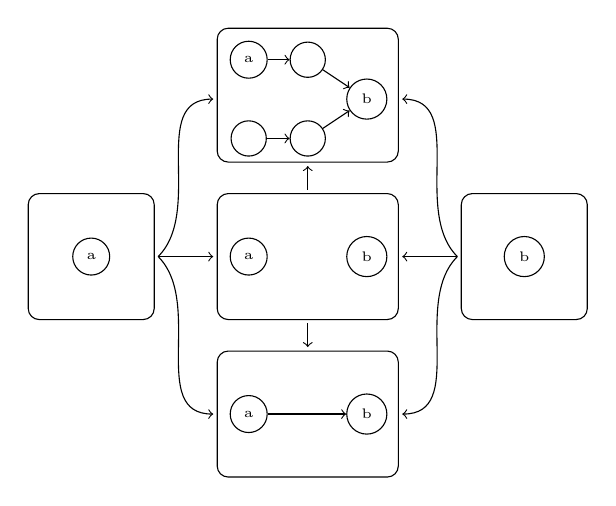
\begin{tikzpicture}[baseline=(current bounding box.center)]
	\draw[rounded corners] (1.6,-0.3) rectangle (3.9,1.3);
	\draw[rounded corners] (1.6,1.7) rectangle (3.9,3.3);
	\draw[rounded corners] (1.6,3.7) rectangle (3.9,5.4);
	\draw[rounded corners] (-0.8,1.7) rectangle (0.8,3.3);
	\draw[rounded corners] (4.7,1.7) rectangle (6.3,3.3);
	%
	\node[circle,draw] (ai) at (0,2.5) {\tiny a};
	\node[circle,draw] (bo) at (5.5,2.5) {\tiny b};
	\node[circle,draw] (a1) at (2,5) {\tiny a};
	\node[circle,draw,inner sep=4.5pt] (b1) at (2.75,5) {};
	\node[circle,draw,inner sep=4.5pt] (c1) at (2,4) {};
	\node[circle,draw,inner sep=4.5pt] (d1) at (2.75,4) {};
	\node[circle,draw] (e1) at (3.5,4.5) {\tiny b};
	\node[circle,draw] (a2) at (2,2.5) {\tiny a};
	\node[circle,draw] (b2) at (3.5,2.5) {\tiny b};
	\node[circle,draw] (a3) at (2,0.5) {\tiny a};
	\node[circle,draw] (b3) at (3.5,0.5) {\tiny b};
	%
	\draw [->] (a1) edge (b1);
	\draw [->] (b1) edge (e1);
	\draw [->] (c1) edge (d1);
	\draw [->] (d1) edge (e1);
	\draw [->] (a3) edge (b3);
	%
	\path [->] (0.85,2.5) edge[out=0,in=180] (1.55,2.5);
	\path [->] (0.85,2.5) edge[out=45,in=180] (1.55,4.5);
	\path [->] (0.85,2.5) edge[out=-45,in=180] (1.55,0.5);
	\path [->] (4.65,2.5) edge[out=180,in=0] (3.95,2.5);
	\path [->] (4.65,2.5) edge[out=135,in=0] (3.95,4.5);
	\path [->] (4.65,2.5) edge[out=225,in=0] (3.95,0.5);
	\draw [->] (2.75,3.35) -- (2.75,3.65);
	\draw [->] (2.75,1.65) -- (2.75,1.35);
\end{tikzpicture}
\end{equation}
However, $\cat{Rewrite}$ is not of interest in itself, but rather as an ambient context in which to generate a compact closed symmetric monoidal bicategory from some collection of morphisms and $2$-morphisms. Of course, which collection depends on one's interest.  We will illustrate this by considering the bicategory generated by a commutative Frobenius monoid. The diagram in \eqref{diag:MonoidUnit} serves as the unit law.  
 
The structure of the paper is as follows.  In Section \ref{sec:Span cospan bicats}, we introduce the three types of bicategories that we will be studying.  Then in Section \ref{sec:DoubleCategories}, we show how double categories can be used to show that bicategories have symmetric monoidal structure and also discuss various notions of duality in bicategories.  Nothing in that section is new, but we will use those results in Sections \ref{sec:SpansMaps}, \ref{sec:SpansSpans}, and \ref{sec:SpansCospans} to show that the bicategories of interest are symmetric monoidal and compact closed, and also fully dualizable in the case of the bicategories of spans of spans.  Finally, in Section \ref{sec:Applications}, we discuss two applications for bicategories of spans and cospans.  The first application is constructing a bicategory of spans of spans of groupoids that we conjecture is biequivalent to the bicategory conjectured by Morton and Vicary \cite{MortVic}.  The second is applying the bicategory of monic spans of cospans of directed graphs to rewriting graphs.


%%%%%%%%%%%%%%%%%%%%%%%%%%%%%%%%%%%%%%%%%%%%%%%%%%%%%%%%%%
%%%%%%%%%%%%%%%%%%%%%%%%%%%%%%%%%%%%%%%%%%%%%%%%%%%%%%%%%%
\section{Span and cospan bicategories} % EXAMPLES
\label{sec:Span cospan bicats}
%%%%%%%%%%%%%%%%%%%%%%%%%%%%%%%%%%%%%%%%%%%%%%%%%%%%%%%%%%
%%%%%%%%%%%%%%%%%%%%%%%%%%%%%%%%%%%%%%%%%%%%%%%%%%%%%%%%%%

Here we introduce three types of span and cospan bicategories.  Nothing in this section is new, but it provides a quick refresher as well as allows us to set our notation.  Throughout this paper, $\cat{C}$ will be a category with finite limits with chosen binary products and pullbacks and $\cat{D}$ will be a category with finite colimits with chosen binary coproducts and pushouts.  

One of the first examples given of a bicategory \cite{Be} is $\bispmap{C}$ whose objects are the $\cat{C}$-objects, morphisms $x \to z$ are given by $\cat{C}$-spans 
\[
	x \gets y \to z 
\]
which we denote by $y \from x \tospan z$ when convenient, and $2$-morphisms 
\[
	(y \from x \tospan z) \Rightarrow (y \from x' \tospan z)
\] 
are given by maps of spans
\[
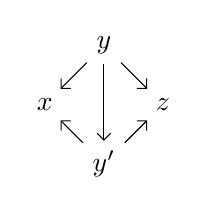
\begin{tikzpicture}
	\node (A) at (0,0) {$x$};
	\node (B) at (0.75,0.75) {$y$};
	\node (B') at (0.75,-0.75) {$y'$};
	\node (C) at (1.5,0) {$z$};
	%
	\path[->,font=\scriptsize,>=angle 90]
	(B) edge node[above]{$ $} (A)
	(B') edge node[above]{$ $} (A)
	(B) edge node[above]{$ $} (C)
	(B') edge node[above]{$ $} (C)
	(B) edge node[left]{$ $} (B');
\end{tikzpicture}
\]
There is a similar category denoted $\bicspmap{D}$ consisting of $\cat{D}$-objects, $\cat{D}$-cospans which we denote $y \from x \tocospan z$, and maps of $\cat{D}$-cospans given by diagrams  
\[
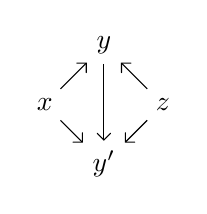
\begin{tikzpicture}
	\node (A) at (0,0) {$x$};
	\node (B) at (0.75,0.75) {$y$};
	\node (B') at (0.75,-0.75) {$y'$};
	\node (C) at (1.5,0) {$z$};
	%
	\path[->,font=\scriptsize,>=angle 90]
	(A) edge node[above]{$ $} (B)
	(A) edge node[above]{$ $} (B')
	(C) edge node[above]{$ $} (B)
	(C) edge node[above]{$ $} (B')
	(B) edge node[left]{$ $} (B');
\end{tikzpicture}
\]

Another way of promoting (co)span categories to bicategories is to consider different $2$-morphisms.  For example, Rebro \cite{Reb} constructed a bicategory $\bispsp{C}$ with $\cat{C}$-objects, $\cat{C}$-spans, and isomorphism classes of $\cat{C}$-spans of spans, which are diagrams of the form
\[
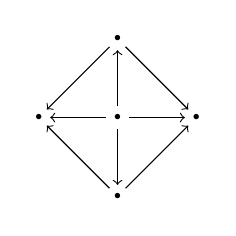
\begin{tikzpicture}[]
	\node[CDnode] (A) at (0,0) {$\bullet$};
	\node[CDnode] (B) at (1,1) {$\bullet$};
	\node[CDnode] (B') at (1,0) {$\bullet$};
	\node[CDnode] (B'') at (1,-1) {$\bullet$};
	\node[CDnode] (C) at (2,0) {$\bullet$};
	%
	\path[->,font=\scriptsize]
	(B) edge node[above]{$$} (A)
	(B) edge node[above]{$$} (C)
	(B') edge[->] node[left]{$$} (A)
	(B') edge[->] node[right]{$$} (C)
	(B'') edge node[left]{$$} (A)
	(B'') edge node[left]{$$} (C)
	(B') edge node[left]{$$} (B)
	(B') edge node[right]{$$} (B'');
\end{tikzpicture}
\]
Actually, the above diagram is an equivalence class of $2$-morphisms where we say two $2$-morphisms are equal if there is a $\cat{C}$-isomorphism $\theta$ such that the following diagram commutes.
\[
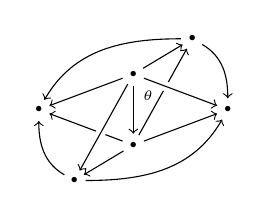
\begin{tikzpicture}[scale=0.6]
	\node[CDnode] (X) at (-2,0) {$\bullet$};
	\node[CDnode] (L) at (1.25,1.5) {$\bullet$};
	\node[CDnode] (Y) at (2,0) {$\bullet$};
	\node[CDnode] (S) at (-1.25,-1.5) {$\bullet$};
	\node[CDnode] (S'1) at (0,0.75) {$\bullet$};
	\node[CDnode] (S'2) at (0,-0.75) {$\bullet$};
	%
	\draw [<-] (X) edge[in=180,out=60] (L);
	\draw [<-] (X) edge[] (S'1);
	\draw [<-] (X) edge[] (S'2);
	\draw [<-] (X) edge[out=-90,in=150] (S);
	\draw [<-] (Y) edge[out=90,in=-30] (L);
	\draw [<-] (Y) edge[] (S'2);
	\draw [<-] (Y) edge[out=-120,in=0] (S);
	\draw [->] (S'1) edge[] (L);
	\draw [->] (S'1) edge[white,line width=3.5pt] (S);
	\draw [->] (S'1) edge[] (S);
	\draw [->] (S'1) edge node[right,pos=0.2,font=\tiny]{$\theta$} (S'2);
	\draw [->] (S'2) edge[] (L);
	\draw [->] (S'2) edge[] (S);
	\draw [<-] (Y) edge[white,line width=3.5pt] (S'1);
	\draw [<-] (Y) edge[] (S'1);
\end{tikzpicture}
\]
We will explore $\bispsp{C}$ more in Section \ref{subsec:SpanSpanGroupoid} where $\cat{D}$ is the category of groupoids and fibrations. Similarly, there is a dual bicategory $\bicspcsp{D}$ with $\cat{D}$-objects, $\cat{D}$-cospans, and isomorphism classes of $\cat{D}$-cospans of cospans

When studying `intercategories', Grandis and Par\'{e} \cite{GranPare_Intercats} looked at spans of cospans and found a lax interchange law. It was eventually shown that, under certain conditions, the interchange law is invertible \cite{Cic}. That is, while restricting attention to a topos $\cat{T}$, there is a bicategory $\bimonspcsp{T}$ with $\cat{T}$-objects, $\cat{T}$-cospans, and isomorphism classes of monic $\cat{T}$-spans of cospans. These $2$-morphisms are depicted as
\[
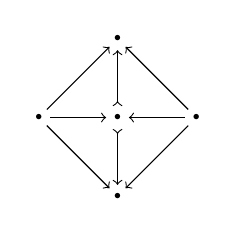
\begin{tikzpicture}[]
	\node[CDnode] (A) at (0,0) {$\bullet$};
	\node[CDnode] (B) at (1,1) {$\bullet$};
	\node[CDnode] (B') at (1,0) {$\bullet$};
	\node[CDnode] (B'') at (1,-1) {$\bullet$};
	\node[CDnode] (C) at (2,0) {$\bullet$};
	%
	\path[->,font=\scriptsize]
	(A) edge node[above]{$ $} (B)
	(A) edge node[above]{$ $} (B')
	(A) edge node[above]{$ $} (B'')
	(C) edge node[above]{$ $} (B)
	(C) edge node[above]{$ $} (B')
	(C) edge node[left]{$ $} (B'')
	(B') edge[>->] node[right]{$ $} (B)
	(B') edge[>->] node[left]{$ $} (B'');
\end{tikzpicture}
\]
This will be explored more is Section \ref{subsec:Rewrite} where we take $\cat{T}$ to be the topos of directed graphs. There is a dual bicategory $\biepiccspsp{T}$ with $\cat{T}$-objects, $\cat{T}$-spans, and isomorphism classes of epic $\cat{T}$-cospans of spans. 

%%%%%%%%%%%%%%%%
%%%%%%%%%%%%%%%%
\section{Double categories and duality} % DOUBLE CATS AND DUALITY SECTION
\label{sec:DoubleCategories}
%%%%%%%%%%%%%%%%
%%%%%%%%%%%%%%%%

Nothing in this section is new, but we will use the results presented here to show that the span and cospan bicategories from the previous section have symmetric monoidal and duality structures. The first subsection on double categories closely follows \cite{Shul}.  The second section discusses duality in bicategories. The material contained there can be found in \cite{Lurie,Piotr,Stay}.

%%%%%%%%%%%%%%%%%%%%%%%%%%%%%%%%%%%%%%%%%%%%%%%%%%%%%%%%%%
\subsection{Monoidal bicategories via double categories}
\label{subsec:DoubleCategories}
%%%%%%%%%%%%%%%%%%%%%%%%%%%%%%%%%%%%%%%%%%%%%%%%%%%%%%%%%%

Proving that the span and cospan bicategories are monoidal can be extremely tedious given the sheer number of axioms to check.  However, there is an easier method to show that a bicategory is symmetric monoidal due to Shulman \cite{Shul} which is to use double categories instead. Double categories, or pseudo double categories to be precise, have been studied by Fiore \cite{Fiore} and Par\'{e} and Grandis \cite{Gran}. Before formally defining them, it is helpful to have the following picture in mind. A double category has $2$-morphisms which look like

\begin{equation}
\label{diag:DblCatSquare}
\raisebox{-0.5\height}{
	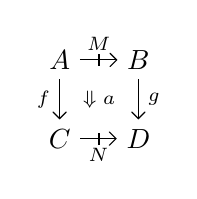
\begin{tikzpicture}
	\node (A) at (0,1) {$A$};
	\node (B) at (1,1) {$B$};
	\node (C) at (0,0) {$C$};
	\node (D) at (1,0) {$D$};
	%
	\path[->,font=\scriptsize,>=angle 90]
	(A) edge node[above]{$M$} (B)
	(A) edge node[left]{$f$} (C)
	(B) edge node[right]{$g$} (D)
	(C) edge node[below]{$N$} (D);
	%
	\draw (0.5,.925) -- (0.5,1.075);
	\draw (0.5,-.075) -- (0.5,.075);
	\node () at (0.5,0.5) {\scriptsize{$\Downarrow a$}};
	\end{tikzpicture}
}
\end{equation}
We call $A, B, C$ and $D$ \textbf{objects} or \textbf{0-cells}, $f$ and $g$ \textbf{vertical 1-morphisms}, $M$ and $N$ \textbf{horizontal 1-cells}, and $a$ a \textbf{2-morphism}. Note that a vertical 1-morphism is a morphism between 0-cells and a $2$-morphism is a morphism between horizontal 1-cells. We follow the notation of Shulman \cite{Shul} with the following definitions, using font as in `$\dblcat{D}$' as a stand-alone letter or as the first letter in a label or name to denote a `double category'.

% definition -- double category
%
\begin{defn}
	\label{def:DoubleCategory}
	A \textbf{pseudo double category} $\dblcat{D}$, or simply \textbf{double category}, consists of a category of objects $\dblcat{D}_{0}$ and a category of arrows $\dblcat{D}_{1}$ with the following functors
	\begin{equation*}
	\begin{split}
	U & \from \dblcat{D}_{0} \to \dblcat{D}_{1}, \\
	S,T & \from \dblcat{D}_{1} \rightrightarrows \dblcat{D}_{0}, \t{ and} \\
	\odot & \from \dblcat{D}_{1} \times_{\dblcat{D}_{0}} \dblcat{D}_{1} \to \dblcat{D}_{1}
	\end{split}
	\end{equation*}
	where the pullback $\dblcat{D}_{1} \times_{\dblcat{D}_{0}} \dblcat{D}_{1}$ is taken over $S$ and $T$.  These functors satisfy the equations
	\begin{equation*}
	\begin{split}
	S(U_{A}) = A &= T(U_{A}) \\
	S(M \odot N) & = SN \\
	T(M \odot N) & = TM. 
	\end{split}
	\end{equation*}
	This also comes equipped with natural isomorphisms
	\begin{equation*}
	\begin{split}
	\alpha & \from (M \odot N) \odot P \to M \odot (N \odot P)\\
	\lambda & \from U_{B} \odot M \to M\\
	\rho & \from M \odot U_{A} \to M
	\end{split}
	\end{equation*}
	such that $S(\alpha)$, $S(\lambda)$, $S(\rho)$, $T(\alpha)$, $T(\lambda)$, and $T(\rho)$ are all identities and that the coherence axioms of a monoidal category are satisfied. 
	
	To match this definition with the more intuitive terms used, we say \textbf{vertical 1-morphisms} for the $\dblcat{D}_{0}$-morphisms, \textbf{horizontal 1-cells} for the $\dblcat{D}_{1}$-objects, and \textbf{2-morphisms} for the $\dblcat{D}_{1}$-morphisms. As for notation, vertical and horizontal morphisms are written with the arrows $\to$ and $\hto$, respectively, and $2$-morphisms are drawn as in \eqref{diag:DblCatSquare}.
\end{defn}

An equivalent perspective to this definition is that a double category is simply a category that is `weakly internal' to $\cat{Cat}$. 

To bypass checking that a bicategory is monoidal, we will instead need to check that a double category is monoidal. To define a monoidal double category, however, we need the notion of a \textbf{globular 2-morphism}.  This is $2$-morphism whose source and target vertical morphisms are identities.

% Definition -- Monoidal Double Category
%
\begin{defn}
	\label{def:MonoidalDoubleCategory}
	A \textbf{monoidal double category} is a double category $\dblcat{D}$ equipped the following
	structure.
	\begin{enumerate}
		\item $\dblcat{D}_{0}$ and $\dblcat{D}_{1}$ are both monoidal categories.
		%
		\item If $I$ is the monoidal unit of $\dblcat{D}_{0}$, then $U_I$ is the
		monoidal unit of $\dblcat{D}_{1}$.
		%
		\item The functors $S$ and $T$ are strict monoidal, that is $S(M \otimes N)
		= SM \otimes SN$ and $T(M \otimes N)=TM \otimes TN$ and $S$ and $T$ also
		preserve the associativity and unit constraints.
		%
		\item We have globular $2$-isomorphisms
		\[ 
		\mathfrak{x} \from 
		(M_1 \otimes N_1) \odot (M_2 \otimes N_2) 
		\to 
		(M_1\odot M_2) \otimes (N_1\odot N_2)
		\]
		and
		\[
		\mathfrak{u} \from U_{A \otimes B} \to (U_A \otimes U_B)
		\]
		expressing that $\odot$ and $U$ are monoidal. Moreover, the following diagrams commute, expressing the constraint data for the double functor $\otimes$:
\item
		\[
		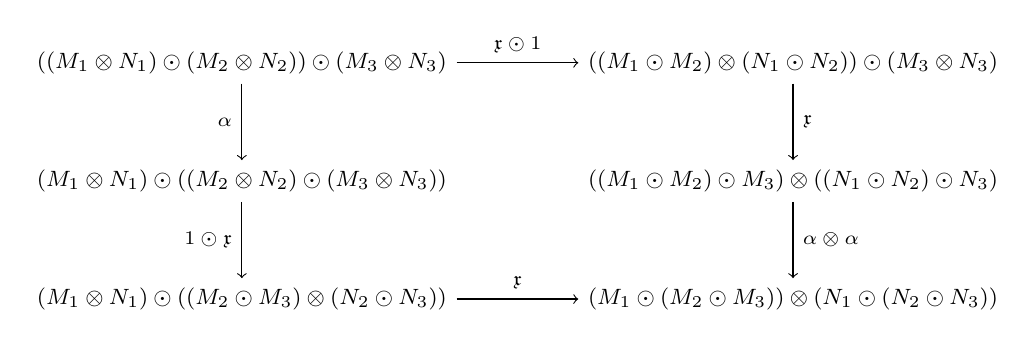
\begin{tikzpicture}
		\node (A) at (0,3) {\footnotesize{$((M_1\otimes N_1)\odot (M_2\otimes N_2)) \odot (M_3\otimes N_3)$}};
		\node (B) at (7,3) {\footnotesize{$((M_1\odot M_2)\otimes (N_1\odot N_2)) \odot (M_3\otimes N_3) $}};
		\node (A') at (0,1.5) {\footnotesize{$(M_1\otimes N_1)\odot ((M_2\otimes N_2) \odot (M_3\otimes N_3)) $}};
		\node (B') at (7,1.5) {\footnotesize{$((M_1\odot M_2)\odot M_3) \otimes ((N_1\odot N_2)\odot N_3)$}};
		\node (A'') at (0,0) {\footnotesize{$(M_1\otimes N_1) \odot ((M_2\odot M_3) \otimes (N_2\odot N_3))$}};
		\node (B'') at (7,0) {\footnotesize{$(M_1\odot (M_2\odot M_3)) \otimes (N_1\odot (N_2\odot N_3))$}};
		%
		\path[->,font=\scriptsize]
		(A) edge node[left]{$\alpha$} (A')
		(A') edge node[left]{$1 \odot \mathfrak{x}$} (A'')
		(B) edge node[right]{$\mathfrak{x}$} (B')
		(B') edge node[right]{$\alpha \otimes \alpha$} (B'')
		(A) edge node[above]{$\mathfrak{x} \odot 1$} (B)
		(A'') edge node[above]{$\mathfrak{x}$} (B'');
		\end{tikzpicture}
		\]
		\[
		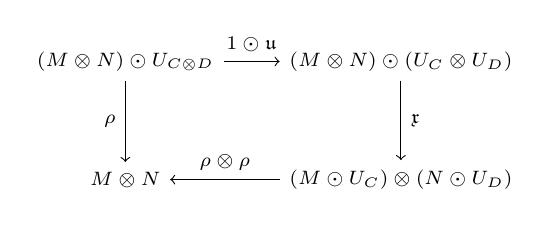
\begin{tikzpicture}
		\node (UL) at (0,1.5) {\scriptsize{$(M\otimes N) \odot U_{C\otimes D}$}};
		\node (LL) at (0,0) {\scriptsize{$M\otimes N$}};
		\node (UR) at (3.5,1.5) {\scriptsize{$(M\otimes N)\odot (U_C\otimes U_D)$}};
		\node (LR) at (3.5,0) {\scriptsize{$(M\odot U_C) \otimes (N\odot U_D)$}};
		%
		\path[->,font=\scriptsize]
		(UL) edge node[above]{$1 \odot \mathfrak{u}$} (UR) 
		(UL) edge node[left]{$\rho$} (LL)
		(LR) edge node[above]{$\rho \otimes \rho$} (LL)
		(UR) edge node[right]{$\mathfrak{x}$} (LR);
		\end{tikzpicture}
		%
		\quad
		%
		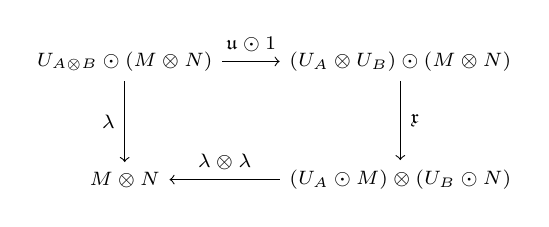
\begin{tikzpicture}
		\node (UL) at (0,1.5) {\scriptsize{$U_{A\otimes B}\odot (M\otimes N)$}};
		\node (LL) at (0,0) {\scriptsize{$M\otimes N$}};
		\node (UR) at (3.5,1.5) {\scriptsize{$(U_A\otimes U_B)\odot (M\otimes N)$}};
		\node (LR) at (3.5,0) {\scriptsize{$(U_A \odot M) \otimes (U_B\odot N)$}};
		%
		\path[->,font=\scriptsize]
		(UL) edge node[above]{$\mathfrak{u} \odot 1$} (UR) 
		(UL) edge node[left]{$\lambda$} (LL)
		(LR) edge node[above]{$\lambda \otimes \lambda$} (LL)
		(UR) edge node[right]{$\mathfrak{x}$} (LR);
		\end{tikzpicture}
		\]
		%
		\item The following diagrams commute, expressing that the
		associativity isomorphism for $\otimes$ is a transformation of double
		categories.
		\[
		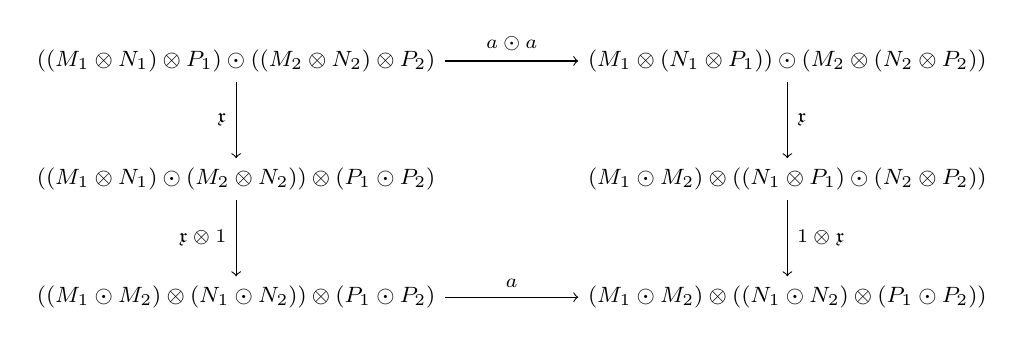
\begin{tikzpicture}
		\node (A) at (0,3) {\footnotesize{$((M_1\otimes N_1)\otimes P_1) \odot ((M_2\otimes N_2)\otimes P_2)$}};
		\node (B) at (7,3) {\footnotesize{$(M_1\otimes (N_1\otimes P_1)) \odot (M_2\otimes (N_2\otimes P_2))$}};
		\node (A') at (0,1.5) {\footnotesize{$((M_1\otimes N_1) \odot (M_2\otimes N_2)) \otimes (P_1\odot P_2)$}};
		\node (B') at (7,1.5) {\footnotesize{$(M_1\odot M_2) \otimes ((N_1\otimes P_1)\odot (N_2\otimes P_2))$}};
		\node (A'') at (0,0) {\footnotesize{$((M_1\odot M_2) \otimes(N_1\odot N_2)) \otimes (P_1\odot P_2)$}};
		\node (B'') at (7,0) {\footnotesize{$(M_1\odot M_2) \otimes ((N_1\odot N_2)\otimes (P_1\odot P_2))$}};
		%
		\path[->,font=\scriptsize]
		(A) edge node[left]{$\mathfrak{x}$} (A')
		(A') edge node[left]{$\mathfrak{x} \otimes 1$} (A'')
		(B) edge node[right]{$\mathfrak{x}$} (B')
		(B') edge node[right]{$1 \otimes \mathfrak{x}$} (B'')
		(A) edge node[above]{$a \odot a$} (B)
		(A'') edge node[above]{$a$} (B'');
		\end{tikzpicture}
		\]
		\[
		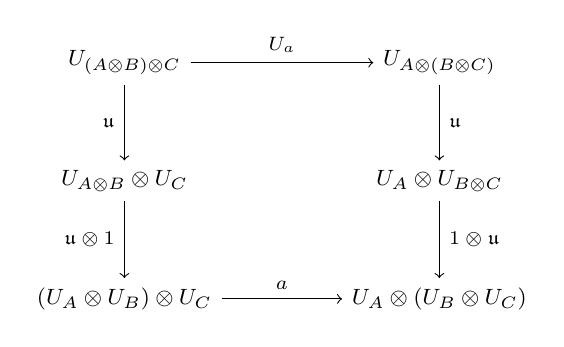
\begin{tikzpicture}
		\node (A) at (0,3) {\footnotesize{$U_{(A\otimes B)\otimes C}$}};
		\node (B) at (4,3) {\footnotesize{$U_{A\otimes (B\otimes C)} $}};
		\node (A') at (0,1.5) {\footnotesize{$U_{A\otimes B} \otimes U_C $}};
		\node (B') at (4,1.5) {\footnotesize{$U_A\otimes U_{B\otimes C}$}};
		\node (A'') at (0,0) {\footnotesize{$(U_A\otimes U_B)\otimes U_C$}};
		\node (B'') at (4,0) {\footnotesize{$U_A\otimes (U_B\otimes U_C) $}};
		%
		\path[->,font=\scriptsize]
		(A) edge node[left]{$\mathfrak{u}$} (A')
		(A') edge node[left]{$\mathfrak{u} \otimes 1$} (A'')
		(B) edge node[right]{$\mathfrak{u}$} (B')
		(B') edge node[right]{$1 \otimes \mathfrak{u}$} (B'')
		(A) edge node[above]{$U_{a}$} (B)
		(A'') edge node[above]{$a$} (B'');
		\end{tikzpicture}
		\]
		\item The following diagrams commute, expressing that the unit
		isomorphisms for $\otimes$ are transformations of double categories.
		\[
		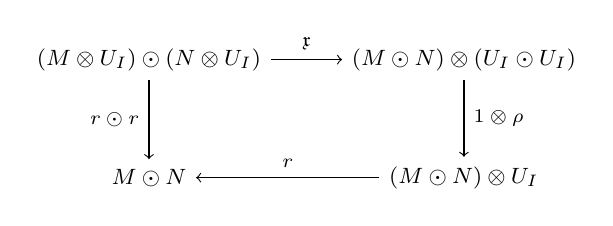
\begin{tikzpicture}
		\node (A) at (0,1.5) {\footnotesize{$(M\otimes U_I)\odot (N\otimes U_I)$}};
		\node (A') at (0,0) {\footnotesize{$M\odot N $}};
		\node (B) at (4,1.5) {\footnotesize{$(M\odot N)\otimes (U_I \odot U_I) $}};
		\node (B') at (4,0) {\footnotesize{$(M\odot N)\otimes U_I $}};
		%
		\path[->,font=\scriptsize]
		(A) edge node[left]{$r \odot r$} (A')
		(A) edge node[above]{$\mathfrak{x}$} (B)
		(B) edge node[right]{$1 \otimes \rho$} (B')
		(B') edge node[above]{$r$} (A');
		\end{tikzpicture}
		%
		\quad
		%
		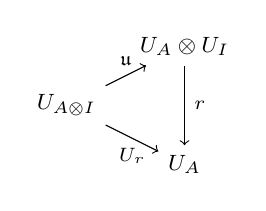
\begin{tikzpicture}
		\node (A) at (0,0.75) {\footnotesize{$U_{A\otimes I} $}};
		\node (B) at (1.5,1.5) {\footnotesize{$U_A\otimes U_I $}};
		\node (B') at (1.5,0) {\footnotesize{$U_A$}};
		%
		\path[->,font=\scriptsize]
		(A) edge node[above]{$\mathfrak{u}$} (B)
		(A) edge node[below]{$U_{r}$} (B')
		(B) edge node[right]{$r$} (B');
		\end{tikzpicture}
		\]
		%
		%
		%
		%
		\[
		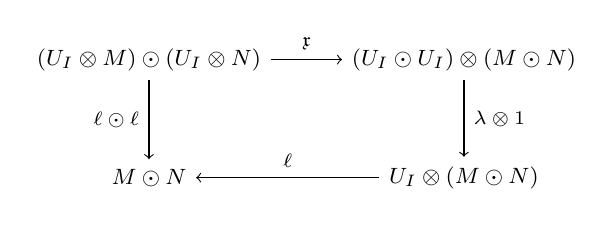
\begin{tikzpicture}
		\node (A) at (0,1.5) {\footnotesize{$(U_I\otimes M)\odot (U_I\otimes N)$}};
		\node (A') at (0,0) {\footnotesize{$M\odot N$}};
		\node (B) at (4,1.5) {\footnotesize{$(U_I \odot U_I) \otimes (M\odot N)$}};
		\node (B') at (4,0) {\footnotesize{$U_I\otimes (M\odot N) $}};
		%
		\path[->,font=\scriptsize]
		(A) edge node[left]{$\ell \odot \ell$} (A')
		(A) edge node[above]{$\mathfrak{x}$} (B)
		(B) edge node[right]{$\lambda \otimes 1$} (B')
		(B') edge node[above]{$\ell$} (A');
		\end{tikzpicture}
		%
		\quad
		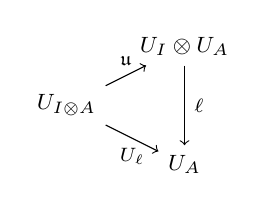
\begin{tikzpicture}
		\node (A) at (0,0.75) {\footnotesize{$U_{I\otimes A}$}};
		\node (B) at (1.5,1.5) {\footnotesize{$U_I\otimes U_A$}};
		\node (B') at (1.5,0) {\footnotesize{$U_A$}};
		%
		\path[->,font=\scriptsize]
		(A) edge node[above]{$\mathfrak{u}$} (B)
		(A) edge node[below]{$U_{\ell}$} (B')
		(B) edge node[right]{$\ell$} (B');
		\end{tikzpicture}
		\]
		\newcounter{mondbl}
		\setcounter{mondbl}{\value{enumi}}
	\end{enumerate}
	Similarly, a braided monoidal double category is a monoidal double
	category with the following additional structure.
	\begin{enumerate}
		\setcounter{enumi}{\value{mondbl}}
		\item $\dblcat{D}_{0}$ and $\dblcat{D}_{1}$ are braided monoidal categories.
		%
		\item The functors $S$ and $T$ are strict braided monoidal.
		%
		\item The following diagrams commute, expressing that the braiding is
		a transformation of double categories.
		\[
		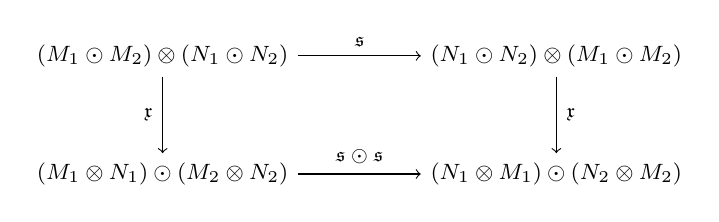
\begin{tikzpicture}
		\node (A) at (0,1.5) {\footnotesize{$(M_1 \odot M_2) \otimes (N_1 \odot N_2)$}};
		\node (A') at (0,0) {\footnotesize{$(M_1\otimes N_1) \odot (M_2\otimes N_2)$}};
		\node (B) at (5,1.5) {\footnotesize{$(N_1\odot N_2) \otimes (M_1 \odot M_2)$}};
		\node (B') at (5,0) {\footnotesize{$(N_1 \otimes M_1) \odot (N_2 \otimes M_2)$}};
		%
		\path[->,font=\scriptsize]
		(A) edge node[left]{$\mathfrak{x}$} (A')
		(A) edge node[above]{$\mathfrak{s}$} (B)
		(B) edge node[right]{$\mathfrak{x}$} (B')
		(A') edge node[above]{$\mathfrak{s} \odot \mathfrak{s}$} (B');
		\end{tikzpicture}
		%
		\quad
		%
		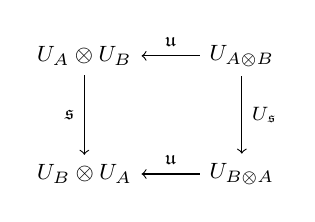
\begin{tikzpicture}
		\node (A) at (0,1.5) {\footnotesize{$U_A \otimes U_B$}};
		\node (A') at (0,0) {\footnotesize{$U_B\otimes U_A$}};
		\node (B) at (2,1.5) {\footnotesize{$U_{A\otimes B} $}};
		\node (B') at (2,0) {\footnotesize{$U_{B\otimes A}$}};
		%
		\path[->,font=\scriptsize]
		(A) edge node[left]{$\mathfrak{s}$} (A')
		(B) edge node[above]{$\mathfrak{u}$} (A)
		(B) edge node[right]{$U_\mathfrak{s}$} (B')
		(B') edge node[above]{$\mathfrak{u}$} (A');
		\end{tikzpicture}
		\]
		\setcounter{mondbl}{\value{enumi}}
	\end{enumerate}
	Finally, a symmetric monoidal double category is a monoidal double category $\mathbb{D}$ such that
	\begin{enumerate}
		\setcounter{enumi}{\value{mondbl}}
		\item $\dblcat{D}_{0}$ and $\dblcat{D}_{1}$ are in fact symmetric monoidal.
	\end{enumerate}
\end{defn}

%DEFINITION -- Companion and Conjoint
%
\begin{defn}
	\label{def:CompanionConjoint}
	Let $\mathbb{D}$ be a double category and $f \from A\to B$ a vertical morphism.  A \textbf{companion} of $f$ is a horizontal 1-cell
	$\widehat{f} \from A \hto B$ together with $2$-morphisms
	\[
	\raisebox{-0.5\height}{
		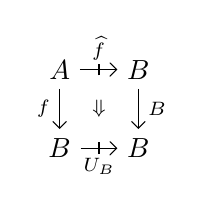
\begin{tikzpicture}
		\node (A) at (0,1) {$A$};
		\node (B) at (1,1) {$B$};
		\node (A') at (0,0) {$B$};
		\node (B') at (1,0) {$B$};
		%
		\path[->,font=\scriptsize,>=angle 90]
		(A) edge node[above]{$\widehat{f}$} (B)
		(A) edge node[left]{$f$} (A')
		(B) edge node[right]{$B$} (B')
		(A') edge node[below]{$U_B$} (B');
		%
		\draw (0.5,.925) -- (0.5,1.075);
		\draw (0.5,-.075) -- (0.5,.075);
		\node () at (0.5,0.5) {\scriptsize{$\Downarrow$}};
		\end{tikzpicture}
	}
	%
	\quad \text{and} \quad
	%
	\raisebox{-0.5\height}{
		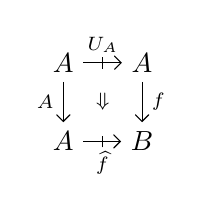
\begin{tikzpicture}
		\node (A) at (0,1) {$A$};
		\node (B) at (1,1) {$A$};
		\node (A') at (0,0) {$A$};
		\node (B') at (1,0) {$B$};
		%
		\path[->,font=\scriptsize,>=angle 90]
		(A) edge node[above]{$U_A$} (B)
		(A) edge node[left]{$A$} (A')
		(B) edge node[right]{$f$} (B')
		(A') edge node[below]{$\widehat{f}$} (B');
		%
		\draw (0.5,.925) -- (0.5,1.075);
		\draw (0.5,-.075) -- (0.5,.075);
		\node () at (0.5,0.5) {\scriptsize{$\Downarrow$}};
		\end{tikzpicture}
	}
	\]
	such that the following equations hold:
	\begin{equation}
	\label{eq:CompanionEq}
	\raisebox{-0.5\height}{
		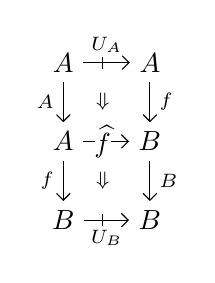
\begin{tikzpicture}
		\node (A) at (0,2) {$A$};
		\node (B) at (1.1,2) {$A$};
		\node (A') at (0,1) {$A$};
		\node (B') at (1.1,1) {$B$};
		\node (A'') at (0,0) {$B$};
		\node (B'') at (1.1,0) {$B$};
		%
		\path[->,font=\scriptsize,>=angle 90]
		(A) edge node[left]{$A$} (A')
		(A') edge node[left]{$f$} (A'')
		(B) edge node[right]{$f$} (B')
		(B') edge node[right]{$B$} (B'')
		(A) edge node[above]{$U_A$} (B)
		(A') edge  (B')
		(A'') edge node[below]{$U_B$} (B'');
		%
		\draw (0.5,1.925) -- (0.5,2.075);
		\draw[line width=2mm,white] (0.5,.925) -- (0.5,1.075);
		\draw (0.5,-.075) -- (0.5,.075);
		\node () at (0.5,0.5) {\scriptsize{$\Downarrow$}};
		\node () at (0.5,1.5) {\scriptsize{$\Downarrow$}};
		\node () at (0.5,1) {$\widehat{f}$};
		\end{tikzpicture}
	}
	%
	\raisebox{-0.5\height}{=}
	%
	\raisebox{-0.5\height}{
		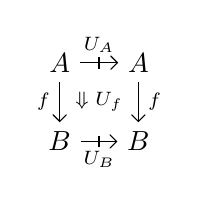
\begin{tikzpicture}
		\node (A) at (0,1) {$A$};
		\node (B) at (1,1) {$A$};
		\node (A') at (0,0) {$B$};
		\node (B') at (1,0) {$B$};
		%
		\path[->,font=\scriptsize,>=angle 90]
		(A) edge node[left]{$f$} (A')
		(B) edge node[right]{$f$} (B')
		(A) edge node[above]{$U_A$} (B)
		(A') edge node[below]{$U_B$} (B');
		%
		\draw (0.5,.925) -- (0.5,1.075);
		\draw (0.5,-.075) -- (0.5,.075);
		\node () at (0.5,0.5) {\scriptsize{$\Downarrow U_f$}};
		\end{tikzpicture}
	}
	%
	\raisebox{-0.5\height}{\text{   and   }}
	%
	\raisebox{-0.5\height}{
		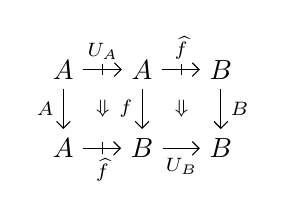
\begin{tikzpicture}
		\node (A) at (0,1) {$A$};
		\node (A') at (0,0) {$A$};
		\node (B) at (1,1) {$A$};
		\node (B') at (1,0) {$B$};
		\node (C) at (2,1) {$B$};
		\node (C') at (2,0) {$B$};
		%
		\path[->,font=\scriptsize,>=angle 90]
		(A) edge node[left]{$A$} (A')
		(B) edge node[left]{$f$} (B')
		(C) edge node[right]{$B$} (C')
		(A) edge node[above]{$U_A$} (B)
		(B) edge node[above]{$\widehat{f}$} (C)
		(A') edge node[below]{$\widehat{f}$} (B')
		(B') edge node[below]{$U_B$} (C');
		%
		\draw (1.5,0.925) -- (1.5,1.075);
		\draw (1.5,0.925) -- (1.5,1.075);
		\draw (0.5,.925) -- (0.5,1.075);
		\draw (0.5,-.075) -- (0.5,.075);
		\node () at (0.5,0.5) {\scriptsize{$\Downarrow$}};
		\node () at (1.5,0.5) {\scriptsize{$\Downarrow$}};
		\end{tikzpicture}
	}
	%
	\raisebox{-0.5\height}{=}
	%
	\raisebox{-0.5\height}{
		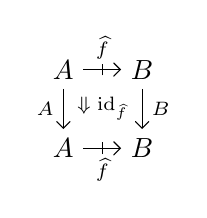
\begin{tikzpicture}
		\node (A) at (0,1) {$A$};
		\node (B) at (1,1) {$B$};
		\node (A') at (0,0) {$A$};
		\node (B') at (1,0) {$B$};
		%
		\path[->,font=\scriptsize,>=angle 90]
		(A) edge node[left]{$A$} (A')
		(B) edge node[right]{$B$} (B')
		(A) edge node[above]{$\widehat{f}$} (B)
		(A') edge node[below]{$\widehat{f}$} (B');
		%
		\draw (0.5,.925) -- (0.5,1.075);
		\draw (0.5,-.075) -- (0.5,.075);
		\node () at (0.5,0.5) {\scriptsize{$\Downarrow \id_{\widehat{f}}$}};
		\end{tikzpicture}
	}
	\end{equation}
	A \textbf{conjoint} of $f$, denoted $\check{f} \from B \hto A$, is a companion of $f$ in the double category $\dblcat{D}^{h\cdot\mathrm{op}}$ obtained by reversing the horizontal 1-cells, but not the vertical 1-morphisms, of $\dblcat{D}$.
\end{defn}

\begin{defn}
	\label{def:Fibrant}
	We say that a double category is \textbf{fibrant} if every vertical 1-morphism has both a companion and a conjoint. If every invertible vertical 1-morphism has both a companion and a conjoint, then we say the double category is \textbf{isofibrant}.
\end{defn}

Before we give the theorem that associates a symmetric monoidal bicategory to a suitable symmetric monoidal double category, we are first interested in how to get an ordinary bicategory from a double category. Indeed, for a double category $\dblcat{D}$, the \textbf{horizontal edge bicategory} $H(\dblcat{D})$ of $\dblcat{D}$ is the bicategory whose objects are those of $\dblcat{D}$, morphisms are horizontal 1-cells of $\dblcat{D}$, and $2$-morphisms are the globular $2$-morphisms.

\begin{thm}[Shulman {\cite[Theorem 5.1]{Shul}}]
	\label{thm:DoubleGivesBi}
	Let $\dblcat{D}$ be an isofibrant symmetric monoidal double category. Then $H(\dblcat{D})$ is a symmetric monoidal bicategory.  
\end{thm}

%%%%%%%%%%%%%%%
\subsection{Duality in bicategories}
\label{sec:CompactClosed}
%%%%%%%%%%%%%%%

In this section, we introduce various notions of duality that occur in bicategories so that we can define a notion of compact closed bicategories in the vein of Stay \cite{Stay}.  The stronger notion of fully dualizable is defined as well. Throughout, we suppress the notation for a monoidal operation and instead write $LR$ for the monoidal product of objects $L$ and $R$ and $fg$ for the monoidal product of morphisms $f$ and $g$.  This will reserve the symbol `$\otimes$' for the horizontal composition functor in the definition of a bicategory.

\begin{defn}
	\label{def:DualPairCat}
	A \textbf{dual pair} in a monoidal category is a tuple $(L,R,e,c)$ with objects $L$ and $R$, called the left and right duals, and morphisms
	\[
		e \from LR \to I 
		\quad \quad 
		c \from I \to RL,
	\]
	called evaluation and coevaluation such that 
	\[
	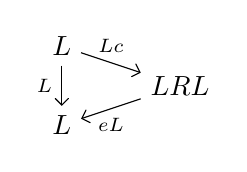
\begin{tikzpicture}
		\node (L1) at (0,1) {$L$};
		\node (L2) at (0,0) {$L$};
		\node (LRL) at (1.5,0.5) {$LRL$};
		%
		\path[->,font=\scriptsize,>=angle 90]
		(L1) edge node[left]{$L$} (L2)
		(L1) edge node[above]{$Lc$} (LRL)
		(LRL) edge node[below]{$eL$} (L2);
	\end{tikzpicture}
	%
	\quad \quad
	%
	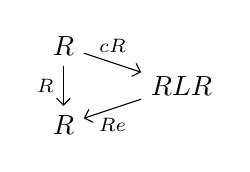
\begin{tikzpicture}
		\node (R1) at (0,1) {$R$};
		\node (R2) at (0,0) {$R$};
		\node (RLR) at (1.5,0.5) {$RLR$};
		%
		\path[->,font=\scriptsize,>=angle 90]
		(R1) edge node[left]{$R$} (R2)
		(R1) edge node[above]{$cR$} (RLR)
		(RLR) edge node[below]{$Re$} (R2);
	\end{tikzpicture}	
	\]
commute.
\end{defn}

\begin{defn}
	\label{def:DualPairBicat}
	A \textbf{dual pair} in a monoidal bicategory is a tuple $(L,R,e,c,\alpha,\beta)$ with objects $L$ and $R$, morphisms
	\[
		e \from LR \to I \quad \quad c \from I \to RL,
	\]
	and invertible $2$-morphisms
	\[
	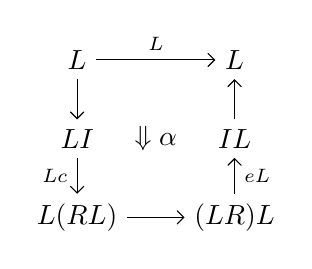
\begin{tikzpicture}
		\node (L1) at (0,2) {$L$};
		\node (LI) at (0,1) {$LI$};
		\node (LRL1) at (0,0) {$L(RL)$};
		\node (LRL2) at (2,0) {$(LR)L$};
		\node (IL) at (2,1) {$IL$};
		\node (L2) at (2,2) {$L$};
		%
		\path[->,font=\scriptsize,>=angle 90]
		(L1) edge (LI)
		(LI) edge node[left] {$Lc$} (LRL1)
		(LRL1) edge (LRL2)
		(LRL2) edge node[right] {$eL$} (IL)
		(IL) edge (L2)
		(L1) edge node[above] {$L$} (L2);
		%
		\node () at (1,1) {$\Downarrow \alpha$};
	\end{tikzpicture}
	%
	\quad \quad
	%
	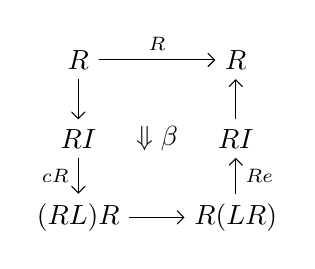
\begin{tikzpicture}
		\node (L1) at (0,2) {$R$};
		\node (LI) at (0,1) {$RI$};
		\node (LRL1) at (0,0) {$(RL)R$};
		\node (LRL2) at (2,0) {$R(LR)$};
		\node (IL) at (2,1) {$RI$};
		\node (L2) at (2,2) {$R$};
		%
		\path[->,font=\scriptsize,>=angle 90]
		(L1) edge (LI)
		(LI) edge node[left] {$cR$} (LRL1)
		(LRL1) edge (LRL2)
		(LRL2) edge node[right] {$Re$} (IL)
		(IL) edge (L2)
		(L1) edge node[above] {$R$} (L2);
		%
		\node () at (1,1) {$\Downarrow \beta$};
	\end{tikzpicture}
	\]
	called cusp isomorphisms.
	
	If this data satisfies the swallowtail equations in the sense that the diagrams in Figure \ref{fig:Swallowtail} are identities, then we call it a \textbf{coherent dual pair}.
\end{defn}

\begin{remark}
\label{rem:Swallowtail}
	To prevent cluttering the diagrams in Figure \ref{fig:Swallowtail}, we will only write $a,\rho,\lambda$ for the bicategory structure maps even when we actually mean their inverse, which should be clear from the context.
\end{remark}

\begin{figure}[h]
	%
	%  DIAGRAM 1
	%
	\[
	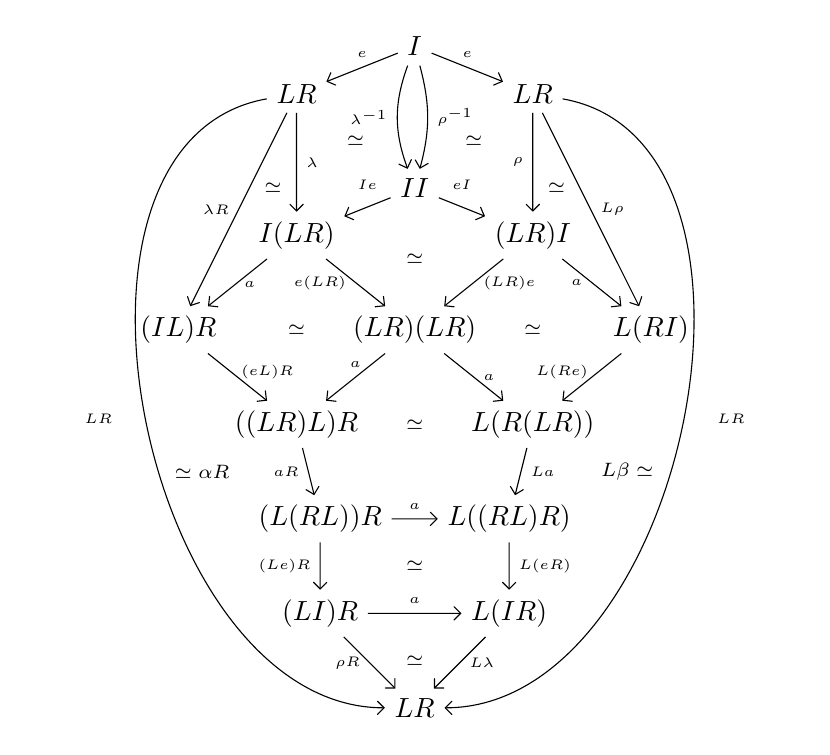
\begin{tikzpicture}[scale=0.60]
	\node (A) at (0,0) {$I$};
	\node (B) at (-2.5,-1) {$L R$};
	\node (C) at (2.5,-1) {$L R$};
	\node (D) at (0,-3) {$I I$};
	\node (E) at (-2.5,-4) {$I (L R)$};
	\node (F) at (2.5,-4) {$(L R) I$};
	\node (G) at (0,-6) {$(L R) (L R)$};
	\node (H) at (-5,-6) {$(I L) R$};
	\node (I) at (5,-6) {$L (R I)$};
	\node (J) at (-2.5,-8) {$((L R) L)  R$};
	\node (K) at (2.5,-8) {$L (R (L R))$};
	\node (L) at (-2,-10) {$(L (R L)) R$};
	\node (M) at (2,-10) {$L  ((R L) R)$};
	\node (N) at (-2,-12) {$(L I) R$};
	\node (O) at (2,-12) {$L (I R)$};
	\node (P) at (0,-14) {$L  R$};
	%
	%  2-CELLS
	%
	\node (Q) at (-1.25,-2) {\scriptsize{$\simeq$}};
	\node (R) at (1.25,-2) {\scriptsize{$\simeq$}};
	\node (S) at (0,-4.5) {\scriptsize{$\simeq$}};
	\node (T) at (-3,-3) {\scriptsize{$\simeq $}};
	\node (U) at (3,-3) {\scriptsize{$\simeq$}};
	\node (V) at (-2.5,-6) {\scriptsize{$\simeq$}};
	\node (W) at (2.5,-6) {\scriptsize{$\simeq$}};
	\node (X) at (0,-8) {\scriptsize{$\simeq$}};
	\node (Y) at (0,-11) {\scriptsize{$\simeq$}};
	\node (Z) at (0,-13) {\scriptsize{$\simeq$}};
	\node (A1) at (-4.5,-9) {\scriptsize{$\simeq \alpha R$}};
	\node (A2) at (4.5,-9) {\scriptsize{$L \beta \simeq$}};
	%
	\path[->,font=\tiny,>=angle 90]
	(A) edge node[above]{$e$} (B)
	(A) edge node[above]{$e$} (C)
	(A) edge[out=-110,in=110] node[left]{$\lambda^{-1}$} (D)
	(A) edge[out=-75,in=75] node[right]{$\rho^{-1}$} (D)
	(B) edge node[right]{$\lambda$}(E)
	(C) edge node[left]{$\rho$} (F)
	(D) edge node[left=0.2cm,above=0.1cm]{$I e$} (E)
	(D) edge node[left=0.2cm,above=0.1cm]{$e I$} (F)
	(E) edge node[below,left,pos=0.5]{$e (L R)$} (G)
	(F) edge node[below,right]{$(L R) e$} (G)
	(B) edge node[above,left]{$\lambda R$} (H)
	(C) edge node[above,right]{$L \rho$} (I)
	(E) edge node[below,right,pos=0.55]{$a$} (H)
	(F) edge node[below,left]{$a$} (I)
	(H) edge node[above,right,pos=0.4]{$(e L) R$} (J)
	(G) edge node[above]{$a$} (J)
	(I) edge node[above,left,pos=0.4]{$L (R e)$} (K)
	(G) edge node[above,right]{$a$} (K)
	(J) edge node[left]{$a R$} (L)
	(K) edge node[right]{$L a$} (M)
	(L) edge node[above]{$a$} (M)
	(L) edge node[left]{$(L  e) R$} (N)
	(M) edge node[right]{$L (e R)$} (O)
	(N) edge node[above]{$a$} (O)
	(N) edge node[below,left]{$\rho R$} (P)
	(O) edge node[below,right]{$L \lambda$} (P)
	(B) edge [out=-170,in=-180] node [below=0.3cm,left=0.3cm] {$L R$} (P)
	(C) edge [in=-360,out=-370,] node [below=0.3cm,right=0.3cm] {$LR$} (P);
	\end{tikzpicture}
	\]
	%
	%  DIAGRAM 2
	%
	\[
	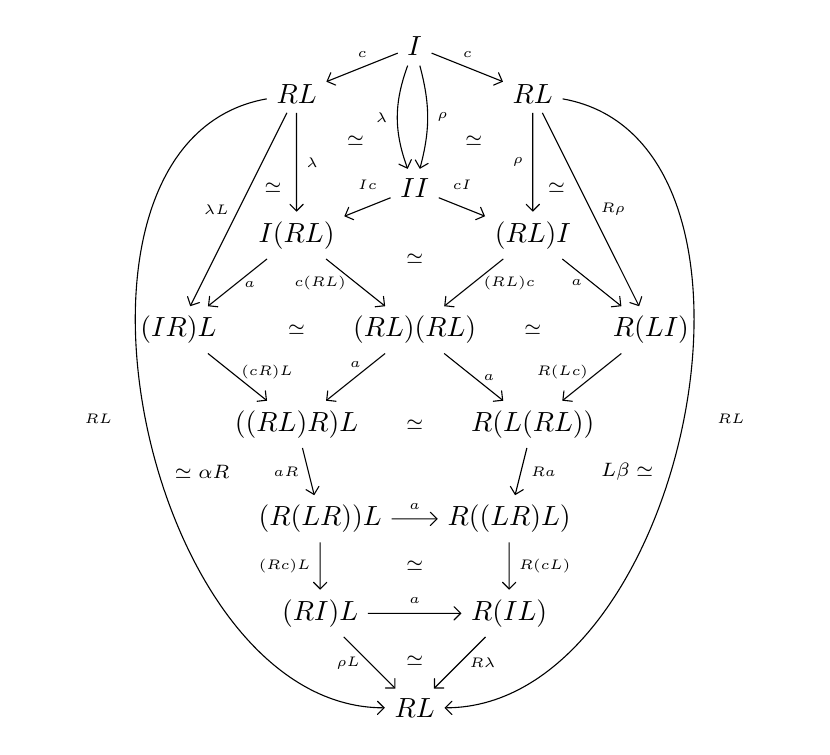
\begin{tikzpicture}[scale=0.60]
	\node (A) at (0,0) {$I$};
	\node (B) at (-2.5,-1) {$RL$};
	\node (C) at (2.5,-1) {$RL$};
	\node (D) at (0,-3) {$I I$};
	\node (E) at (-2.5,-4) {$I (RL)$};
	\node (F) at (2.5,-4) {$(RL) I$};
	\node (G) at (0,-6) {$(RL) (RL)$};
	\node (H) at (-5,-6) {$(I R) L$};
	\node (I) at (5,-6) {$R (L I)$};
	\node (J) at (-2.5,-8) {$((RL) R)  L$};
	\node (K) at (2.5,-8) {$R (L (R L))$};
	\node (L) at (-2,-10) {$(R (L R)) L$};
	\node (M) at (2,-10) {$R  ((L R) L)$};
	\node (N) at (-2,-12) {$(R I) L$};
	\node (O) at (2,-12) {$R (I L)$};
	\node (P) at (0,-14) {$R  L$};
	%
	%  2-CELLS
	%
	\node (Q) at (-1.25,-2) {\scriptsize{$\simeq$}};
	\node (R) at (1.25,-2) {\scriptsize{$\simeq$}};
	\node (S) at (0,-4.5) {\scriptsize{$\simeq$}};
	\node (T) at (-3,-3) {\scriptsize{$\simeq $}};
	\node (U) at (3,-3) {\scriptsize{$\simeq$}};
	\node (V) at (-2.5,-6) {\scriptsize{$\simeq$}};
	\node (W) at (2.5,-6) {\scriptsize{$\simeq$}};
	\node (X) at (0,-8) {\scriptsize{$\simeq$}};
	\node (Y) at (0,-11) {\scriptsize{$\simeq$}};
	\node (Z) at (0,-13) {\scriptsize{$\simeq$}};
	\node (A1) at (-4.5,-9) {\scriptsize{$\simeq \alpha R$}};
	\node (A2) at (4.5,-9) {\scriptsize{$L \beta \simeq$}};
	%
	\path[->,font=\tiny,>=angle 90]
	(A) edge[->] node[above]{$c$} (B)
	(A) edge[->] node[above]{$c$} (C)
	(A) edge[->,out=-110,in=110] node[left]{$\lambda$} (D)
	(A) edge[->,out=-75,in=75] node[right]{$\rho$} (D)
	(B) edge[->] node[right]{$\lambda$}(E)
	(C) edge[->] node[left]{$\rho$} (F)
	(D) edge[->] node[left=0.2cm,above=0.1cm]{$I c$} (E)
	(D) edge[->] node[left=0.2cm,above=0.1cm]{$c I$} (F)
	(E) edge[->] node[below,left,pos=0.5]{$c (R L)$} (G)
	(F) edge[->] node[below,right]{$(R L) c$} (G)
	(B) edge[->] node[above,left]{$\lambda L$} (H)
	(C) edge[->] node[above,right]{$R \rho$} (I)
	(E) edge[->] node[below,right,pos=0.55]{$a$} (H)
	(F) edge[->] node[below,left]{$a$} (I)
	(H) edge[->] node[above,right,pos=0.4]{$(c R) L$} (J)
	(G) edge[->] node[above]{$a$} (J)
	(I) edge[->] node[above,left,pos=0.4]{$R (L c)$} (K)
	(G) edge[->] node[above,right]{$a$} (K)
	(J) edge[->] node[left]{$a R$} (L)
	(K) edge[->] node[right]{$R a$} (M)
	(L) edge[->] node[above]{$a$} (M)
	(L) edge[->] node[left]{$(R  c) L$} (N)
	(M) edge[->] node[right]{$R (c L)$} (O)
	(N) edge[->] node[above]{$a$} (O)
	(N) edge[->] node[below,left]{$\rho L$} (P)
	(O) edge[->] node[below,right]{$R \lambda$} (P)
	(B) edge[->,out=-170,in=-180] node [below=0.3cm,left=0.3cm] {$R L$} (P)
	(C) edge[->,in=-360,out=-370] node [below=0.3cm,right=0.3cm] {$RL$} (P);
	\end{tikzpicture}
	\]
	\caption{The swallowtail diagrams for (co)evaluation}
	\label{fig:Swallowtail}
\end{figure}

Recall that a symmetric monoidal category is called \textbf{compact closed} if every object is part of a dual pair. We can generalize this idea to bicategories by introducing $2$-morphisms and some coherence axioms to ensure the $2$-morphisms play nicely. The following definition is due to Stay \cite{Stay}.

\begin{defn}
	\label{def:CompClosdBicat}
	A symmetric monoidal bicategory is called \textbf{compact closed} if each object $L$ has an associated coherent dual pair. 
\end{defn}

The difference between showing compact closededness in categories versus bicategories is quite large because of the swallowtail equations.  It is no surprise that these can be incredibly tedious to work with.  Fortunately, Pstragowski proved a wonderful strictification theorem that effectively circumvents the need to consider the swallowtail equations \cite[p.~22]{Piotr}.  

\begin{thm}[{\cite{Piotr}}]
	\label{thm:StrictingDualPairs}
	Given a dual pair $(L,R,e,c,\alpha,\beta)$, we can find a cusp isomorphism $\beta'$ such that $(L,R,e,c,\alpha,\beta')$ is a coherent dual pair.
\end{thm}

There is a striking resemblance between dual pairs as defined above and adjoint pairs. This similarity is worth exploring. Let's recall the unit-counit definition of a pair of adjoint functors.  Given a pair of functors $F \from \cat{A} \to \cat{B}$ and $G \from \cat{B} \to \cat{A}$, we say that they are an \textbf{adjoint pair} if there are natural isomorphisms $\eta \from \id_{A} \to GF$ and $\epsilon \from FG \to \id_B$ such that 
\[
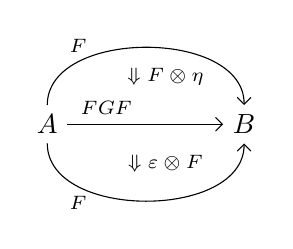
\begin{tikzpicture}
	\node (A) at (0,0) {$A$};
	\node (B) at (2.5,0) {$B$};
	%
	\path[->,font=\scriptsize,>=angle 90]
	(A) edge[out=90,in=90] node[above,pos=.25]{$F$} (B)
		edge node[above,pos=.25]{$FGF$} (B)
		edge[out=-90,in=-90] node[below,pos=.25]{$F$} (B);
	%
	\node () at (1.5,0.6) {\scriptsize{$\Downarrow F \otimes \eta$}};
	\node () at (1.5,-0.5) {\scriptsize{$\Downarrow \epsilon \otimes F$}};
\end{tikzpicture}
%
\quad \quad 
%
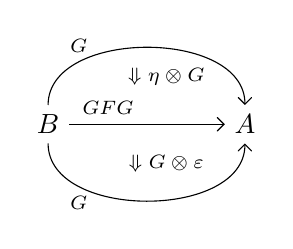
\begin{tikzpicture}
	\node (B) at (0,0) {$B$};
	\node (A) at (2.5,0) {$A$};
	%
	\path[->,font=\scriptsize,>=angle 90]
	(B) edge[out=90,in=90] node[above,pos=.25]{$G$} (A)
		edge node[above,pos=.25]{$GFG$} (A)
		edge[out=-90,in=-90] node[below,pos=.25]{$G$} (A);
	%
	\node () at (1.5,0.6) {\scriptsize{$\Downarrow \eta \otimes G$}};
	\node () at (1.5,-0.5) {\scriptsize{$\Downarrow G \otimes \epsilon$}};
\end{tikzpicture}
\]
each compose to their respective identity natural isomorphisms. Now, there is no reason for this sort of data to be restricted to only $\cat{Cat}$. Using the intuition from adjoint pairs in $\cat{Cat}$, we will generalize adjoints to arbitrary bicategories by replacing categories with objects, functors with morphisms, and natural transformations with $2$-morphisms.

\begin{defn}
	There is an \textbf{adjunction} between morphisms $f \from X \to Y$ and $g \from Y \to X$ in a bicategory if there are $2$-morphisms $\eta \from 1_{X} \to gf$ and $\epsilon \from fg \to 1_Y$ such that the compositions
	\[
	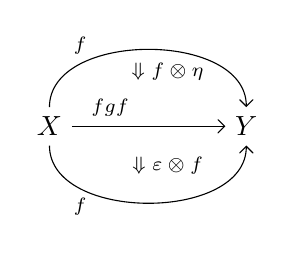
\begin{tikzpicture}
		\node (X) at (0,0) {$X$};
		\node (Y) at (2.5,0) {$Y$};
		%
		\path[->,font=\scriptsize,>=angle 90]
		(X) edge[out=90,in=90] node[above,pos=.25]{$f$} (Y)
			edge node[above,pos=.25]{$fgf$} (Y)
			edge[out=-90,in=-90] node[below,pos=.25]{$f$} (Y);
		%
		\node () at (1.5,0.7) {\scriptsize{$\Downarrow f \otimes \eta$}};
		\node () at (1.5,-0.5) {\scriptsize{$\Downarrow \epsilon \otimes  f$}};
	\end{tikzpicture}
	%
	\quad \quad 
	%
	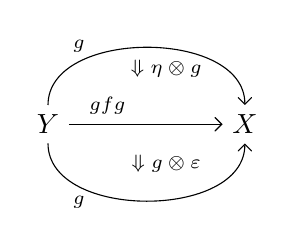
\begin{tikzpicture}
		\node (B) at (0,0) {$Y$};
		\node (A) at (2.5,0) {$X$};
		%
		\path[->,font=\scriptsize,>=angle 90]
		(B) edge[out=90,in=90] node[above,pos=.25]{$g$} (A)
			edge node[above,pos=.25]{$gfg$} (A)
			edge[out=-90,in=-90] node[below,pos=.25]{$g$} (A);
		%
		\node () at (1.5,0.7) {\scriptsize{$\Downarrow \eta \otimes g$}};
		\node () at (1.5,-0.5) {\scriptsize{$\Downarrow g \otimes \epsilon$}};
	\end{tikzpicture}
	\]
	each coincide with identity $2$-morphisms. Here, we say that $f$ is a left adjoint, $g$ is a right adjoint and write $f \dashv g$.  We also call $\eta$ the unit and $\epsilon$ the counit of the adjuntion. 
	
	An \textbf{equivalence} between objects $X$ and $Y$ in a bicategory consists of a pair of morphisms $f \from X \to Y$ and $g \from Y \to X$ and invertible $2$-morphisms $\eta \from fg \to \id_Y$ and $\epsilon \from \id_X \to gf$.  In the case that $\eta$ and $\epsilon$ are the unit of counit of an adjunction $f \dashv g$, we say there is an \textbf{adjoint equivalence}.
\end{defn}

The thing to do now is to recast the definitions of duality in terms of adjunctions.  The benefit of this is that it allows us to define a stronger condition than duals.

Recall that a monoidal category $\cat{M}$ can be thought of as a bicategory $\mathcal{B}\cat{M}$ with a single object, $\cat{M}$-objects as morphisms, and the $\cat{M}$-morphisms as the $2$-morphisms.  The composition functor of $\mathcal{B} \cat{M}$ is given by the monoidal structure of $\cat{M}$. Then, an $\cat{M}$-object $L$ has a right dual $R$ if and only if $L \dashv R$ in $\mathcal{B} \cat{M}$. 

Given a bicategory $\cat{B}$, define its homotopy category $\op{ho} \cat{B}$ by keeping the same objects and let the morphisms be isomorphism classes of morphisms. Now, suppose that $\cat{B}$ has a monoidal structure. The category $\op{ho} \cat{B}$ inherits this structure and so we can consider the bicategory $\mathcal{B} (\op{ho} \cat{B})$. This allows us to define duals in $\op{ho}\cat{B}$ via adjoints as above. A $\cat{B}$-object $L$ has a right dual if the $(\op{ho} \cat{B})$-object $L$ has a right dual.

Having seen dual pairs defined in terms of adjoints, we can go on to define an even stronger condition called `fully dual'.  We will take a simplified approach and only say enough for our needs. For a more fundamental and general account of full dualizability see \cite{Lurie,Piotr}. 

To prepare for the definition of fully dual pairs, we construct the following universal bicategory. Let $\cat{S}$ be a symmetric monoidal bicategory. There exists another symmetric monoidal bicategory $\cat{S}^{\text{fd}}$ with duals and a symmetric monoidal functor $i \from \cat{S}^{\text{fd}} \to \cat{S}$.  The idea behind the construction of $\cat{S}^{\text{fd}}$ is iterating a process of removing morphisms from $\cat{S}$ that do not have both a left or right adjoint. Then $\cat{S}^{\text{fd}}$ has the universal property where, given any other symmetric monoidal bicategory $\cat{S}'$ with duals and a symmetric monoidal functor $F \from \cat{S}' \to \cat{S}$, then $F$ factors uniquely up to isomorphism through $i$. Another way to think about $\cat{S}^{\text{fd}}$ is that it is the maximal sub-bicategory of $\cat{S}$ with respect to the property that every morphism has left and right adjoints.  

\begin{defn}
\label{def:FullDual}
	An object in a symmetric monoidal bicategory $\cat{S}$ is \textbf{fully dualizable} if it is in the essential image of $i \from \cat{S}^{\text{fd}} \to \cat{S}$
\end{defn}  

On the surface, it seems a bit dire to check whether an object is fully dualizable, but there is a nice characterization of this property that makes checking for it a bit easier.

\begin{thm}[Lurie {\cite[Prop.~4.2.3]{Lurie}}]
	An object in a bicategory is fully dualizable if it admits a dual and the evaluation map admits a left and right adjoint.  
\end{thm}

Suppose that we have an dual pair $(L,R,e,c,\alpha,\beta)$ in a bicategory and left adjoints $e^\text{L} \dashv e$ and $c^\text{L} \dashv c$.  There is a morphism $q$, called the \emph{Serre automorphism} of $L$, and its weak inverse $q^{-1}$ defined to be the respective composites
\begin{align*}
	L \to LI 
	\xto{Lc} LRL 
	\xto{\sigma L} RLL 
	\xto{c^\text{L}L} IL
	\to L \\
	L \to LI
	\xto{Le^\text{L}} LLR
	\xto{L\sigma} LRL
	\xto{eL} IL
	\to L.
\end{align*}
Lurie tells the story of why $q$ is named the Serre automorphism \cite[Remark 4.2.4]{Lurie}.  

\begin{defn}
	A fully dual pair $(L,R,e,c,\alpha,\beta)$ is \textbf{coherent} if it is coherent as a dual pair, there are left adjoints $e^{\text{L}}$ and $c^{\text{L}}$ so that the Serre automorphism pair $q,q^{-1}$ is an adjoint equivalence, and the composites diagrammed in Figures \ref{fig:CuspCounitsCompositeI} and \ref{fig:CuspCounitsCompositeII} are equal.  
\end{defn}

The coherence equation is a framed analogue of the cusp-flip relations in the presentation of the oriented bordism bicategory presented by Schommer-Pries in his thesis \cite{SchommerPries}.   They are further discussed by Schommer-Pries's student Pstrgowski in \cite{Piotr}.

\begin{figure}
\[
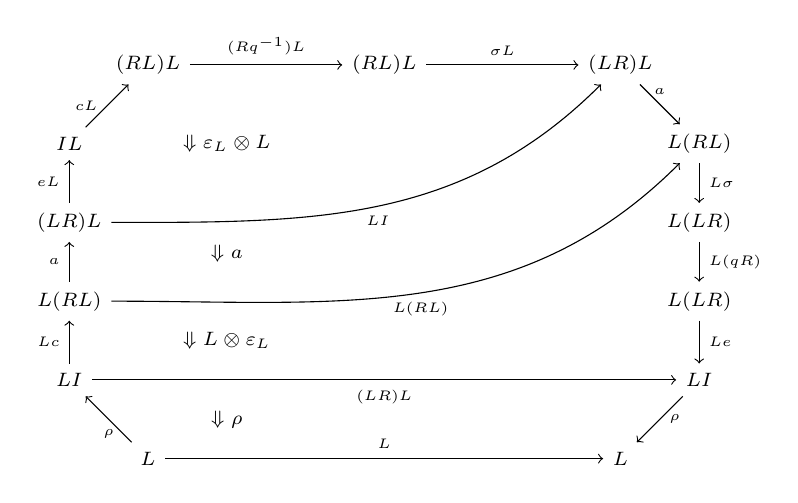
\begin{tikzpicture}
	%
	%  0-CELLS
	%
	\node (1) at (1,-2) {\scriptsize{$L$}};
	\node (2) at (0,-1) {\scriptsize{$LI$}};
	\node (3) at (0,0) {\scriptsize{$L(RL)$}};
	\node (4) at (0,1) {\scriptsize{$(LR)L$}};
	\node (5) at (0,2) {\scriptsize{$IL$}};
	\node (6) at (1,3) {\scriptsize{$(RL)L$}};
	\node (7) at (4,3) {\scriptsize{$(RL)L$}};
	\node (8) at (7,3) {\scriptsize{$(LR)L$}};
	\node (9) at (8,2) {\scriptsize{$L(RL)$}};
	\node (10) at (8,1) {\scriptsize{$L(LR)$}};
	\node (11) at (8,0) {\scriptsize{$L(LR)$}};
	\node (12) at (8,-1) {\scriptsize{$LI$}};
	\node (13) at (7,-2) {\scriptsize{$L$}};
	%
	%  1-CELLS
	%
	\path[->,font=\tiny]
	(1) edge node[left,below]{$\rho$} (2)
	(2) edge node[left]{$Lc$} (3)
	(3) edge node[left]{$a$} (4)
	(4) edge node[left]{$eL$} (5)
	(5) edge node[above,left]{$cL$} (6)
	(6) edge node[above]{$(Rq^{-1})L$} (7)
	(7) edge node[above]{$\sigma L$} (8)
	(8) edge node[above]{$a$} (9)
	(9) edge node[right]{$L \sigma$} (10)
	(10) edge node[right]{$L(qR)$} (11)
	(11) edge node[right]{$Le$} (12)
	(12) edge node[right]{$\rho$} (13)
	(1) edge node[above]{$L$} (13)
	%
	(2) edge node[below]{$(LR)L$} (12)
	(3) edge[out=0,in=225] node[below]{$L(RL)$} (9)
	(4) edge[out=0,in=225] node[below]{$LI$} (8);
	%
	%  2-CELLS
	%
	\node () at (2,2) {\scriptsize{$\Downarrow \epsilon_L \otimes L $}};
	\node () at (2,0.6) {\scriptsize{$\Downarrow a$}};
	\node () at (2,0-0.5) {\scriptsize{$\Downarrow L \otimes \epsilon_L$}};
	\node () at (2,-1.5) {\scriptsize{$\Downarrow \rho$}};
\end{tikzpicture}
\]
\caption{Cusp-Counits Composite I}
\label{fig:CuspCounitsCompositeI}
\end{figure}

\begin{figure}
\[
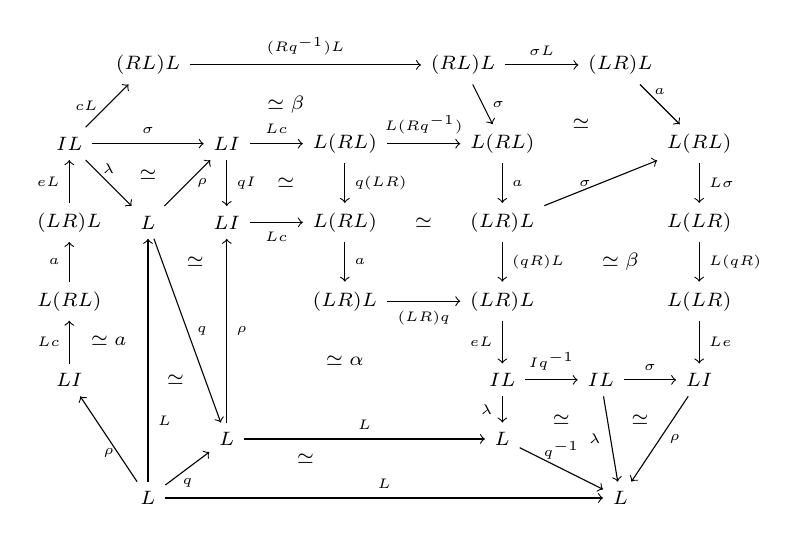
\begin{tikzpicture}
	%
	%  0-CELLS BOUNDARY
	%
	\node (1) at (1,-2.5) {\scriptsize{$L$}};
	\node (2) at (0,-1) {\scriptsize{$LI$}};
	\node (3) at (0,0) {\scriptsize{$L(RL)$}};
	\node (4) at (0,1) {\scriptsize{$(LR)L$}};
	\node (5) at (0,2) {\scriptsize{$IL$}};
	\node (6) at (1,3) {\scriptsize{$(RL)L$}};
	\node (7) at (5,3) {\scriptsize{$(RL)L$}};
	\node (8) at (7,3) {\scriptsize{$(LR)L$}};
	\node (9) at (8,2) {\scriptsize{$L(RL)$}};
	\node (10) at (8,1) {\scriptsize{$L(LR)$}};
	\node (11) at (8,0) {\scriptsize{$L(LR)$}};
	\node (12) at (8,-1) {\scriptsize{$LI$}};
	\node (13) at (7,-2.5) {\scriptsize{$L$}};
	%
	%  1-CELLS BOUNDARY
	%
	\path[->,font=\tiny]
	(1) edge node[left,below]{$\rho$} (2)
	(2) edge node[left]{$Lc$} (3)
	(3) edge node[left]{$a$} (4)
	(4) edge node[left]{$eL$} (5)
	(5) edge node[above,left]{$cL$} (6)
	(6) edge node[above]{$(Rq^{-1})L$} (7)
	(7) edge node[above]{$\sigma L$} (8)
	(8) edge node[above]{$a$} (9)
	(9) edge node[right]{$L \sigma$} (10)
	(10) edge node[right]{$L(qR)$} (11)
	(11) edge node[right]{$Le$} (12)
	(12) edge node[right]{$\rho$} (13)
	(1) edge node[above]{$L$} (13);
	%
	%  0-CELLS INTERIOR
	%
	\node (a) at (1,1) {\scriptsize{$L$}};
	\node (b) at (2,2) {\scriptsize{$LI$}};
	\node (b1) at (2,-1.75) {\scriptsize{$L$}};
	\node (c) at (2,1) {\scriptsize{$LI$}};
	\node (d) at (3.5,2) {\scriptsize{$L(RL)$}};
	\node (e) at (3.5,1) {\scriptsize{$L(RL)$}};
	\node (f) at (5.5,2) {\scriptsize{$L(RL)$}};
	\node (g) at (5.5,1) {\scriptsize{$(LR)L$}};
	\node (h) at (3.5,0) {\scriptsize{$(LR)L$}};
	\node (i) at (5.5,0) {\scriptsize{$(LR)L$}};
	\node (j) at (5.5,-1) {\scriptsize{$IL$}};
	\node (k) at (6.75,-1) {\scriptsize{$IL$}};
	\node (l) at (5.5,-1.75) {\scriptsize{$L$}};
	%
	%  1-CELLS INTERIOR
	%
	\path[->,font=\tiny]
	(5) edge node[above]{$\lambda$} (a)
	(1) edge node[right,pos=0.25]{$L$} (a)
	(a) edge node[below,right]{$\rho$} (b)
	(a) edge node[right]{$q$} (b1)
	(1) edge node[below]{$q$} (b1)
	(5) edge node[above]{$\sigma$} (b)
	(b) edge node[right]{$qI$} (c)
	(b1) edge node[right]{$\rho$} (c)
	(b) edge node[above]{$Lc$} (d)
	(c) edge node[below]{$Lc$} (e)
	(d) edge node[right]{$q(LR)$} (e)
	(d) edge node[above]{$L(Rq^{-1})$} (f)
	(7) edge node[right]{$\sigma$} (f)
	(f) edge node[right]{$a$} (g)
	(g) edge node[above,left]{$\sigma$} (9)
	(e) edge node[right]{$a$} (h)
	(g) edge node[right]{$(qR)L$} (i)
	(h) edge node[below]{$(LR)q$} (i)
	(i) edge node[left]{$eL$} (j)
	(j) edge node[above]{$Iq^{-1}$} (k)
	(k) edge node[above]{$\sigma$} (12)
	(k) edge node[left]{$\lambda$} (13)
	(b1) edge node[above]{$L$} (l)
	(j) edge node[left]{$\lambda$} (l)
	(l) edge node[above]{$q^{-1}$} (13);
	%
	%
	%  2-CELLS
	%
	\node () at (0.5,-0.5) {\scriptsize{$\simeq a$}};
	\node () at (1.35,-1) {\scriptsize{$\simeq$}};
	\node () at (1,1.6) {\scriptsize{$\simeq$}};
	\node () at (1.6,0.5) {\scriptsize{$\simeq$}};
	\node () at (2.75,1.5) {\scriptsize{$\simeq$}};
	\node () at (2.75,2.5) {\scriptsize{$\simeq \beta$}};
	\node () at (6.5,2.25) {\scriptsize{$\simeq$}};
	\node () at (4.5,1) {\scriptsize{$\simeq$}};
	\node () at (3.5,-0.75) {\scriptsize{$\simeq \alpha$}};
	\node () at (3,-2) {\scriptsize{$\simeq$}};
	\node () at (6.25,-1.5) {\scriptsize{$\simeq$}};
	\node () at (7.25,-1.5) {\scriptsize{$\simeq$}};
	\node () at (7,0.5) {\scriptsize{$\simeq \beta$}};
\end{tikzpicture}
\]
\caption{Cusp-Counits Composite II}
\label{fig:CuspCounitsCompositeII}
\end{figure}

\begin{thm}[{\cite[Thm.~3.16]{Piotr}}]
	Any fully dualizable object can be completed to a coherent fully dual pair.
\end{thm}
 

%%%%%%%%%%%%%%%%%%%%%%%%%%%%%%%%%%%%%%%%%%%%%%%%%%%%%%%%%%
%%%%%%%%%%%%%%%%%%%%%%%%%%%%%%%%%%%%%%%%%%%%%%%%%%%%%%%%%%
\section{(Co)spans and maps of (co)spans} % SPANS AND MAPS OF SPANS
\label{sec:SpansMaps}
%%%%%%%%%%%%%%%%%%%%%%%%%%%%%%%%%%%%%%%%%%%%%%%%%%%%%%%%%%
%%%%%%%%%%%%%%%%%%%%%%%%%%%%%%%%%%%%%%%%%%%%%%%%%%%%%%%%%%

In this section, we show that the bicategory $\bispmap{C}$ of $\cat{C}$-objects, $\cat{C}$-spans, and $\cat{C}$-maps of spans is symmetric monoidal. We also show that the the bicategory $\bicspmap{D}$ of $\cat{D}$-objects, $\cat{D}$-cospans, and $\cat{D}$-maps of cospans is a symmetric monoidal bicategory.  

To this end, we define double categories $\dblspmap{C}$ and $\dblcspmap{D}$.   The objects of $\dblspmap{C}$ are the $\cat{C}$-objects, vertical morphisms are the $\cat{C}$-morphisms, horizontal morphisms are $\cat{C}$-spans, and $2$-morphisms are triples of $\cat{C}$-morphisms between two spans in $\bold{C}$ so that the diagram
\[
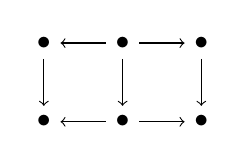
\begin{tikzpicture}
	\node (v1) at (-3.5,3.5) {$\bullet$};
	\node (v5) at (-1.5,3.5) {$\bullet$};
	\node (v3) at (-2.5,3.5) {$\bullet$};
	\node (v2) at (-3.5,2.5) {$\bullet$};
	\node (v6) at (-1.5,2.5) {$\bullet$};;
	\node (v4) at (-2.5,2.5) {$\bullet$};
	\draw [->]  (v1) edge (v2);
	\draw [->] (v3) edge (v4);
	\draw [->] (v5) edge (v6);
	\draw [->] (v3) edge (v5);
	\draw [->] (v3) edge (v1);
	\draw[->]  (v4) edge (v6);
	\draw [->] (v4) edge (v2);
\end{tikzpicture}
\]
commutes.  The dual double category $\dblcspmap{D}$ was introduced by Dawson, Par\'{e}, and Pronk \cite{DawsonParePronk} and discussed by one of the authors \cite{Cour}.

% SYMMETRIC MONOIDAL DOUBLE CATEGORIES
\begin{lem}[{\cite[Prop.~4.2]{Cour}}]
\label{lem:SpanMapsDoubleCat}
	The double categories $\dblspmap{C}$ and $\dblcspmap{D}$ are symmetric monoidal.  
\end{lem}

% ISOFIBRANT
\begin{lem}
	\label{lem:SpanMapsIsofibrant}
	The symmetric monoidal double categories $\dblspmap{C}$ and $\dblcspmap{D}$ are isofibrant.  
\end{lem}

\begin{proof}
	Let $f \from a \to b$ be a vertical morphism in $\dblcspmap{D}$.  The companion $\widehat{f}$ is the cospan 
	\[
		a \xto{f} b \gets b
	\]
	with the $2$-morphisms $\id_b$ and $f$.  The conjoint $\check{f}$ of $f$ is the cospan
	\[
	b \to b \xleftarrow{f} a
	\]
	equipped with the same two $2$-morphisms. 
\end{proof}

Using these Lemmas, we can use results from Shulman to obtain the main theorem of this section.

% SYMMETRIC MONOIDAL BICATEGORIES
\begin{thm}
\label{thm:SpansMapsAreSMBicat}
	The bicategories $\bispmap{C}$ and $\bicspmap{D}$ are symmetric monoidal.
\end{thm}

\begin{proof}
	Apply Theorem \ref{thm:DoubleGivesBi}.
\end{proof}

Having shown that the bicategories are symmetric monoidal, we now study their duality structures.

\begin{lem}
\label{lem:PushoutDiagram}
	The diagram
	\[
		\begin{tikzpicture}
			\node (UL) at (0,1) {$X+X+X$};
			\node (LL) at (0,0) {$X+X$};
			\node (UR) at (3,1) {$X+X$};
			\node (LR) at (3,0) {$X$};
			%
			\path[->,font=\scriptsize,>=angle 90]
			(UL) edge node[above] {$X+\nabla$} (UR)
			(UL) edge node[left] {$\nabla +X$} (LL)
			(UR) edge node[right] {$\nabla$} (LR)
			(LL) edge node[above] {$\nabla$} (LR);
		\end{tikzpicture}
	\]
	is a pushout square.
\end{lem}

\begin{proof}
	Suppose we have maps $f,g \from X+X \to Y$ that form a cocone over the span inside the above diagram. Let $\iota \from X \to X+X+X$ include $X$ into the middle copy of $X$. Observe that $\ell \coloneqq (\nabla + X) \circ \iota$ and $r \coloneqq (X + \nabla) \circ \iota$ are, respectively, the left and right inclusions $X \to X+X$. Then $f \circ \ell = g \circ r$ is a map $X \to Y$, which we claim is the unique map making the required diagram commute. Indeed, given $h \from X \to Y$ such that $f = h \circ \nabla = g$, then $g \circ r = f \circ \ell = h \circ \nabla \circ \ell = h$.
\end{proof}

\begin{thm}
	\label{thm:SpansMapsAreCCBicat}
	The bicategories $\bispmap{C}$ and $\bicspmap{D}$ are compact closed.
\end{thm}

\begin{proof}
	We will prove this for $\bicspmap{D}$ and use duality to obtain the result for $\bispmap{C}$. To begin, we will show that objects are self dual. Take an object $X$.  Define the evaluation morphism $e \from X + X \tocospan 0$ and coevaluation morphism $c \from 0 \tocospan X+X$ to be the following cospans:
	\[
		e = (X+X \xto{\nabla} X \gets 0), \quad \quad 
		c = (0 \to X \xleftarrow{\nabla} X+X).
	\]
	Next we define the cusp isomorphisms, $\alpha$ and $\beta$.
	Note that $\alpha$ is a $2$-morphism whose domain is the composite morphism
	\[
		X \xto{\ell}
		X+X \xleftarrow{X+\nabla}
		X+X+X \xto{\nabla +X}
		X+X \xleftarrow{r}
		X
	\]
	and whose codomain is the identity cospan on $X$.  Use Lemma \ref{lem:PushoutDiagram} and the fact that $\nabla+X = \ell \circ \nabla$ and $X + \nabla = r \circ \nabla$ to see that the composite is the identity cospan on $X$.  The codomain of $\beta$ is also the identity cospan on $X$, which is obtained as the composite morphism
	\[
		X \xto{r}
		X+X \xleftarrow{\nabla+X}
		X+X+X \xto{X+\nabla}
		X+X \xleftarrow{\ell}
		X
	\]
	Take $\alpha$ and $\beta$, each, to be the identity $2$-morphism on $X$. Thus we have a dual pair $(X,X,e,c,\alpha,\beta)$. By Theorem \ref{thm:StrictingDualPairs}, we know there is a cusp isomorphism $\beta'$ such that $(X,X,e,c,\alpha,\beta')$ is a coherent dual pair.  
\end{proof}

%%%%%%%%%%%%%%%%%%%%%%%%%%%%%%%%%%%%%%%%%%%%%%%%%%%%%%%%%%
%%%%%%%%%%%%%%%%%%%%%%%%%%%%%%%%%%%%%%%%%%%%%%%%%%%%%%%%%%
% SPANS AND SPANS OF SPANS + OP
\section{(Co)spans and (co)spans of (co)spans}                  
\label{sec:SpansSpans}
%%%%%%%%%%%%%%%%%%%%%%%%%%%%%%%%%%%%%%%%%%%%%%%%%%%%%%%%%%
%%%%%%%%%%%%%%%%%%%%%%%%%%%%%%%%%%%%%%%%%%%%%%%%%%%%%%%%%%

In this section, we will show that the bicategories $\bispsp{C}$ and $\bicspcsp{D}$ are symmetric monoidal. Again, we will only prove this for $\bicspcsp{D}$ and note that an analogous argument will show that the same holds for $\bispsp{C}$.  

\begin{defn}
\label{def:DblCatSpanSpan}
	Define a double category $\dblspsp{C}$ whose objects are the $\cat{C}$-objects, vertical morphisms are given by isomorphism classes of $\cat{C}$-spans, horizontal morphisms are given by $\cat{C}$-spans, and $2$-morphisms are spans of spans in $\cat{C}$ making the evident diagram commute (see Figure \ref{fig:2cells}). Define the double category $\dblcspcsp{D}$ by replacing $\cat{C}$ with $\cat{D}$ and spans with cospans.  
\end{defn}

% DOUBLE CATEGORIES
\begin{lem}
	\label{lem:SpanSpanDoubleCat}
	Both $\dblspsp{C}$ and $\dblcspcsp{D}$ are actually double categories.  
\end{lem}

\begin{proof}
	We will prove this for the case of $\dblcspcsp{D}$. To simplify notation, we will denote $\dblcspcsp{D}$ by $\dblcat{D}$.
	
	The object category $\dblcat{D}_0$ is the usual category $\cat{Csp(D)}$ of isomorphism classes of cospans in $\bold{D}$.  The arrow category $\dblcat{D}_1$ has as objects as $\cat{D}$-cospans and morphisms as isomorphism classes of cospans of cospans. A morphism from $b \from a \tocospan c$ to $b'' \from a'' \tocospan c''$ is given by a diagram
	\begin{equation}
	\label{diag:CspCsp2Cell}
	\raisebox{-0.5\height}{
	\begin{tikzpicture}
		\node (A) at (0,2) {$a$};
		\node (A') at (0,1) {$a'$};
		\node (A'') at (0,0) {$a''$};
		\node (B) at (1,2) {$b$};
		\node (B') at (1,1) {$b'$};
		\node (B'') at (1,0) {$b''$};
		\node (C) at (2,2) {$c$};
		\node (C') at (2,1) {$c'$};
		\node (C'') at (2,0) {$c''$};
		%
		\path[->,font=\scriptsize,>=angle 90]
		% horizontal arrows
		(A) edge node[above]{$$} (B)
		(A') edge node[above]{$$} (B')
		(A'') edge node[above]{$$} (B'')
		(C) edge node[above]{$$} (B)
		(C') edge node[above]{$$} (B')
		(C'') edge node[above]{$$} (B'')
		% vertical arrows
		(A) edge node[left]{$$} (A')
		(A'') edge node[left]{$$} (A')
		(B) edge node[left]{$$} (B')
		(B'') edge node[left]{$$} (B')
		(C) edge node[left]{$$} (C')
		(C'') edge node[left]{$$} (C');	
	\end{tikzpicture}
	}
	\end{equation}
	It is straightforward enough to check that $\dblcat{D}_1$ is a category.
	
	The unit functor $U \from \dblcat{D}_0 \to \dblcat{D}_1$ maps a $\dblcat{D}$-object to the identity cospan on it and a morphism, $b \from a \tocospan c$ to the square 
	\[
	\begin{tikzpicture}
		\node (A) at (0,2) {$a$};
		\node (A') at (0,1) {$a$};
		\node (A'') at (0,0) {$a$};
		\node (B) at (1,2) {$b$};
		\node (B') at (1,1) {$b$};
		\node (B'') at (1,0) {$b$};
		\node (C) at (2,2) {$c$};
		\node (C') at (2,1) {$c$};
		\node (C'') at (2,0) {$c$};
		%
		\path[->,font=\scriptsize,>=angle 90]
		% horizontal arrows
		(A) edge node[above]{$ $} (B)
		(A') edge node[above]{$ $} (B')
		(A'') edge node[above]{$ $} (B'')
		(C) edge node[above]{$ $} (B)
		(C') edge node[above]{$ $} (B')
		(C'') edge node[above]{$ $} (B'')
		% vertical arrows
		(A) edge node[left]{$a$} (A')
		(A'') edge node[left]{$a$} (A')
		(B) edge node[left]{$b$} (B')
		(B'') edge node[left]{$b$} (B')
		(C) edge node[left]{$c$} (C')
		(C'') edge node[left]{$c$} (C');	
	\end{tikzpicture}
	\]
	%
	The source functor $S \from \dblcat{D}_1 \to \dblcat{D}_0$ sends an object $b \from a \tocospan c$ to $a$ and a morphism, say \eqref{diag:CspCsp2Cell}, to $b \from a \tocospan c$.  
	%
	The target functor $T$ is defined similarly. These structure functors satisfy the required equations.  
	
	We can illustrate the action of the composition functor $ \odot \from \dblcat{D}_1 \times_{\dblcat{D}_0} \dblcat{D}_1 \to \dblcat{D}_1$ diagramatically as
	\[
	\raisebox{-0.5\height}{
	\begin{tikzpicture}
		\node (A) at (0,2) {$a$};
		\node (A') at (0,1) {$a'$};
		\node (A'') at (0,0) {$a''$};
		\node (B) at (1,2) {$b$};
		\node (B') at (1,1) {$b'$};
		\node (B'') at (1,0) {$b''$};
		\node (C) at (2,2) {$c$};
		\node (C') at (2,1) {$c'$};
		\node (C'') at (2,0) {$c''$};
		\node (D) at (3,2) {$d$};
		\node (D') at (3,1) {$d'$};
		\node (D'') at (3,0) {$d''$};
		\node (E) at (4,2) {$e$};
		\node (E') at (4,1) {$e'$};
		\node (E'') at (4,0) {$e''$};
		%
		\path[->,font=\scriptsize,>=angle 90]
		% horizontal arrows
		(A) edge node[above]{$$} (B)
		(A') edge node[above]{$$} (B')
		(A'') edge node[above]{$$} (B'')
		(C) edge node[above]{$$} (B)
		(C') edge node[above]{$$} (B')
		(C'') edge node[above]{$$} (B'')
		(C) edge node[above]{$$} (D)
		(C') edge node[above]{$$} (D')
		(C'') edge node[above]{$$} (D'')
		(E) edge node[above]{$$} (D)
		(E') edge node[above]{$$} (D')
		(E'') edge node[above]{$$} (D'')
		% vertical arrows
		(A) edge node[left]{$$} (A')
		(A'') edge node[left]{$$} (A')
		(B) edge node[left]{$$} (B')
		(B'') edge node[left]{$$} (B')
		(C) edge node[left]{$$} (C')
		(C'') edge node[left]{$$} (C')	
		(D) edge node[left]{$$} (D')
		(D'') edge node[left]{$$} (D')
		(E) edge node[left]{$$} (E')
		(E'') edge node[left]{$$} (E');
	\end{tikzpicture}
	}
	\quad
	\xmapsto[]{\odot}
	\quad
	\raisebox{-0.5\height}{
	\begin{tikzpicture}
		\node (A) at (0,2) {$a$};
		\node (A') at (0,1) {$a'$};
		\node (A'') at (0,0) {$a''$};
		\node (B) at (1.5,2) {$b+_{c}d$};
		\node (B') at (1.5,1) {$b'+_{c'}d'$};
		\node (B'') at (1.5,0) {$b''+_{c''}d''$};
		\node (C) at (3,2) {$e$};
		\node (C') at (3,1) {$e'$};
		\node (C'') at (3,0) {$e''$};
		%
		\path[->,font=\scriptsize,>=angle 90]
		% horizontal arrows
		(A) edge node[above]{$$} (B)
		(A') edge node[above]{$$} (B')
		(A'') edge node[above]{$$} (B'')
		(C) edge node[above]{$$} (B)
		(C') edge node[above]{$$} (B')
		(C'') edge node[above]{$$} (B'')
		% vertical arrows
		(A) edge node[left]{$$} (A')
		(A'') edge node[left]{$$} (A')
		(B) edge node[left]{$$} (B')
		(B'') edge node[left]{$$} (B')
		(C) edge node[left]{$$} (C')
		(C'') edge node[left]{$$} (C');	
	\end{tikzpicture}
	}
	\]
	However, showing that $\odot$ preserves composition, which is known as the interchange law, is not trivial so we will prove this as its own lemma immediately following.
	
	The coherence maps $\alpha$, $\lambda$, and $\rho$ all arise from the universal properties of pushouts. Also, each coherence map is sent to an identity map via functors $S$ and $T$. The pentagon and triangle coherence axioms follow from the universal properties of the colimits involved (see \cite{Cour} for more detail).
\end{proof}

% INTERCHANGE LAW
\begin{lem}
	The assignment $\odot$ from Lemma \ref{lem:SpanSpanDoubleCat} preserves composition. In particular, $\odot$ is a functor.
\end{lem}

\begin{proof}
	Let $\alpha, \alpha^\prime, \beta, \beta^\prime$ be composable $2$-morphisms given by
	\[
	\begin{tikzpicture}
		\node () at (-0.75,1) {$\alpha =$};
		% nodes
		\node (A) at (0,2) {$a$};
		\node (A') at (0,1) {$a'$};
		\node (A'') at (0,0) {$\ell$};
		\node (B) at (1,2) {$b$};
		\node (B') at (1,1) {$b'$};
		\node (B'') at (1,0) {$m$};
		\node (C) at (2,2) {$c$};
		\node (C') at (2,1) {$c'$};
		\node (C'') at (2,0) {$n$};
		%
		\path[->,font=\scriptsize,>=angle 90]
		% horizontal arrows
		(A) edge node[above]{$$} (B)
		(A') edge node[above]{$$} (B')
		(A'') edge node[above]{$$} (B'')
		(C) edge node[above]{$$} (B)
		(C') edge node[above]{$$} (B')
		(C'') edge node[above]{$$} (B'')
		% vertical arrows
		(A) edge node[left]{$$} (A')
		(A'') edge node[left]{$$} (A')
		(B) edge node[left]{$$} (B')
		(B'') edge node[left]{$$} (B')
		(C) edge node[left]{$$} (C')
		(C'') edge node[left]{$$} (C');	
	\end{tikzpicture}
	%
	\quad \quad
	%
	\begin{tikzpicture}
		\node () at (-0.75,1) {$\alpha' =$};
		% nodes
		\node (A) at (0,2) {$c$};
		\node (A') at (0,1) {$c'$};
		\node (A'') at (0,0) {$n$};
		\node (B) at (1,2) {$d$};
		\node (B') at (1,1) {$d'$};
		\node (B'') at (1,0) {$p$};
		\node (C) at (2,2) {$e$};
		\node (C') at (2,1) {$e'$};
		\node (C'') at (2,0) {$q$};
		%
		\path[->,font=\scriptsize,>=angle 90]
		% horizontal arrows
		(A) edge node[above]{$$} (B)
		(A') edge node[above]{$$} (B')
		(A'') edge node[above]{$$} (B'')
		(C) edge node[above]{$$} (B)
		(C') edge node[above]{$$} (B')
		(C'') edge node[above]{$$} (B'')
		% vertical arrows
		(A) edge node[left]{$$} (A')
		(A'') edge node[left]{$$} (A')
		(B) edge node[left]{$$} (B')
		(B'') edge node[left]{$$} (B')
		(C) edge node[left]{$$} (C')
		(C'') edge node[left]{$$} (C');	
	\end{tikzpicture}
	\]
	%
	%
	\[
	\begin{tikzpicture}
		\node () at (-0.75,1) {$\beta =$};
		% nodes
		\node (A) at (0,2) {$\ell$};
		\node (A') at (0,1) {$v'$};
		\node (A'') at (0,0) {$v$};
		\node (B) at (1,2) {$m$};
		\node (B') at (1,1) {$w'$};
		\node (B'') at (1,0) {$w$};
		\node (C) at (2,2) {$n$};
		\node (C') at (2,1) {$x'$};
		\node (C'') at (2,0) {$x$};
		%
		\path[->,font=\scriptsize,>=angle 90]
		% horizontal arrows
		(A) edge node[above]{$$} (B)
		(A') edge node[above]{$$} (B')
		(A'') edge node[above]{$$} (B'')
		(C) edge node[above]{$$} (B)
		(C') edge node[above]{$$} (B')
		(C'') edge node[above]{$$} (B'')
		% vertical arrows
		(A) edge node[left]{$$} (A')
		(A'') edge node[left]{$$} (A')
		(B) edge node[left]{$$} (B')
		(B'') edge node[left]{$$} (B')
		(C) edge node[left]{$$} (C')
		(C'') edge node[left]{$$} (C');	
	\end{tikzpicture}
	\quad \quad
	%
	%
	\begin{tikzpicture}
		\node () at (-0.75,1) {$\beta' =$};
		% nodes
		\node (A) at (0,2) {$n$};
		\node (A') at (0,1) {$x'$};
		\node (A'') at (0,0) {$x$};
		\node (B) at (1,2) {$p$};
		\node (B') at (1,1) {$y'$};
		\node (B'') at (1,0) {$y$};
		\node (C) at (2,2) {$q$};
		\node (C') at (2,1) {$z'$};
		\node (C'') at (2,0) {$z$};
		%
		\path[->,font=\scriptsize,>=angle 90]
		% horizontal arrows
		(A) edge node[above]{$$} (B)
		(A') edge node[above]{$$} (B')
		(A'') edge node[above]{$$} (B'')
		(C) edge node[above]{$$} (B)
		(C') edge node[above]{$$} (B')
		(C'') edge node[above]{$$} (B'')
		% vertical arrows
		(A) edge node[left]{$$} (A')
		(A'') edge node[left]{$$} (A')
		(B) edge node[left]{$$} (B')
		(B'') edge node[left]{$$} (B')
		(C) edge node[left]{$$} (C')
		(C'') edge node[left]{$$} (C');	
	\end{tikzpicture}
	\]
	Our goal is to show that
	\begin{equation}
	\label{eq:InterchangeSpanSpan}
		(\alpha \odot \alpha') \circ (\beta \odot \beta')
		=
		(\alpha \circ \beta) \odot (\alpha' \circ \beta').
	\end{equation}
	The left hand side of this equation corresponds to horizontal composition before vertical composition, while the right hand side reverses the order.
	
	First, we will compute the left hand side of \eqref{eq:InterchangeSpanSpan}. Composing horizontally we get that $\alpha \odot \alpha'$ and $\beta \odot \beta'$ are, respectively,
	\[
	\raisebox{-0.45\height}{
	\begin{tikzpicture}
		\node (A) at (1,1) {$a$};
		\node (A') at (1,0) {$a'$};
		\node (D) at (1,-1) {$\ell$};
		\node (B) at (2.5,1) {$b+_{c}d$};
		\node (B') at (2.5,0) {$b'+_{c'}d'$};
		\node (E) at (2.5,-1) {$m+_{n}p$};
		\node (C) at (4,1) {$e$};
		\node (C') at (4,0) {$e'$};
		\node (F) at (4,-1) {$q$};
		%
		\path[->,font=\scriptsize,>=angle 90]
		(A) edge node[above]{$ $} (B)
		(A')edge node[above]{$ $}(B')
		(C')edge node[above]{$ $}(B')
		(A) edge node[left]{$ $} (A')
		(C) edge node[above]{$ $} (B)
		(B) edge[->] node[left]{$ $} (B')
		(C) edge node[right]{$ $} (C')
		(D) edge node[left]{$ $} (A')
		(E) edge[->] node[right]{$ $} (B')
		(F) edge node[left]{$ $} (C')
		(D) edge node[left]{$ $} (E)
		(F) edge node[right]{$ $} (E);
	\end{tikzpicture}
	}
	%
	\quad 
	\text{and}
	\quad
	%
	\raisebox{-0.45\height}{
	\begin{tikzpicture}
		\node (A) at (1,1) {$\ell$};
		\node (A') at (1,0) {$v'$};
		\node (D) at (1,-1) {$v$};
		\node (B) at (2.5,1) {$m+_{n}p$};
		\node (B') at (2.5,0) {$w'+_{x'}y'$};
		\node (E) at (2.5,-1) {$w+_{x}y$};
		\node (C) at (4,1) {$q$};
		\node (C') at (4,0) {$z'$};
		\node (F) at (4,-1) {$z$};
		%
		\path[->,font=\scriptsize,>=angle 90]
		(A) edge node[above]{$$} (B)
		(A')edge node[above]{$$}(B')
		(C')edge node[above]{$$}(B')
		(A) edge node[left]{$$} (A')
		(C) edge node[above]{$$} (B)
		(B) edge[->] node[left]{$$} (B')
		(C) edge node[right]{$$} (C')
		(D) edge node[left]{$$} (A')
		(E) edge[->] node[right]{$$} (B')
		(F) edge node[left]{$$} (C')
		(D) edge node[left]{$$} (E)
		(F) edge node[right]{$$} (E);
	\end{tikzpicture}
	}
	\]
	Next, composing $\alpha \odot \alpha^\prime$ and $\beta \odot \beta^\prime$ vertically, we get that $(\alpha \odot \alpha^\prime) \circ (\beta \odot \beta^\prime)$ is equal to
	\begin{equation}
	\label{diag:InterchangeHorVert}
	\raisebox{-0.5\height}{
	\begin{tikzpicture}
		\node (A) at (1,1) {$a$};
		\node (A') at (1,0) {$a'+_{\ell}v'$};
		\node (D) at (1,-1) {$v$};
		\node (B) at (5,1) {$b+_{d}d$};
		\node (B') at (5,0) {$(b'+_{c'}d') +_{(m+_{n}p)} (w'+_{x'}y')$};
		\node (E) at (5,-1) {$w+_{x}y$};
		\node (C) at (9,1) {$e$};
		\node (C') at (9,0) {$e' +_{q}z'$};
		\node (F) at (9,-1) {$z$};
		%
		\path[->,font=\scriptsize,>=angle 90]
		(A) edge node[above]{$$} (B)
		(A')edge node[above]{$$}(B')
		(C')edge node[above]{$$}(B')
		(A) edge node[left]{$$} (A')
		(C) edge node[above]{$$} (B)
		(B) edge[->] node[left]{$$} (B')
		(C) edge node[right]{$$} (C')
		(D) edge node[left]{$$} (A')
		(E) edge[->] node[right]{$$} (B')
		(F) edge node[left]{$$} (C')
		(D) edge node[left]{$$} (E)
		(F) edge node[right]{$$} (E);
	\end{tikzpicture}
	}
	\end{equation}
	
	
	Solving for the right hand side of \eqref{eq:InterchangeSpanSpan}, we first find that $\alpha \circ \beta$ and $\alpha' \circ \beta'$ are, respectively,
	\[
	\raisebox{-0.45\height}{
	\begin{tikzpicture}
		\node (A) at (1,1) {$a$};
		\node (A') at (1,0) {$a' +_{\ell}v'$};
		\node (D) at (1,-1) {$v$};
		\node (B) at (3,1) {$b$};
		\node (B') at (3,0) {$b' +_{m}w'$};
		\node (E) at (3,-1) {$w$};
		\node (C) at (5,1) {$c$};
		\node (C') at (5,0) {$c' +_{n}x'$};
		\node (F) at (5,-1) {$x$};
		%
		\path[->,font=\scriptsize,>=angle 90]
		(A) edge node[above]{$$} (B)
		(A) edge node[left]{$$} (A')
		(C) edge node[above]{$$} (B)
		(B) edge[->] node[left]{$$} (B')
		(C) edge node[right]{$$} (C')
		(D) edge node[left]{$$} (A')
		(E) edge[->] node[right]{$$} (B')
		(F) edge node[left]{$$} (C')
		(D) edge node[left]{$$} (E)
		(A')edge node[left]{$$}(B')
		(C')edge node[left]{$$}(B')
		(F) edge node[right]{$$} (E);
	\end{tikzpicture}
	}
	%
	\quad 
	\text{and}
	\quad 
	%
	\raisebox{-0.45\height}{
	\begin{tikzpicture}
		\node (A) at (1,1) {$c$};
		\node (B) at (3,1) {$d$};
		\node (C) at (5,1) {$e$};
		\node (A') at (1,0) {$c' +_{n}x'$};
		\node (B') at (3,0) {$d' +_{p}y'$};
		\node (C') at (5,0) {$e' +_{q}z'$};
		\node (D) at (1,-1) {$x$};
		\node (E) at (3,-1) {$y$};
		\node (F) at (5,-1) {$z$};
		%
		\path[->,font=\scriptsize,>=angle 90]
		(A) edge node[above]{$$} (B)
		(A) edge node[left]{$$} (A')
		(C) edge node[above]{$$} (B)
		(B) edge[->] node[left]{$$} (B')
		(C) edge node[right]{$$} (C')
		(D) edge node[left]{$$} (A')
		(E) edge[->] node[right]{$$} (B')
		(F) edge node[left]{$$} (C')
		(D) edge node[left]{$$} (E)
		(A')edge node[left]{$$}(B')
		(C')edge node[left]{$$}(B')
		(F) edge node[right]{$$} (E);
	\end{tikzpicture}
	}
	\]
	Now composing these vertically, we get that $(\alpha \circ \beta) \odot (\alpha^\prime \circ \beta^\prime)$ equals
	\begin{equation}
	\label{diag:InterchangeVertHor}
	\raisebox{-0.5\height}{
	\begin{tikzpicture}
		\node (A) at (1,1) {$a$};
		\node (B) at (5,1) {$b+_{c}d$};
		\node (C) at (9,1) {$e$};
		\node (A') at (1,0) {$a' +_{\ell}v'$};
		\node (B') at (5,0) {$(b'+_{m}w')+_{(c'+_{n}x')}(d'+_{p}y')$};
		\node (C') at (9,0) {$e' +_{q}z'$};
		\node (D) at (1,-1) {$v$};
		\node (E) at (5,-1) {$w+_{x}y$};
		\node (F) at (9,-1) {$z$};
		%
		\path[->,font=\scriptsize,>=angle 90]
		(A) edge node[above]{$$} (B)
		(A) edge node[left]{$$} (A')
		(C) edge node[above]{$$} (B)
		(B) edge[->] node[left]{$$} (B')
		(C) edge node[right]{$$} (C')
		(D) edge node[left]{$$} (A')
		(E) edge[->] node[right]{$$} (B')
		(F) edge node[left]{$$} (C')
		(D) edge node[left]{$$} (E)
		(A')edge node[left]{$$}(B')
		(C')edge node[left]{$$}(B')
		(F) edge node[right]{$$} (E);
	\end{tikzpicture}
	}
	\end{equation}
	
	Now, we need to show that \eqref{diag:InterchangeHorVert} is equal to \eqref{diag:InterchangeVertHor} as $2$-morphisms.  Note that the diagrams only differ in the middle.  Thus to complete the interchange law, it suffices to establish an isomorphism 
	\[
		(b'+_{c'}d') +_{(m+_{n}p)} (w'+_{x'}y')
		\to 
		(b'+_{m}w')+_{(c'+_{n}x')}(d'+_{p}y')
	\]
	We can obtain this isomorphism by realizing the domain and codomain as a colimit of the same diagram, namely
	\[
	\begin{tikzpicture}
		\node (A) at (0,2) {$b'$};
		\node (A') at (0,1) {$m$};
		\node (A'') at (0,0) {$w'$};
		\node (B) at (1,2) {$c'$};
		\node (B') at (1,1) {$n$};
		\node (B'') at (1,0) {$x'$};
		\node (C) at (2,2) {$d'$};
		\node (C') at (2,1) {$p$};
		\node (C'') at (2,0) {$y'$};
		%
		\path[->,font=\scriptsize,>=angle 90]
		% horizontal arrows
		(B) edge node[above]{$$} (A)
		(B) edge node[above]{$$} (C)
		(B') edge node[above]{$$} (A')
		(B') edge node[above]{$$} (C')
		(B'') edge node[above]{$$} (A'')
		(B'') edge node[above]{$$} (C'')
		% vertical arrows
		(A') edge node[left]{$$} (A)
		(A') edge node[left]{$$} (A'')
		(B') edge node[left]{$$} (B)
		(B') edge node[left]{$$} (B'')
		(C') edge node[left]{$$} (C)
		(C') edge node[left]{$$} (C'');	
	\end{tikzpicture}
	\]
	Observe that this diagram is obtained by pasting a corner from each $\alpha$, $\alpha'$, $\beta$, and $\beta'$. We can find the colimit of this diagram in two ways.  First, we can find the pushouts of the horizonatally aligned spans to obtain the span 
	\[
		b' +_{c'} d' \leftarrow m +_n p \rightarrow w' +_{x'} y'
	\]
	whose colimit is left hand side of \eqref{eq:InterchangeSpanSpan}.  Alternatively, we can first find the pushouts of the vertically aligned spans to obtain the span 
	\[
		b' +_{m} w' \leftarrow c' +_n x' \rightarrow d' +_{p} y'
	\]
	whose colimit is the right hand side of \eqref{eq:InterchangeSpanSpan}. 
\end{proof}


% SYMMETRIC MONOIDAL DOUBLE CATEGORIES
\begin{lem}
	\label{lem:SpanSpanSM}
	The double categories $\dblspsp{C}$ and $\dblcspcsp{D}$ are symmetric monoidal.  
\end{lem}

\begin{proof}
	Using the same notation as above, we first show that $\dblcat{D}_0$ and $\dblcat{D}_1$ are symmetric monoidal double categories.  Since $\dblcat{D}_0$ is $\cat{Csp(D)}$, we can take $0 \from 0 \tocospan 0$ to be our unit and define our tensor product $+$ by
	\begin{equation}
	\label{eq:DblSymMon_D0Tensor}
		(y \from x \tocospan z) + (y' \from x' \tocospan z)
		=
		(y+y') \from (x+x') \tocospan (z+z').
	\end{equation}
	Universal properties give an associator and unitors that satisfy the coherence axioms, as well as the symmetric structure. Hence $\dblcat{D}_0$ is symmetric monoidal. 
	
	Because objects in $\dblcat{D}_1$ are cospans in $\cat{D}$, we define the tensor $+$ via \eqref{eq:DblSymMon_D0Tensor}. On morphisms, we define the tensor by
	\[
	\raisebox{-0.5\height}{
	\begin{tikzpicture}
		\node (A) at (0,2) {$\bullet$};
		\node (A') at (0,1) {$\bullet$};
		\node (A'') at (0,0) {$\bullet$};
		\node (B) at (1,2) {$\bullet$};
		\node (B') at (1,1) {$\bullet$};
		\node (B'') at (1,0) {$\bullet$};
		\node (C) at (2,2) {$\bullet$};
		\node (C') at (2,1) {$\bullet$};
		\node (C'') at (2,0) {$\bullet$};
		%
		\path[->,font=\scriptsize,>=angle 90]
		% horizontal arrows
		(A) edge node[above]{$$} (B)
		(A') edge node[above]{$$} (B')
		(A'') edge node[above]{$$} (B'')
		(C) edge node[above]{$$} (B)
		(C') edge node[above]{$$} (B')
		(C'') edge node[above]{$$} (B'')
		% vertical arrows
		(A) edge node[left]{$$} (A')
		(A'') edge node[left]{$$} (A')
		(B) edge node[left]{$$} (B')
		(B'') edge node[left]{$$} (B')
		(C) edge node[left]{$$} (C')
		(C'') edge node[left]{$$} (C');	
	\end{tikzpicture}
	}
		%
		\quad + \quad
		%
	\raisebox{-0.5\height}{
		\begin{tikzpicture}
			\node (A) at (0,2) {$\ast$};
			\node (A') at (0,1) {$\ast$};
			\node (A'') at (0,0) {$\ast$};
			\node (B) at (1,2) {$\ast$};
			\node (B') at (1,1) {$\ast$};
			\node (B'') at (1,0) {$\ast$};
			\node (C) at (2,2) {$\ast$};
			\node (C') at (2,1) {$\ast$};
			\node (C'') at (2,0) {$\ast$};
			%
			\path[->,font=\scriptsize,>=angle 90]
			% horizontal arrows
			(A) edge node[above]{$$} (B)
			(A') edge node[above]{$$} (B')
			(A'') edge node[above]{$$} (B'')
			(C) edge node[above]{$$} (B)
			(C') edge node[above]{$$} (B')
			(C'') edge node[above]{$$} (B'')
			% vertical arrows
			(A) edge node[left]{$$} (A')
			(A'') edge node[left]{$$} (A')
			(B) edge node[left]{$$} (B')
			(B'') edge node[left]{$$} (B')
			(C) edge node[left]{$$} (C')
			(C'') edge node[left]{$$} (C');	
		\end{tikzpicture}
	}
		%
		\quad = \quad
		%
	\raisebox{-0.5\height}{
		\begin{tikzpicture}
			\node (A) at (0,2) {$\bullet+\ast$};
			\node (A') at (0,1) {$\bullet+\ast$};
			\node (A'') at (0,0) {$\bullet+\ast$};
			\node (B) at (1.5,2) {$\bullet+\ast$};
			\node (B') at (1.5,1) {$\bullet+\ast$};
			\node (B'') at (1.5,0) {$\bullet+\ast$};
			\node (C) at (3,2) {$\bullet+\ast$};
			\node (C') at (3,1) {$\bullet+\ast$};
			\node (C'') at (3,0) {$\bullet+\ast$};
			%
			\path[->,font=\scriptsize,>=angle 90]
			% horizontal arrows
			(A) edge node[above]{$$} (B)
			(A') edge node[above]{$$} (B')
			(A'') edge node[above]{$$} (B'')
			(C) edge node[above]{$$} (B)
			(C') edge node[above]{$$} (B')
			(C'') edge node[above]{$$} (B'')
			% vertical arrows
			(A) edge node[left]{$$} (A')
			(A'') edge node[left]{$$} (A')
			(B) edge node[left]{$$} (B')
			(B'') edge node[left]{$$} (B')
			(C) edge node[left]{$$} (C')
			(C'') edge node[left]{$$} (C');	
		\end{tikzpicture}
	}
	\]
	The rest of the requirements follow from using universal properties.  Thus $\dblcat{D}_1$ is symmetric monoidal.  
	
	Note that 
	\[
		U(I)=U(0)= (0 \from 0 \tocospan 0 ),
	\]
	which is the monoidal unit of $\dblcat{D}_1$. It is straightforward to check that $S$ and $T$ are strict monoidal functors that respect the associator and unitors.  
	
	It remains to find globular isomorphisms for interchange $\mathfrak{x}$ and units $\mathfrak{u}$ such that a collection of diagrams commute. To find $\mathfrak{x}$, fix horizontal morphisms 
	\begin{align*}
		b & \from a \tocospan c, & w &\from v \tocospan x, \\
		d & \from c \tocospan e, & y &\from x \tocospan z'.
	\end{align*}
	So $\mathfrak{x}$ is an invertible $2$-morphism with domain
	\[
		(a+v) \to (b+w) +_{(c+x)} (d+y) \gets (e+z)
	\]
	and codomain
	\[
		(a+v) \to (b+_c d) + (w+_x y) \gets (e+z).
	\]
	This comes down to finding a $\cat{D}$-isomorphism between the apexes of the above cospans.  Such an isomorphism exists, and is unique, because both apexes are colimits of the non-connected diagram
	\[
		\begin{tikzpicture}
			\node (a) at (0,0) {$a$};
			\node (b) at (1,.5) {$b$};
			\node (c) at (2,0) {$c$};
			\node (d) at (3,.5) {$d$};
			\node (e) at (4,0) {$e$};
			\node (v) at (5,0) {$v$};
			\node (w) at (6,.5) {$w$};
			\node (x) at (7,0) {$x$};
			\node (y) at (8,.5) {$y$};
			\node (z) at (9,0) {$z$};
			%
			\path[->,font=\scriptsize,>=angle 90]
			(a) edge node[above]{$$} (b)
			(c) edge node[above]{$$} (b)
			(c) edge node[above]{$$} (d)
			(e) edge node[above]{$$} (d)
			(v) edge node[above]{$$} (w)
			(x) edge node[above]{$$} (w)
			(x) edge node[above]{$$} (y)
			(z) edge node[above]{$$} (y);
		\end{tikzpicture}
	\]
	It is even easier to determine $\mathfrak{u}$.  
	
	Finally, there are a number of coherence axioms that must hold, namely (a)-(k) of Definition 3.4, but these are rather straightforward, though tedious. For example, if we have
\[
		\begin{tikzpicture}
			\node (a) at (0,0) {$a$};
			\node (b) at (1,.5) {$b$};
			\node (c) at (2,0) {$c$};
\node (M1) at (-1,.25) {$M_1 =$};
\node (M2) at (3,.25) {$M_2 =$};
\node (c2) at (4,0) {$c$};
			\node (d) at (5,.5) {$d$};
			\node (e) at (6,0) {$e$};
\node (M3) at (7,.25) {$M_3 =$};
\node (e2) at (8,0) {$e$};
\node (f) at (9,.5) {$f$};
\node (g) at (10,0) {$g$};
			\node (t) at (0,-2) {$t$};
			\node (u) at (1,-1.5) {$u$};
			\node (v) at (2,-2) {$v$};
\node (N1) at (-1,-1.75) {$N_1 =$};
\node (N2) at (3,-1.75) {$N_2 =$};
\node (v2) at (4,-2) {$v$};
			\node (w) at (5,-1.5) {$w$};
			\node (x) at (6,-2) {$x$};
\node (N3) at (7,-1.75) {$N_3 =$};
\node (x2) at (8,-2) {$x$};
\node (y) at (9,-1.5) {$y$};
\node (z) at (10,-2) {$z$};

			%
			\path[->,font=\scriptsize,>=angle 90]
			(a) edge node[above]{$$} (b)
			(c) edge node[above]{$$} (b)
			(c2) edge node[above]{$$} (d)
			(e) edge node[above]{$$} (d)
			(v2) edge node[above]{$$} (w)
			(e2) edge node[above]{$$} (f)
			(g) edge node[above]{$$} (f)
			(t) edge node[above]{$$} (u)
			(v) edge node[above]{$$} (u)
			(x) edge node[above]{$$} (w)
			(x2) edge node[above]{$$} (y)
			(z) edge node[above]{$$} (y);
		\end{tikzpicture}
	\]
then following diagram (a) around the top right gives the following sequence of cospans
\[
		\begin{tikzpicture}
			\node (a) at (-3,0) {$a+t$};
			\node (b) at (1,.5) {$((b+w)+_{c+v}(d+w))+_{e+x}(f+y)$};
			\node (c) at (5,0) {$g+z$};
\node (M1) at (1,1.5) {$((M_1 \otimes N_1) \odot (M_2 \otimes N_2)) \odot (M_3 \otimes N_3) =$};
			%
			\path[->,font=\scriptsize,>=angle 90]
			(a) edge node[above]{$$} (b)
			(c) edge node[above]{$$} (b);
		\end{tikzpicture}
	\]
\[
		\begin{tikzpicture}
			\node (a) at (-3,0) {$a+t$};
			\node (b) at (1,.5) {$((b+_c d)+ (u+_v w))+_{e+x}(f+y)$};
			\node (c) at (5,0) {$g+z$};
\node (M1) at (1,1.5) {$((M_1 \odot M_2) \otimes (N_1 \odot N_2)) \odot (M_3 \otimes N_3)=$};
			%
			\path[->,font=\scriptsize,>=angle 90]
			(a) edge node[above]{$$} (b)
			(c) edge node[above]{$$} (b);
		\end{tikzpicture}
	\]
\[
		\begin{tikzpicture}
			\node (a) at (-3,0) {$a+t$};
			\node (b) at (1,.5) {$((b+_c d)+_e f)+ ((u+_v w) +_x y)$};
			\node (c) at (5,0) {$g+z$};
\node (M1) at (1,1.5) {$((M_1 \odot M_2) \odot M_3) \otimes ((N_1 \odot N_2) \odot N_3)=$};
			%
			\path[->,font=\scriptsize,>=angle 90]
			(a) edge node[above]{$$} (b)
			(c) edge node[above]{$$} (b);
		\end{tikzpicture}
	\]
\[
		\begin{tikzpicture}
			\node (a) at (-3,0) {$a+t$};
			\node (b) at (1,.5) {$(b+_c (d+_e f)) + (u+_v (w+_x y))$};
			\node (c) at (5,0) {$g+z$};
\node (M1) at (1,1.5) {$(M_1 \odot (M_2 \odot M_3)) \otimes (N_1 \odot (N_2 \odot N_3)) =$};
			%
			\path[->,font=\scriptsize,>=angle 90]
			(a) edge node[above]{$$} (b)
			(c) edge node[above]{$$} (b);
		\end{tikzpicture}
	\]
and following diagram (a) around the bottom left gives the following sequence of cospans. 
\[
		\begin{tikzpicture}
			\node (a) at (-3,0) {$a+t$};
			\node (b) at (1,.5) {$((b+w)+_{c+v}(d+w))+_{e+x}(f+y)$};
			\node (c) at (5,0) {$g+z$};
\node (M1) at (1,1.5) {$((M_1 \otimes N_1) \odot (M_2 \otimes N_2)) \odot (M_3 \otimes N_3) =$};
			%
			\path[->,font=\scriptsize,>=angle 90]
			(a) edge node[above]{$$} (b)
			(c) edge node[above]{$$} (b);
		\end{tikzpicture}
	\]
\[
		\begin{tikzpicture}
			\node (a) at (-3,0) {$a+t$};
			\node (b) at (1,.5) {$(b+w)+_{c+v}((d+w)+_{e+x}(f+y))$};
			\node (c) at (5,0) {$g+z$};
\node (M1) at (1,1.5) {$(M_1 \otimes N_1) \odot ((M_2 \otimes N_2) \odot (M_3 \otimes N_3))=$};
			%
			\path[->,font=\scriptsize,>=angle 90]
			(a) edge node[above]{$$} (b)
			(c) edge node[above]{$$} (b);
		\end{tikzpicture}
	\]
\[
		\begin{tikzpicture}
			\node (a) at (-3,0) {$a+t$};
			\node (b) at (1,.5) {$(b+u)+_{c+v}((d+_e f) + (w+_x y))$};
			\node (c) at (5,0) {$g+z$};
\node (M1) at (1,1.5) {$(M_1 \otimes N_1) \odot ((M_2 \odot M_3) \otimes (N_2 \odot N_3))=$};
			%
			\path[->,font=\scriptsize,>=angle 90]
			(a) edge node[above]{$$} (b)
			(c) edge node[above]{$$} (b);
		\end{tikzpicture}
	\]
\[
		\begin{tikzpicture}
			\node (a) at (-3,0) {$a+t$};
			\node (b) at (1,.5) {$(b+_c (d+_e f)) + (u+_v (w+_x y))$};
			\node (c) at (5,0) {$g+z$};
\node (M1) at (1,1.5) {$(M_1 \odot (M_2 \odot M_3)) \otimes (N_1 \odot (N_2 \odot N_3)) =$};
			%
			\path[->,font=\scriptsize,>=angle 90]
			(a) edge node[above]{$$} (b)
			(c) edge node[above]{$$} (b);
		\end{tikzpicture}
	\]
In other words, we have that the following diagram commutes, in which the top cospan can be identified with the bottom cospan, making a bracelet-like figure in which all faces commute. 
\[
		\begin{tikzpicture}
			\node (a) at (-4,0) {$a+t$};
			\node (b) at (1,0) {$((b+w)+_{c+v}(d+w))+_{e+x}(f+y)$};
			\node (c) at (6,0) {$g+z$};
			\node (a2) at (-4,1.5) {$a+t$};
			\node (b2) at (1,1.5) {$((b+_c d)+ (u+_v w))+_{e+x}(f+y)$};
			\node (c2) at (6,1.5) {$g+z$};
                                \node (a3) at (-4,3) {$a+t$};
			\node (b3) at (1,3) {$((b+_c d)+_e f)+ ((u+_v w) +_x y)$};
			\node (c3) at (6,3) {$g+z$};
                                \node (a4) at (-4,4.5) {$a+t$};
			\node (b4) at (1,4.5) {$(b+_c (d+_e f)) + (u+_v (w+_x y))$};
			\node (c4) at (6,4.5) {$g+z$};
                                \node (a5) at (-4,-1.5) {$a+t$};
			\node (b5) at (1,-1.5) {$(b+w)+_{c+v}((d+w)+_{e+x}(f+y))$};
			\node (c5) at (6,-1.5) {$g+z$};
                                \node (a6) at (-4,-3) {$a+t$};
			\node (b6) at (1,-3) {$(b+u)+_{c+v}((d+_e f) + (w+_x y))$};
			\node (c6) at (6,-3) {$g+z$};
                                \node (a7) at (-4,-4.5) {$a+t$};
			\node (b7) at (1,-4.5) {$(b+_c (d+_e f)) + (u+_v (w+_x y))$};
			\node (c7) at (6,-4.5) {$g+z$};
			%
			\path[->,font=\scriptsize,>=angle 90]
			(a) edge node[above]{$$} (b)
			(c) edge node[above]{$$} (b)
                                (a2) edge node[above]{$$} (b2)
			(c2) edge node[above]{$$} (b2)
                                (a) edge node[above]{$$} (a2)
                                (b) edge node[above]{$$} (b2)
			(c) edge node[above]{$$} (c2)
                                (a3) edge node[above]{$$} (b3)
			(c3) edge node[above]{$$} (b3)
                                (a2) edge node[above]{$$} (a3)
                                (b2) edge node[above]{$$} (b3)
			(c2) edge node[above]{$$} (c3)
                                (a4) edge node[above]{$$} (b4)
			(c4) edge node[above]{$$} (b4)
                                (a3) edge node[above]{$$} (a4)
                                (b3) edge node[above]{$$} (b4)
			(c3) edge node[above]{$$} (c4)
                                (a5) edge node[above]{$$} (b5)
			(c5) edge node[above]{$$} (b5)
                                (a) edge node[above]{$$} (a5)
                                (b) edge node[above]{$$} (b5)
			(c) edge node[above]{$$} (c5)
                                (a6) edge node[above]{$$} (b6)
			(c6) edge node[above]{$$} (b6)
                                (a5) edge node[above]{$$} (a6)
                                (b5) edge node[above]{$$} (b6)
			(c5) edge node[above]{$$} (c6)
                                (a7) edge node[above]{$$} (b7)
			(c7) edge node[above]{$$} (b7)
                                (a6) edge node[above]{$$} (a7)
                                (b6) edge node[above]{$$} (b7)
			(c6) edge node[above]{$$} (c7);
		\end{tikzpicture}
	\]
All the side vertical 1-morphisms are identites and all the vertical 1-morphisms in the middle and horizontal morphisms are universal maps resulting from taking colimits in various ways. The other diagrams are similar.
\end{proof}

% ISOFIBRANT SM DOUBLE CATEGOIES
\begin{lem}
	\label{lem:SpanSpanIsofibrant}
	The symmetric monoidal double categories $\dblspsp{C}$ and $\dblcspcsp{D}$ are isofibrant.  
\end{lem}

\begin{proof}
	If we have a vertical 1-morphism $b:a \tocospan c$ given by an isomorphism class of cospans, then a companion of $b$ is the cospan $\widehat{b} = b$. 
	The following two $2$-morphisms
	\[
	\begin{tikzpicture}
		\node (A) at (1,1) {$a$};
		\node (B) at (2,1) {$b$};
		\node (C) at (3,1) {$c$};
		\node (A') at (1,0) {$b$};
		\node (B') at (2,0) {$b$};
		\node (C') at (3,0) {$c$};
		\node (D) at (1,-1) {$c$};
		\node (E) at (2,-1) {$c$};
		\node (F) at (3,-1) {$c$};
		\node (A'') at (6,1) {$a$};
		\node (B'') at (7,1) {$a$};
		\node (C'') at (8,1) {$a$};
		\node (A''') at (6,0) {$a$};
		\node (B''') at (7,0) {$b$};
		\node (C''') at (8,0) {$b$};
		\node (D'') at (6,-1) {$a$};
		\node (E'') at (7,-1) {$b$};
		\node (F'') at (8,-1) {$c$};
		%
		\path[->,font=\scriptsize,>=angle 90]
		(A) edge node[above]{$$} (B)
		(A')edge node[above]{$$}(B')
		(C')edge node[above]{$$}(B')
		(A) edge node[left]{$$} (A')
		(C) edge node[above]{$$} (B)
		(B) edge[->] node[left]{$$} (B')
		(C) edge node[right]{$$} (C')
		(D) edge node[left]{$$} (A')
		(E) edge[->] node[right]{$$} (B')
		(F) edge node[left]{$$} (C')
		(D) edge node[left]{$$} (E)
		(F) edge node[right]{$$} (E)
		(A'') edge node[above]{$$} (B'')
		(A''')edge node[above]{$$}(B''')
		(C''')edge node[above]{$$}(B''')
		(A'') edge node[left]{$$} (A''')
		(C'') edge node[above]{$$} (B'')
		(B'') edge[->] node[left]{$$} (B''')
		(C'') edge node[right]{$$} (C''')
		(D'') edge node[left]{$$} (A''')
		(E'') edge[->] node[right]{$$} (B''')
		(F'') edge node[left]{$$} (C''')
		(D'') edge node[left]{$$} (E'')
		(F'') edge node[right]{$$} (E'');
	\end{tikzpicture}
	\]
	 make the required diagrams in the definition of companion commute. A conjoint of $b$ is given by $\check{b} \from c \tocospan a$. This is just the companion of $f$ written in reverse order. It follows that $\dblcspcsp{D}$ is fibrant. In particular, it is isofibrant.
\end{proof}


% SM BICATEGORIES
\begin{thm}
	\label{thm:SpansSpansAreSMBicat}
	Let $\bold{C}$ be a category with chosen pullbacks and a terminal object and $\bold{D}$ a category with chosen pushouts and an initial object. Then $\bispsp{C}$ and $\bicspcsp{D}$ are symmetric monoidal bicategories.
\end{thm}

\begin{proof}
	Apply Theorem \ref{thm:DoubleGivesBi}.  
\end{proof}

We now change focus to showing that these bicategories have nice duality properties.  We begin by proving some technical lemmas.

\begin{lem}
	The following are pushout squares:
	\[
	\begin{tikzpicture}
		\node (UL) at (0,2) {$X+X$};
		\node (UR) at (2.5,2) {$X+X$};
		\node (LL) at (0,0) {$X$};
		\node (LR) at (2.5,0) {$X$};
		%
		\path[->,font=\scriptsize,>=angle 90]
		(UL) edge node[above]{$X+X$} (UR)
		(UL) edge node[left]{$\nabla$} (LL)
		(LL) edge node[above]{$X$} (LR)
		(UR) edge node[right]{$\nabla$} (LR);
	\end{tikzpicture}
	%
	\quad
	%
	\begin{tikzpicture}
		\node (UL) at (0,2) {$X+X$};
		\node (UR) at (2,2) {$X$};
		\node (LL) at (0,0) {$X$};
		\node (LR) at (2,0) {$X$};
		%
		\path[->,font=\scriptsize,>=angle 90]
		(UL) edge node[above]{$\nabla$} (UR)
		(UL) edge node[left]{$\nabla$} (LL)
		(LL) edge node[above]{$X$} (LR)
		(UR) edge node[right]{$X$} (LR);
	\end{tikzpicture}
	%
	\quad
	%
	\begin{tikzpicture}
		\node (UL) at (0,2) {$X+X$};
		\node (UR) at (2.5,2) {$X$};
		\node (LL) at (0,0) {$X+X$};
		\node (LR) at (2.5,0) {$X+X$};
		%
		\path[->,font=\scriptsize,>=angle 90]
		(UL) edge node[above]{$\nabla$} (UR)
		(UL) edge node[left]{$\ell \nabla$} (LL)
		(LL) edge node[above]{$\ell$} (LR)
		(UR) edge node[right]{$X+X$} (LR);
	\end{tikzpicture}
	\]
	where $\ell$ is the left inclusion.  This also holds if we replace $\ell$ with the right inclusion.
\end{lem}

\begin{proof}
	The first is trivial.  The second holds because $\nabla$ is epic.  The third we obtain from observing that both squares $(\text{I})$ and $(\text{II})$
	\[
	\begin{tikzpicture}
		\node (UL) at (0,3) {$X+X$};
		\node (ML) at (0,1.5) {$X$};
		\node (LL) at (0,0) {$X+X$};
		\node (UR) at (3,3) {$X$};
		\node (MR) at (3,1.5) {$X$};
		\node (LR) at (3,0) {$X+X$};
		%
		\path[->,font=\scriptsize,>=angle 90]
		(UL) edge node[left]{$\nabla$} (ML)
		(ML) edge node[left]{$\ell$} (LL)
		(UR) edge node[right]{$X$} (MR)
		(MR) edge node[right]{$\ell$} (LR)
		(UL) edge node[above]{$\nabla$} (UR)
		(ML) edge node[above]{$X$} (MR)
		(LL) edge node[above]{$X+X$} (LR);
		%
		\node () at (1.5,2.45) {$(\text{I})$};
		\node () at (1.5,0.95) {$(\text{II})$};
	\end{tikzpicture}
	\]
	are pushouts, so the outer square is also a pushout.
\end{proof}

\begin{lem}
	If $\ell$ and $r$ are the left and right inclusions of type $X \to X+X$, then $\nabla \ell \nabla = \nabla$ and $\nabla r \nabla = \nabla$.
\end{lem}

\begin{proof}
	It follows immediately from the definition of $\nabla$ that $\nabla \ell = \id_X = \nabla r$.  The result follows.  
\end{proof}

\begin{thm}
	\label{thm:SpansSpansAreFullyDualBicat}
	Every object in $\bispsp{C}$ and $\bicspcsp{D}$ is fully dualizable.
\end{thm}

\begin{proof}
	We will only prove the case for $\bicspcsp{D}$.  First, we will show that objects are self dual.  Take an object $X$. Define the evaluation morphism $e \from X+X \to 0$ and coevaluation morphism $c \from 0 \to X+X$ as follows:
	\[
		e = (X+X \xto{\nabla} X \xleftarrow{!} 0)
		\quad \quad
		c = (0 \xto{!} X \xleftarrow{\nabla} X+X ).
	\]
	The cusp isomorphisms $\alpha$ and $\beta$ are both the identity $2$-morphisms on $X$. Hence $(X,X,e,c,\alpha,\beta)$ is a dual pair.
	
	Defining morphisms $e^{\text{L}}$ and $e^{\text{R}}$ to both be $c$, we claim that $e^{\text{L}} \dashv e \dashv e^{\text{R}}$. To show $e^\text{L} \dashv e$, we define a unit and counit to be the $2$-morphisms $\eta_L \from \id_0 \to ee^{\text{L}}$ and $\epsilon_L \from e^{\text{L}}e \to \id_X+X$ to be the respective diagrams
	\[
	\begin{tikzpicture}
		\node (A) at (0,0) {$0$};
		\node (B) at (1.75,1) {$0$};
		\node (B') at (1.75,0) {$X$};
		\node (B'') at (1.75,-1) {$X$};
		\node (C) at (3.5,0) {$0$};
		%
		\path[->,font=\scriptsize,>=angle 90]
		(A) edge[out=90,in=180] node[above]{$0$} (B)
		(A) edge node[above]{$!$} (B')
		(A) edge[out=-90,in=180] node[below]{$!$} (B'')
		(C) edge[out=90,in=0] node[above]{$0$} (B)
		(C) edge node[above]{$!$} (B')
		(C) edge[out=-90,in=0] node[below]{$!$} (B'')
		(B) edge node[right]{$!$} (B')
		(B'') edge node[right]{$X$} (B');
	\end{tikzpicture}
	%
	\quad \quad
	%
	\begin{tikzpicture}
		\node (A) at (0,0) {$X+X$};
		\node (B) at (1.75,1) {$X+X$};
		\node (B') at (1.75,0) {$X$};
		\node (B'') at (1.75,-1) {$X+X$};
		\node (C) at (3.5,0) {$X+X$};
		%
		\path[->,font=\scriptsize,>=angle 90]
		(A) edge[out=90,in=180] node[above]{$\ell  \nabla$} (B)
		(A) edge[above] node[above]{$\nabla$} (B')
		(A) edge[out=-90,in=180] node[below]{$=$} (B'')
		(C) edge[out=90,in=0] node[above]{$r \nabla$} (B)
		(C) edge node[above]{$\nabla$} (B')
		(C) edge[out=-90,in=0] node[below]{$=$} (B'')
		(B) edge node[right]{$\nabla$} (B')
		(B'') edge node[right]{$\nabla$} (B');
	\end{tikzpicture}
	\]
	where $\ell,r \from X \to X+X$ are the left and right inclusions. Next, we show that vertical composition of $2$-morphisms
	\[
		\begin{tikzpicture}
			\node (0) at (0,0) {$0$};
			\node (X+X) at (4,0) {$X+X$};
			%
			\path[->,font=\scriptsize,>=angle 90]
			(0) edge[out=90,in=90] node[above]{$e^{\text{L}} \circ \id_{0}$} (X+X)
			(0) edge node[above]{$e^{\text{L}} \circ e \circ e^{\text{L}}$} (X+X)
			(0) edge[out=-90,in=-90] node[below]{$\id_{X+X} \circ e^{\text{L}}$} (X+X);
			%
			\node () at (2,0.75) {\scriptsize{$\Downarrow \id_e \otimes \eta_L$}};
			\node () at (2,-0.75) {\scriptsize{$\Downarrow \epsilon_L \otimes \id_e$}};
		\end{tikzpicture}
	\]
	coincides with the identity $2$-morphism on $e$. First, we compute the horizontal composite $\id_{e^{\text{L}}} \otimes \eta_L$ to be
	 \[
	\raisebox{-0.5\height}{
		 \begin{tikzpicture}
			 \node (A) at (0,0) {$0$};
			 \node (B) at (1.5,1) {$0$};
			 \node (B') at (1.5,0) {$X$};
			 \node (B'') at (1.5,-1) {$X$};
			 \node (C) at (3,0) {$0$};
			 \node (D) at (4.5,1) {$X$};
			 \node (D') at (4.5,0) {$X$};
			 \node (D'') at (4.5,-1) {$X$};
			 \node (E) at (6,0) {$X+X$};
			 %
			 \path[->,font=\scriptsize,>=angle 90]
			 (A) edge[out=90,in=180] node[above]{$=$} (B)
			 (A) edge node[above]{$!$} (B')
			 (A) edge[out=-90,in=180] node[below]{$!$} (B'')
			 (C) edge[out=90,in=0] node[above]{$=$} (B)
			 (C) edge node[above]{$!$} (B')
			 (C) edge[out=-90,in=0] node[below]{$!$} (B'')
			 (B) edge node[right]{$!$} (B')
			 (B'') edge node[right]{$=$} (B')
			 (C) edge[out=90,in=180] node[above]{$!$} (D)
			 (C) edge node[above]{$!$} (D')
			 (C) edge[out=-90,in=180] node[below]{$!$} (D'')
			 (D) edge node[right]{$=$} (D')
			 (D'') edge node[right]{$=$} (D')
			 (E) edge[out=90,in=0] node[above]{$\nabla$} (D)
			 (E) edge node[above]{$\nabla$} (D')
			 (E) edge[out=-90,in=0] node[below]{$\nabla$} (D'');
		 \end{tikzpicture}
	}
		 %
		\quad
		\xmapsto{\otimes}
		\quad
		 %
	\raisebox{-0.5\height}{
		 \begin{tikzpicture}
			\node (A) at (0,0) {$0$};
			\node (B) at (1.75,1) {$X$};
			\node (B') at (1.75,0) {$X+X$};
			\node (B'') at (1.75,-1) {$X + X$};
			\node (C) at (3.5,0) {$X+X$};
			%
			\path[->,font=\scriptsize,>=angle 90]
			(A) edge[out=90,in=180] node[above]{$!$} (B)
			(A) edge node[above]{$!$} (B')
			(A) edge[out=-90,in=180] node[below]{$!$} (B'')
			(C) edge[out=90,in=0] node[above]{$\nabla$} (B)
			(C) edge node[above]{$r \nabla$} (B')
			(C) edge[out=-90,in=0] node[below]{$=$} (B'')
			(B) edge node[right]{$r$} (B')
			(B'') edge node[right]{$r\nabla$} (B');
		 \end{tikzpicture}
	}
	 \]
	Also, the horizontal composite $\epsilon \otimes \id_{X+X}$ is 
	\[
	\raisebox{-0.5\height}{
	\begin{tikzpicture}
		\node (A) at (0,0) {$0$};
		\node (B) at (1.5,1) {$X$};
		\node (B') at (1.5,0) {$X$};
		\node (B'') at (1.5,-1) {$X$};
		\node (C) at (3,0) {$X+X$};
		\node (D) at (4.5,1) {$X+X$};
		\node (D') at (4.5,0) {$X$};
		\node (D'') at (4.5,-1) {$X+X$};
		\node (E) at (6,0) {$X+X$};
		%
		\path[->,font=\scriptsize,>=angle 90]
		(A) edge[out=90,in=180] node[above]{$!$} (B)
		(A) edge node[above]{$!$} (B')
		(A) edge[out=-90,in=180] node[below]{$!$} (B'')
		(C) edge[out=90,in=0] node[above] {$\nabla$} (B)
		(C) edge node[above] {$\nabla$} (B')
		(C) edge[out=-90,in=0] node[below] {$\nabla$} (B'')
		(B) edge node[right]{$=$} (B')
		(B'') edge node[right] {$=$} (B')
		(C) edge[out=90,in=180] node[above]{$\ell \nabla$} (D)
		(C) edge node[above]{$\nabla$} (D')
		(C) edge[out=-90,in=180] node[below]{$=$} (D'')
		(D) edge node[right] {$\nabla$} (D')
		(D'') edge node[right] {$\nabla$} (D')
		(E) edge[out=90,in=0] node[above] {$r \nabla$} (D)
		(E) edge node[above] {$\nabla$} (D')
		(E) edge[out=-90,in=0] node[below]{$=$} (D'');
	\end{tikzpicture}
	}
	%
	\quad
	\xmapsto{\otimes}
	\quad
	%
	\raisebox{-0.5\height}{
	\begin{tikzpicture}
		\node (A) at (0,0) {$0$};
		\node (B) at (1.75,1) {$X+X$};
		\node (B') at (1.75,0) {$X$};
		\node (B'') at (1.75,-1) {$X$};
		\node (C) at (3.5,0) {$X+X$};
		%
		\path[->,font=\scriptsize,>=angle 90]
		(A) edge[out=90,in=180] node[above]{$!$} (B)
		(A) edge node[above]{$!$} (B')
		(A) edge[out=-90,in=180] node[below]{$!$} (B'')
		(C) edge[out=90,in=0] node[above]{$r \nabla$} (B)
		(C) edge node[above]{$\nabla$} (B')
		(C) edge[out=-90,in=0] node[below]{$\nabla$} (B'')
		(B) edge node[right]{$\nabla$} (B')
		(B'') edge node[right]{$=$} (B');
	\end{tikzpicture}
	}
	\]
	Then we take the vertical composition to compute $(\epsilon_L \otimes \id_{e^{\text{L}}}) \circ (\id_{e^{\text{L}}} \otimes \eta_L)$:
	\[
		\raisebox{-0.5\height}{
		\begin{tikzpicture}
			\node (A) at (0,0) {$0$};
			\node (B0) at (2,2) {$X$};
			\node (B1) at (2,1) {$X+X$};
			\node (B2) at (2,0) {$X+X$};
			\node (B3) at (2,-1) {$X$};
			\node (B4) at (2,-2) {$X$};
			\node (C) at (4,0) {$X+X$};
			%
			\path[->,font=\scriptsize,>=angle 90]
			(A) edge[out=90,in=180] node[above]{$!$} (B0)
			(A) edge[out=60,in=180] node[above]{$!$} (B1)
			(A) edge node[above]{$!$} (B2)
			(A) edge[out=-60,in=180] node[above]{$!$} (B3)
			(A) edge[out=-90,in=180] node[above]{$!$} (B4)
			(C) edge[out=90,in=0] node[above]{$\nabla$} (B0)
			(C) edge[out=120,in=0] node[above]{$r\nabla$} (B1)
			(C) edge node[above]{$r\nabla$} (B2)
			(C) edge[out=-120,in=0] node[above]{$\nabla$} (B3)
			(C) edge[out=-90,in=0] node[above]{$\nabla$} (B4)
			(B0) edge node[right]{$r$} (B1)
			(B2) edge node[right]{$=$} (B1)
			(B2) edge node[right]{$\nabla$} (B3)
			(B4) edge node[right]{$=$} (B3);
		\end{tikzpicture}
		}
		%
		\quad
		\xmapsto{\otimes}
		\quad
		%
		\raisebox{-0.5\height}{
		\begin{tikzpicture}
			\node (A) at (0,0) {$0$};
			\node (B) at (1.75,1) {$X$};
			\node (B') at (1.75,0) {$X$};
			\node (B'') at (1.75,-1) {$X$};
			\node (C) at (3.5,0) {$X+X$};
			%
			\path[->,font=\scriptsize,>=angle 90]
			(A) edge[out=90,in=180] node[above]{$!$} (B)
			(A) edge node[above]{$!$} (B')
			(A) edge[out=-90,in=180] node[below]{$!$} (B'')
			(C) edge[out=90,in=0] node[above]{$\nabla$} (B)
			(C) edge node[above]{$\nabla$} (B')
			(C) edge[out=-90,in=0] node[below]{$\nabla$} (B'')
			(B) edge node[right]{$=$} (B')
			(B'') edge node[right]{$ $} (B');
		\end{tikzpicture}
		}
	\]
	It is similar to show that 
	\[
	\begin{tikzpicture}
		\node (X+X) at (0,0) {$X+X$};
		\node (0) at (4,0) {$0$};
		%
		\path[->,font=\scriptsize,>=angle 90]
		(X+X) edge[out=90,in=90] node[above]{$\id_{0} \circ e^{\text{L}}$} (0)
		(X+X) edge node[above]{$e \circ e^{\text{L}} \circ e$} (0)
		(X+X) edge[out=-90,in=-90] node[below]{$e \circ \id_{X+X}$} (0);
		%
		\node () at (2,0.75) {\scriptsize{$\Downarrow \eta_{\text{L}} \otimes \id_{e^{\text{L}}}$}};
		\node () at (2,-0.75) {\scriptsize{$\Downarrow \id_{e^{\text{L}}} \otimes \epsilon_{\text{L}}$}};
	\end{tikzpicture}
	\]
	coincides with the identity on $e^{\text{L}}$.  Hence $e^{\text{L}} \dashv e$.
	
	An analogous argument shows that $e \dashv e^{\text{R}}$ if we take our unit $\eta_\text{R}$ and counit $\epsilon_\text{R}$ to be, respectively,
	\[
	\raisebox{-0.5\height}{
	\begin{tikzpicture}
		\node (A) at (0,0) {$X+X$};
		\node (B) at (1.75,1) {$X+X$};
		\node (B') at (1.75,0) {$X$};
		\node (B'') at (1.75,-1) {$X+X$};
		\node (C) at (3.5,0) {$X+X$};
		%
		\path[->,font=\scriptsize,>=angle 90]
		(A) edge[out=90,in=180] node[above]{$=$} (B)
		(A) edge node[above]{$\nabla$} (B')
		(A) edge[out=-90,in=180] node[below]{$\ell \nabla$} (B'')
		(C) edge[out=90,in=0] node[above]{$=$} (B)
		(C) edge node[above]{$\nabla$} (B')
		(C) edge[out=-90,in=0] node[below]{$r\nabla$} (B'')
		(B) edge node[right]{$\nabla$} (B')
		(B'') edge node[right]{$\nabla$} (B');
	\end{tikzpicture}
	}
	%
	\quad
	\text{and}
	\quad
	%
	\raisebox{-0.5\height}{
	\begin{tikzpicture}
		\node (A) at (0,0) {$0$};
		\node (B) at (1.75,1) {$X$};
		\node (B') at (1.75,0) {$X$};
		\node (B'') at (1.75,-1) {$0$};
		\node (C) at (3.5,0) {$0$};
		%
		\path[->,font=\scriptsize,>=angle 90]
		(A) edge[out=90,in=180] node[above]{$!$} (B)
		(A) edge node[above]{$!$} (B')
		(A) edge[out=-90,in=180] node[below]{$=$} (B'')
		(C) edge[out=90,in=0] node[above]{$!$} (B)
		(C) edge node[above]{$!$} (B')
		(C) edge[out=-90,in=0] node[below]{$=$} (B'')
		(B) edge node[right]{$=$} (B')
		(B'') edge node[right]{$!$} (B');
	\end{tikzpicture}
	}
	\]
	
\end{proof}


\begin{cor}
	\label{cor:SpansSpansAreCCBicat}
	Let $\bold{C}$ be a category with finite limits and $\bold{D}$ a category with finite colimits. Then $\bispsp{C}$ and $\bicspcsp{D}$ are compact closed symmetric monoidal bicategories.
\end{cor}

%%%%%%%%%%%%%%%%%%%%%%%%%%%%%%%%%%%%%%%%%%%%%%%%%%%%%%%%%%
%%%%%%%%%%%%%%%%%%%%%%%%%%%%%%%%%%%%%%%%%%%%%%%%%%%%%%%%%%
\section{Spans and monic cospans of spans} % CSP & SPAN OF CSP
\label{sec:SpansCospans}
%%%%%%%%%%%%%%%%%%%%%%%%%%%%%%%%%%%%%%%%%%%%%%%%%%%%%%%%%%
%%%%%%%%%%%%%%%%%%%%%%%%%%%%%%%%%%%%%%%%%%%%%%%%%%%%%%%%%%

\begin{defn}
\label{def:DblCatMonSpanCsp}
	Let $\cat{T}$ be a topos. We will define a double category $\dblmonspcsp{T}$ whose objects are the $\cat{T}$-objects, vertical 1-morphisms are given by isomorphism classes of $\cat{T}$-spans whose legs are isomorphisms, horizontal 1-cells are given by $\cat{T}$-cospans, and $2$-morphisms are isomorphism classes of spans of cospans in $\cat{T}$ with monic legs making the evident diagram commute (see Figure \ref{fig:2cells}). We also have the double category $\dblepiccspsp{T}$, which is defined dually to $\dblmonspcsp{T}$. 
\end{defn}

% DOUBLE CATEGORIES
\begin{lem}
\label{lem:SpanCospanDoubleCat}
	Both $\dblmonspcsp{T}$ and $\dblepiccspsp{T}$ are double categories.  
\end{lem}

\begin{proof}
	We will denote $\dblmonspcsp{T}$ as $\dblcat{M}$.  Then the object category $\dblcat{M}_0$ is $\cat{Span(T)}$ and the arrow category $\dblcat{M}_1$ is made from $\cat{T}$-cospans and isomorphism classes of $\cat{T}$-spans with monic legs between the apexes of the $\cat{T}$-cospans.  
	
	The structure functor $U \from \dblcat{M}_0 \to \dblcat{M}_1$ acts on objects by mapping $x$ to the identity cospan on $x$ and acts on morphisms by mapping $y \from x \tospan z$ (whose legs are isomorphisms) to the square
	\[
	\begin{tikzpicture}
		\node (A) at (0,2) {$x$};
		\node (A') at (0,1) {$x$};
		\node (A'') at (0,0) {$x$};
		\node (B) at (1,2) {$y$};
		\node (B') at (1,1) {$y$};
		\node (B'') at (1,0) {$y$};
		\node (C) at (2,2) {$z$};
		\node (C') at (2,1) {$z$};
		\node (C'') at (2,0) {$z$};
		%
		\path[->,font=\scriptsize,>=angle 90]
		% horizontal arrows
		(A) edge node{} (B)
		(A') edge node{} (B')
		(A'') edge node{} (B'')
		(C) edge node{} (B)
		(C') edge node{} (B')
		(C'') edge node{} (B'')
		% vertical arrows
		(A') edge node{} (A)
		(A') edge node{} (A'')
		(B') edge node{} (B)
		(B') edge node{} (B'')
		(C') edge node{} (C)
		(C') edge node{} (C'');
	\end{tikzpicture}
	\]
	filled in with identities and inverses.  The structure functor $S \from \dblcat{M}_1 \to \dblcat{M}_0$ acts on objects by sending $y \from x \tocospan z$ to $x$ and on morphisms by sending a square to the span occupying the left vertical side.  The other functor $T$ is defined similarly.  
	
	The horizontal composition functor $\odot \from \dblcat{M}_1 \times_{\dblcat{M_0}} \dblcat{M}_1 \to \dblcat{M}_1$ acts on objects by composing cospans with pushouts in the usual way.  It acts on morphisms by 
	\[
	\raisebox{-0.5\height}{
		\begin{tikzpicture}
		\node (A) at (0,2) {$a$};
		\node (A') at (0,1) {$a'$};
		\node (A'') at (0,0) {$a''$};
		\node (B) at (1,2) {$b$};
		\node (B') at (1,1) {$b'$};
		\node (B'') at (1,0) {$b''$};
		\node (C) at (2,2) {$c$};
		\node (C') at (2,1) {$c'$};
		\node (C'') at (2,0) {$c''$};
		\node (D) at (3,2) {$d$};
		\node (D') at (3,1) {$d'$};
		\node (D'') at (3,0) {$d''$};
		\node (E) at (4,2) {$e$};
		\node (E') at (4,1) {$e'$};
		\node (E'') at (4,0) {$e''$};
		%
		\path[->,font=\scriptsize,>=angle 90]
		% horizontal arrows
		(A) edge node[above]{} (B)
		(A') edge node[above]{} (B')
		(A'') edge node[above]{} (B'')
		(C) edge node[above]{} (B)
		(C') edge node[above]{} (B')
		(C'') edge node[above]{} (B'')
		(C) edge node[above]{} (D)
		(C') edge node[above]{} (D')
		(C'') edge node[above]{} (D'')
		(E) edge node[above]{} (D)
		(E') edge node[above]{} (D')
		(E'') edge node[above]{} (D'')
		% vertical arrows
		(A') edge node[left]{} (A)
		(A') edge node[left]{} (A'')
		(B') edge node[left]{} (B)
		(B') edge node[left]{} (B'')
		(C') edge node[left]{} (C)
		(C') edge node[left]{} (C'')	
		(D') edge node[left]{} (D)
		(D') edge node[left]{} (D'')
		(E') edge node[left]{} (E)
		(E') edge node[left]{} (E'');
		\end{tikzpicture}
	}
	\quad
	\xmapsto[]{\odot}
	\quad
	\raisebox{-0.5\height}{
		\begin{tikzpicture}
		\node (A) at (0,2) {$a$};
		\node (A') at (0,1) {$a'$};
		\node (A'') at (0,0) {$a''$};
		\node (B) at (1.5,2) {$b+_{c}d$};
		\node (B') at (1.5,1) {$b'+_{c'}d'$};
		\node (B'') at (1.5,0) {$b''+_{c''}d''$};
		\node (C) at (3,2) {$e$};
		\node (C') at (3,1) {$e'$};
		\node (C'') at (3,0) {$e''$};
		%
		\path[->,font=\scriptsize,>=angle 90]
		% horizontal arrows
		(A) edge node[above]{} (B)
		(A') edge node[above]{} (B')
		(A'') edge node[above]{} (B'')
		(C) edge node[above]{} (B)
		(C') edge node[above]{} (B')
		(C'') edge node[above]{} (B'')
		% vertical arrows
		(A') edge node[left]{} (A)
		(A') edge node[left]{} (A'')
		(B') edge node[left]{} (B)
		(B') edge node[left]{} (B'')
		(C') edge node[left]{} (C)
		(C') edge node[left]{} (C'');	
		\end{tikzpicture}
	}
	\]
	This respects indentities, but to see that $\odot$ respects composition, we will wait until the next lemma.  It is straightforward to check that the required equations are satisfied.  
	
	Finally, the associator and unitor natural isomorphisms arise from universal properties.  
\end{proof}

% INTERCHANGE LAW
\begin{lem}
	The assignment $\odot$ from Lemma \ref{lem:SpanCospanDoubleCat} preserves composition. In particular, $\odot$ is a functor.
\end{lem}

\begin{proof}
	Let $\alpha, \alpha^\prime, \beta, \beta^\prime$ be composable $2$-morphisms given by
	\[
	\begin{tikzpicture}
	\node () at (-0.75,1) {$\alpha =$};
	% nodes
	\node (A) at (0,2) {$a$};
	\node (A') at (0,1) {$a'$};
	\node (A'') at (0,0) {$\ell$};
	\node (B) at (1,2) {$b$};
	\node (B') at (1,1) {$b'$};
	\node (B'') at (1,0) {$m$};
	\node (C) at (2,2) {$c$};
	\node (C') at (2,1) {$c'$};
	\node (C'') at (2,0) {$n$};
	%
	\path[->,font=\scriptsize,>=angle 90]
	% horizontal arrows
	(A) edge node[above]{$$} (B)
	(A') edge node[above]{$$} (B')
	(A'') edge node[above]{$$} (B'')
	(C) edge node[above]{$$} (B)
	(C') edge node[above]{$$} (B')
	(C'') edge node[above]{$$} (B'')
	% vertical arrows
	(A') edge node[left]{$\cong$} (A)
	(A') edge node[left]{$\cong$} (A'')
	(B') edge[>->] node[left]{} (B)
	(B') edge[>->] node[left]{} (B'')
	(C') edge node[left]{$\cong$} (C)
	(C') edge node[left]{$\cong$} (C'');	
	\end{tikzpicture}
	%
	\quad \quad
	%
	\begin{tikzpicture}
	\node () at (-0.75,1) {$\alpha' =$};
	% nodes
	\node (A) at (0,2) {$c$};
	\node (A') at (0,1) {$c'$};
	\node (A'') at (0,0) {$n$};
	\node (B) at (1,2) {$d$};
	\node (B') at (1,1) {$d'$};
	\node (B'') at (1,0) {$p$};
	\node (C) at (2,2) {$e$};
	\node (C') at (2,1) {$e'$};
	\node (C'') at (2,0) {$q$};
	%
	\path[->,font=\scriptsize,>=angle 90]
	% horizontal arrows
	(A) edge node[above]{$$} (B)
	(A') edge node[above]{$$} (B')
	(A'') edge node[above]{$$} (B'')
	(C) edge node[above]{$$} (B)
	(C') edge node[above]{$$} (B')
	(C'') edge node[above]{$$} (B'')
	% vertical arrows
	(A') edge node[left]{$\cong$} (A)
	(A') edge node[left]{$\cong$} (A'')
	(B') edge[>->] node[left]{} (B)
	(B') edge[>->] node[left]{} (B'')
	(C') edge node[left]{$\cong$} (C)
	(C') edge node[left]{$\cong$} (C'');	
	\end{tikzpicture}
	\]
	%
	%
	\[
	\begin{tikzpicture}
	\node () at (-0.75,1) {$\beta =$};
	% nodes
	\node (A) at (0,2) {$\ell$};
	\node (A') at (0,1) {$v'$};
	\node (A'') at (0,0) {$v$};
	\node (B) at (1,2) {$m$};
	\node (B') at (1,1) {$w'$};
	\node (B'') at (1,0) {$w$};
	\node (C) at (2,2) {$n$};
	\node (C') at (2,1) {$x'$};
	\node (C'') at (2,0) {$x$};
	%
	\path[->,font=\scriptsize,>=angle 90]
	% horizontal arrows
	(A) edge node[above]{$$} (B)
	(A') edge node[above]{$$} (B')
	(A'') edge node[above]{$$} (B'')
	(C) edge node[above]{$$} (B)
	(C') edge node[above]{$$} (B')
	(C'') edge node[above]{$$} (B'')
	% vertical arrows
	(A') edge node[left]{$\cong$} (A)
	(A') edge node[left]{$\cong$} (A'')
	(B') edge[>->] node[left]{} (B)
	(B') edge[>->] node[left]{} (B'')
	(C') edge node[left]{$\cong$} (C)
	(C') edge node[left]{$\cong$} (C'');	
	\end{tikzpicture}
	\quad \quad
	%
	%
	\begin{tikzpicture}
	\node () at (-0.75,1) {$\beta' =$};
	% nodes
	\node (A) at (0,2) {$n$};
	\node (A') at (0,1) {$x'$};
	\node (A'') at (0,0) {$x$};
	\node (B) at (1,2) {$p$};
	\node (B') at (1,1) {$y'$};
	\node (B'') at (1,0) {$y$};
	\node (C) at (2,2) {$q$};
	\node (C') at (2,1) {$z'$};
	\node (C'') at (2,0) {$z$};
	%
	\path[->,font=\scriptsize,>=angle 90]
	% horizontal arrows
	(A) edge node[above]{$$} (B)
	(A') edge node[above]{$$} (B')
	(A'') edge node[above]{$$} (B'')
	(C) edge node[above]{$$} (B)
	(C') edge node[above]{$$} (B')
	(C'') edge node[above]{$$} (B'')
	% vertical arrows
	(A') edge node[left]{$\cong$} (A)
	(A') edge node[left]{$\cong$} (A'')
	(B') edge[>->] node[left]{} (B)
	(B') edge[>->] node[left]{} (B'')
	(C') edge node[left]{$\cong$} (C)
	(C') edge node[left]{$\cong$} (C'');	
	\end{tikzpicture}
	\]
	Our goal is to show that
	\begin{equation}
	\label{eq:InterchangeCspSpan}
	(\alpha \odot \alpha') \circ (\beta \odot \beta')
	=
	(\alpha \circ \beta) \odot (\alpha' \circ \beta').
	\end{equation}
	The left hand side of this equation corresponds to horizontal composition before vertical composition, while the right hand side reverses the order.
	
	First, we will compute the left hand side of \eqref{eq:InterchangeCspSpan}. Composing horizontally we get that $\alpha \odot \alpha'$ and $\beta \odot \beta'$ are, respectively,
	\[
	\begin{tikzpicture}
		\node (A) at (1,1) {$a$};
		\node (A') at (1,0) {$a'$};
		\node (A'') at (1,-1) {$\ell$};
		\node (B) at (3,1) {$b+_{c}d$};
		\node (B') at (3,0) {$b'+_{c'}d'$};
		\node (B'') at (3,-1) {$m+_{n}p$};
		\node (C) at (5,1) {$e$};
		\node (C') at (5,0) {$e'$};
		\node (C'') at (5,-1) {$q$};
		%
		\path[->,font=\scriptsize,>=angle 90]
		% horizontal arrows
		(A) edge node[above]{$$} (B)
		(A') edge node[above]{$$} (B')
		(A'') edge node[above]{$$} (B'')
		(C) edge node[above]{$$} (B)
		(C') edge node[above]{$$} (B')
		(C'') edge node[above]{$$} (B'')
		% vertical arrows
		(A') edge node[left]{$\cong$} (A)
		(A') edge node[left]{$\cong$} (A'')
		(B') edge[>->] node[left]{} (B)
		(B') edge[>->] node[left]{} (B'')
		(C') edge node[left]{$\cong$} (C)
		(C') edge node[left]{$\cong$} (C'');	
	\end{tikzpicture}
	%
	\quad \quad
	%
	\begin{tikzpicture}
		\node (A) at (1,1) {$\ell$};
		\node (A') at (1,0) {$v'$};
		\node (A'') at (1,-1) {$v$};
		\node (B) at (3,1) {$m+_{n}p$};
		\node (B') at (3,0) {$w'+_{x'}y'$};
		\node (B'') at (3,-1) {$w+_{x}y$};
		\node (C) at (5,1) {$q$};
		\node (C') at (5,0) {$z'$};
		\node (C'') at (5,-1) {$z$};
		%
		\path[->,font=\scriptsize,>=angle 90]
		% horizontal arrows
		(A) edge node[above]{$$} (B)
		(A') edge node[above]{$$} (B')
		(A'') edge node[above]{$$} (B'')
		(C) edge node[above]{$$} (B)
		(C') edge node[above]{$$} (B')
		(C'') edge node[above]{$$} (B'')
		% vertical arrows
		(A') edge node[left]{$\cong$} (A)
		(A') edge node[left]{$\cong$} (A'')
		(B') edge[>->] node[left]{} (B)
		(B') edge[>->] node[left]{} (B'')
		(C') edge node[left]{$\cong$} (C)
		(C') edge node[left]{$\cong$} (C'');	
	\end{tikzpicture}
	\]
	The preservation of monics under this operation follows from \cite[Lem.~ 2.1]{Cic}.  Next, composing $\alpha \odot \alpha^\prime$ and $\beta \odot \beta^\prime$ vertically, we get that $(\alpha \odot \alpha^\prime) \circ (\beta \odot \beta^\prime)$ is equal to
	\begin{equation}
	\label{diag:IntrchngHorVertCspSpan}
	\raisebox{-0.5\height}{
		\begin{tikzpicture}
		\node (A) at (1,1) {$a$};
		\node (A') at (1,0) {$a'\times_{\ell}v'$};
		\node (A'') at (1,-1) {$v$};
		\node (B) at (5,1) {$b+_{d}d$};
		\node (B') at (5,0) {$(b'+_{c'}d') \times_{(m+_{n}p)} (w'+_{x'}y')$};
		\node (B'') at (5,-1) {$w+_{x}y$};
		\node (C) at (9,1) {$e$};
		\node (C') at (9,0) {$e' \times_{q}z'$};
		\node (C'') at (9,-1) {$z$};
		%
		\path[->,font=\scriptsize,>=angle 90]
		% horizontal arrows
		(A) edge node[above]{$$} (B)
		(A') edge node[above]{$$} (B')
		(A'') edge node[above]{$$} (B'')
		(C) edge node[above]{$$} (B)
		(C') edge node[above]{$$} (B')
		(C'') edge node[above]{$$} (B'')
		% vertical arrows
		(A') edge node[left]{$\cong$} (A)
		(A') edge node[left]{$\cong$} (A'')
		(B') edge[>->] node[left]{} (B)
		(B') edge[>->] node[left]{} (B'')
		(C') edge node[left]{$\cong$} (C)
		(C') edge node[left]{$\cong$} (C'');	
		\end{tikzpicture}
	}
	\end{equation}
	
	Solving for the right hand side of \eqref{eq:InterchangeCspSpan}, we first obtain that $\alpha \circ \beta$ and $\alpha' \circ \beta'$ are, respectively,
	\[
	\begin{tikzpicture}
		\node (A) at (1,1) {$a$};
		\node (A') at (1,0) {$a' \times_{\ell}v'$};
		\node (A'') at (1,-1) {$v$};
		\node (B) at (3,1) {$b$};
		\node (B') at (3,0) {$b' \times_{m}w'$};
		\node (B'') at (3,-1) {$w$};
		\node (C) at (5,1) {$c$};
		\node (C') at (5,0) {$c' \times_{n}x'$};
		\node (C'') at (5,-1) {$x$};
		%
		\path[->,font=\scriptsize,>=angle 90]
		% horizontal arrows
		(A) edge node[above]{$$} (B)
		(A') edge node[above]{$$} (B')
		(A'') edge node[above]{$$} (B'')
		(C) edge node[above]{$$} (B)
		(C') edge node[above]{$$} (B')
		(C'') edge node[above]{$$} (B'')
		% vertical arrows
		(A') edge node[left]{$\cong$} (A)
		(A') edge node[left]{$\cong$} (A'')
		(B') edge[>->] node[left]{} (B)
		(B') edge[>->] node[left]{} (B'')
		(C') edge node[left]{$\cong$} (C)
		(C') edge node[left]{$\cong$} (C'');	
	\end{tikzpicture}
	%
	\quad \quad 
	%
	\begin{tikzpicture}
		\node (A) at (1,1) {$c$};
		\node (A') at (1,0) {$c' \times_{n}x'$};
		\node (A'') at (1,-1) {$x$};
		\node (B) at (3,1) {$d$};
		\node (B') at (3,0) {$d' \times_{p}y'$};
		\node (B'') at (3,-1) {$y$};
		\node (C) at (5,1) {$e$};
		\node (C') at (5,0) {$e' \times_{q}z'$};
		\node (C'') at (5,-1) {$z$};
		%
		\path[->,font=\scriptsize,>=angle 90]
		% horizontal arrows
		(A) edge node[above]{$$} (B)
		(A') edge node[above]{$$} (B')
		(A'') edge node[above]{$$} (B'')
		(C) edge node[above]{$$} (B)
		(C') edge node[above]{$$} (B')
		(C'') edge node[above]{$$} (B'')
		% vertical arrows
		(A') edge node[left]{$\cong$} (A)
		(A') edge node[left]{$\cong$} (A'')
		(B') edge[>->] node[left]{} (B)
		(B') edge[>->] node[left]{} (B'')
		(C') edge node[left]{$\cong$} (C)
		(C') edge node[left]{$\cong$} (C'');	
	\end{tikzpicture}
	\]
	Now composing these vertically, we get that $(\alpha \circ \beta) \odot (\alpha^\prime \circ \beta^\prime)$ equals
	\begin{equation}
	\label{diag:IntrchngVertHorCspSpan}
	\raisebox{-0.5\height}{
		\begin{tikzpicture}
		\node (A) at (1,1) {$a$};
		\node (A') at (1,0) {$a' \times_{\ell}v'$};
		\node (A'') at (1,-1) {$v$};
		\node (B) at (5,1) {$b +_{c}d$};
		\node (B') at (5,0) {$(b'\times_{m}w')+_{(c'\times_{n}x')}(d'\times_{p}y')$};
		\node (B'') at (5,-1) {$w+_{x}y$};
		\node (C) at (9,1) {$e$};
		\node (C') at (9,0) {$e' \times_{q}z'$};
		\node (C'') at (9,-1) {$z$};
		%
		\path[->,font=\scriptsize,>=angle 90]
		% horizontal arrows
		(A) edge node[above]{$$} (B)
		(A') edge node[above]{$$} (B')
		(A'') edge node[above]{$$} (B'')
		(C) edge node[above]{$$} (B)
		(C') edge node[above]{$$} (B')
		(C'') edge node[above]{$$} (B'')
		% vertical arrows
		(A') edge node[left]{$\cong$} (A)
		(A') edge node[left]{$\cong$} (A'')
		(B') edge[>->] node[left]{} (B)
		(B') edge[>->] node[left]{} (B'')
		(C') edge node[left]{$\cong$} (C)
		(C') edge node[left]{$\cong$} (C'');	
		\end{tikzpicture}
	}
	\end{equation}
	
	Now, we need to show that \eqref{diag:IntrchngHorVertCspSpan} is equal to \eqref{diag:IntrchngVertHorCspSpan} as $2$-morphisms.  Note that the diagrams only differ in the middle.  Thus to complete the interchange law, it suffices to establish an isomorphism 
	\[
	(b'+_{c'}d') +_{(m+_{n}p)} (w'+_{x'}y')
	\to 
	(b'+_{m}w')+_{(c'+_{n}x')}(d'+_{p}y')
	\]
	But because the left and right vertical spans have isomorphisms for legs, the isomorphism we seek follows from \cite[Lem.~2.5]{Cic}. 
\end{proof}


% DOUBLE CATEGORIES ARE SYMMETRIC MONOIDAL
\begin{lem}
\label{lem:SpanCospanSM}
	Each of $\dblmonspcsp{T}$ and $\dblepiccspsp{T}$ are symmetric monoidal double categories.  
\end{lem}

\begin{proof}
	Let us first show that the object $\dblcat{M}_0$ and arrow $\dblcat{M}_1$ categories are symmetric monoidal.  Note that $\dblcat{M}_0$ is the largest groupoid contained in $\bicspmap{T}$. We can give it monoidal structure via the already present $+$ and $0$ in $\cat{T}$ on objects and
	\[
		 (b \from a \tospan c) + (b' \from a' \tospan c')
		 =
		 (b+b' \from a+a' \tospan c+c')
	\]
	on morphisms.  Universal properties provide the associator and unitors as well as the coherence axioms. This monoidal structure is clearly symmetric.
	
	Note that $\dblcat{M}_1$ is the category of $\cat{T}$-cospans and isomorphism classes of $\cat{T}$-spans whose legs are monic between apices of cospans causing the evident diagrams to commute (see Figure \ref{fig:2cells}).  We obtain a symmetric monoidal structure on the objects via 
	\[
	(b \from a \tocospan c) + (b' \from a' \tocospan c')
	=
	(b+b' \from a+a' \tocospan c+c')
	\]
	and on the morphisms by
	\[
	\raisebox{-0.5\height}{
		\begin{tikzpicture}
		\node (A) at (0,2) {$\bullet$};
		\node (A') at (0,1) {$\bullet$};
		\node (A'') at (0,0) {$\bullet$};
		\node (B) at (1,2) {$\bullet$};
		\node (B') at (1,1) {$\bullet$};
		\node (B'') at (1,0) {$\bullet$};
		\node (C) at (2,2) {$\bullet$};
		\node (C') at (2,1) {$\bullet$};
		\node (C'') at (2,0) {$\bullet$};
		%
		\path[->,font=\scriptsize,>=angle 90]
		% horizontal arrows
		(A) edge node[above]{} (B)
		(A') edge node[above]{} (B')
		(A'') edge node[above]{} (B'')
		(C) edge node[above]{} (B)
		(C') edge node[above]{} (B')
		(C'') edge node[above]{} (B'')
		% vertical arrows
		(A') edge node[left]{} (A)
		(A') edge node[left]{} (A'')
		(B') edge[>->] node[left]{} (B)
		(B') edge[>->] node[left]{} (B'')
		(C') edge node[left]{} (C)
		(C') edge node[left]{} (C'');	
		\end{tikzpicture}
	}
	%
	\quad + \quad
	%
	\raisebox{-0.5\height}{
		\begin{tikzpicture}
		\node (A) at (0,2) {$\ast$};
		\node (A') at (0,1) {$\ast$};
		\node (A'') at (0,0) {$\ast$};
		\node (B) at (1,2) {$\ast$};
		\node (B') at (1,1) {$\ast$};
		\node (B'') at (1,0) {$\ast$};
		\node (C) at (2,2) {$\ast$};
		\node (C') at (2,1) {$\ast$};
		\node (C'') at (2,0) {$\ast$};
		%
		\path[->,font=\scriptsize,>=angle 90]
		% horizontal arrows
		(A) edge node[above]{} (B)
		(A') edge node[above]{} (B')
		(A'') edge node[above]{} (B'')
		(C) edge node[above]{} (B)
		(C') edge node[above]{} (B')
		(C'') edge node[above]{} (B'')
		% vertical arrows
		(A') edge node[left]{} (A)
		(A') edge node[left]{} (A'')
		(B') edge[>->] node[left]{} (B)
		(B') edge[>->] node[left]{} (B'')
		(C') edge node[left]{} (C)
		(C') edge node[left]{} (C'');	
		\end{tikzpicture}
	}
	%
	\quad = \quad
	%
	\raisebox{-0.5\height}{
		\begin{tikzpicture}
		\node (A) at (0,2) {$\bullet+\ast$};
		\node (A') at (0,1) {$\bullet+\ast$};
		\node (A'') at (0,0) {$\bullet+\ast$};
		\node (B) at (1.5,2) {$\bullet+\ast$};
		\node (B') at (1.5,1) {$\bullet+\ast$};
		\node (B'') at (1.5,0) {$\bullet+\ast$};
		\node (C) at (3,2) {$\bullet+\ast$};
		\node (C') at (3,1) {$\bullet+\ast$};
		\node (C'') at (3,0) {$\bullet+\ast$};
		%
		\path[->,font=\scriptsize,>=angle 90]
		% horizontal arrows
		(A) edge node[above]{} (B)
		(A') edge node[above]{} (B')
		(A'') edge node[above]{} (B'')
		(C) edge node[above]{} (B)
		(C') edge node[above]{} (B')
		(C'') edge node[above]{} (B'')
		% vertical arrows
		(A') edge node[left]{} (A)
		(A') edge node[left]{} (A'')
		(B') edge[>->] node[left]{} (B)
		(B') edge[>->] node[left]{} (B'')
		(C') edge node[left]{} (C)
		(C') edge node[left]{} (C'');	
		\end{tikzpicture}
	}
	\]
	Again, universal properties provide the associator, unitors, and the coherence axioms.  Hence both $\dblcat{M}_0$ and $\dblcat{M}_1$ are symmetric monoidal categories.
	
	Because $\dblmonspcsp{T}$ has the same horizontal 1-cells as $\dblcspcsp{T}$, we can use the same globular isomorpshisms for each case but turning vertically aligned spans into cospans by using inverses.  It follows that the required diagrams will commute.
\end{proof}

% DOUBLE CATEGORIES ARE ISOFIBRANT
\begin{lem}
\label{lem:SpanCospanIsofibrant}
	The symmetric monoidal double categories $\dblmonspcsp{T}$ and $\dblepiccspsp{T}$ are isofibrant.  
\end{lem}

\begin{proof}
	Take a vertical morphism $f = (b \from a \tospan c)$ whose legs are isomorphisms. Its companion $\widehat{f} = (b \from a \tocospan c)$ where the legs are given by the inverses of the legs of $f$, along with the $2$-morphisms
	\[
	\raisebox{-0.5\height}{
	\begin{tikzpicture}
		\node (A) at (0,2) {$a$};
		\node (A') at (0,1) {$b$};
		\node (A'') at (0,0) {$c$};
		\node (B) at (1,2) {$b$};
		\node (B') at (1,1) {$c$};
		\node (B'') at (1,0) {$c$};
		\node (C) at (2,2) {$c$};
		\node (C') at (2,1) {$c$};
		\node (C'') at (2,0) {$c$};
		%
		\path[->,font=\scriptsize,>=angle 90]
		% horizontal arrows
		(A) edge node[above]{} (B)
		(A') edge node[above]{} (B')
		(A'') edge node[above]{} (B'')
		(C) edge node[above]{} (B)
		(C') edge node[above]{} (B')
		(C'') edge node[above]{} (B'')
		% vertical arrows
		(A') edge node[left]{} (A)
		(A') edge node[left]{} (A'')
		(B') edge node[left]{} (B)
		(B') edge node[left]{} (B'')
		(C') edge node[left]{} (C)
		(C') edge node[left]{} (C'');
	\end{tikzpicture}
	}
	%
	\t{ and }
	%
	\raisebox{-0.5\height}{
	\begin{tikzpicture}
		\node (A) at (0,2) {$a$};
		\node (A') at (0,1) {$a$};
		\node (A'') at (0,0) {$a$};
		\node (B) at (1,2) {$a$};
		\node (B') at (1,1) {$a$};
		\node (B'') at (1,0) {$b$};
		\node (C) at (2,2) {$a$};
		\node (C') at (2,1) {$b$};
		\node (C'') at (2,0) {$c$};
		%
		\path[->,font=\scriptsize,>=angle 90]
		% horizontal arrows
		(A) edge node[above]{} (B)
		(A') edge node[above]{} (B')
		(A'') edge node[above]{} (B'')
		(C) edge node[above]{} (B)
		(C') edge node[above]{} (B')
		(C'') edge node[above]{} (B'')
		% vertical arrows
		(A') edge node[left]{} (A)
		(A') edge node[left]{} (A'')
		(B') edge node[left]{} (B)
		(B') edge node[left]{} (B'')
		(C') edge node[left]{} (C)
		(C') edge node[left]{} (C'');
	\end{tikzpicture}
	}
	\]
	The conjoint for $f$ is given by $\check{f} = \widehat{f}^{\text{op}}$.
\end{proof}

% BICATEEGORIES
\begin{thm}
	\label{thm:SpansCospasAreSMBicat}
	The bicategories $\bimonspcsp{T}$ and $\biepiccspsp{T}$ are symmetric monoidal bicategories.
\end{thm}

\begin{proof}
	Apply Theorem \ref{thm:DoubleGivesBi}.
\end{proof}

The argument showing the compactness of these bicategories follows very closely to the proof in Theorem \ref{thm:SpansMapsAreCCBicat}. Thus we get the following theorem.

\begin{thm}
	\label{thm:SpansCospansAreCCBicat}
	The bicategories $\bimonspcsp{T}$ and $\biepiccspsp{T}$ are compact closed.
\end{thm}

%%%%%%%%%%%%
%%%%%%%%%%%%
\section{Applications} % APPLICATIONS
\label{sec:Applications}
%%%%%%%%%%%%
%%%%%%%%%%%%

There are two applications to be presented here, the first of which uses the bicategory of spans of spans.  In particular, we construct a bicategory that we conjecture is biequivalent to a conjectured bicategory used by Morton and Vicary \cite{MortVic} to study Khovanov's categorified Heisenberg algebra.  The second application uses the bicategory of monic spans of cospans as a syntax for a commutative monoid in the category $\cat{C}$ of closed manifolds and their cobordisms. It is easily seen how one can generalize this to obtain a syntax for a commutative Frobenius algebra, which can realize a copy of $2\cat{Cob}$ inside of $\cat{C}$.   

\todo{adjust for groupoid section}

%%%%%%%%%%%%%%%%%%%%%%%%%%%%%%%%%%%%%%%%%%%%%%%%%%%%%%%%%%
%%%%%%%%%%%%%%%%%%%%%%%%%%%%%%%%%%%%%%%%%%%%%%%%%%%%%%%%%%
\subsection{Spans of spans of groupoids} % SPANS SPANS GROUPOIDS
\label{subsec:SpanSpanGroupoid}
%%%%%%%%%%%%%%%%%%%%%%%%%%%%%%%%%%%%%%%%%%%%%%%%%%%%%%%%%%
%%%%%%%%%%%%%%%%%%%%%%%%%%%%%%%%%%%%%%%%%%%%%%%%%%%%%%%%%%


An interpretation of Morton and Vicary's \cite{MortVic} work on groupoids is seen by groupoids representing physical symmetries and spans of groupoids representing `spaces of histories' between those physical symmetries with one foot of the span as the source and the other foot as the target. Isomorphism classes of spans of spans then represent `spaces of histories between spaces of histories' with the same source and target that relate to one another. Morton and Vicary then use this viewpoint to give a combinatorial construction of Khovanov's categorified Heisenberg algebra. The categorification, or, groupoidification to be more precise, discussed in Morton and Vicary's work is based on the groupoidification of the `quantum harmonic oscillator'. A simple example is given by the $\mathbb{C}$-algebra generated by an `annilhilation' operator $a$ and a `creation' operator $a^\dagger$ that satisfy the equation $aa^\dagger=a^\dagger a+1$. Intuitively what this equation says, is that there is one more way to first create and then destory a particle rather than to first destroy and then create a particle, and this `extra' possibility comes from destroying the newly created particle.

When we pass to the groupoidification, these creation and annihilation operators $a^\dagger$ and $a$ can be viewed as spans of groupoids in the following way.

\[
\begin{tikzpicture}[scale=1.5]
\node (A) at (0,0) {$\bold{S}$};
\node (D) at (-2,-.75) {$a=$};
\node (E) at (2.25,-.75) {$a^\dagger=$};
\node (B) at (-1.5,-1.5) {$\bold{S}$};
\node (C) at (1.5,-1.5) {$\bold{S}$};
\node (A') at (4.5,0) {$\bold{S}$};
\node (B') at (6,-1.5) {$\bold{S}$};
\node (C') at (3,-1.5) {$\bold{S}$};
\path[->,font=\scriptsize,>=angle 90]
(A) edge node[above, left]{$1_{S}$} (B)
(A) edge node[above,right]{$+1$} (C)
(A') edge node[above, right]{$1_{S}$} (B')
(A') edge node[above, left]{$+1$} (C');
\end{tikzpicture}
\]
Here $\bold{S}$ is the groupoid of finite sets and bijections and the functor $+1 \colon \bold{S} \to \bold{S}$ adjoins to a finite set $s$ a distinguished element $\{s\}$. These spans are read from right to left, so, for example, the span on the right can be thought of as a morphism from $\bold{S}$ to $\bold{S}$ that assigns to the finite set $s$ the finite set $s \cup \{ s \}$. In otherwords, this morphism $a^\dagger$ is taking a finite set $s$ and \emph{creating} a new element $\{s\}$ and adding this to the set $s$, creating this new set $s \cup \{ s \}$ with a distinguished element. Hence the name \emph{creation operator}. Morphisms in the image of this $+1$ functor are then bijections that preserve this newly created element. The annihilation operator $a$ is just the creation operator $a^\dagger$ taken in reverse.

One thing we want to be able to do with these spans of groupoids is compose them, and we do this by taking the \emph{weak pullback}, say of $a$ and $a^\dagger$, to obtain a new span $aa^\dagger$.
\[
\begin{tikzpicture}[scale=1.5]
\node (A) at (0,0) {$\bold{S}$};
\node (B) at (-1.5,-1.5) {$\bold{S}$};
\node (C) at (1.5,-1.5) {$\bold{S}$};
\node (A') at (-3,0) {$\bold{S}$};
\node (C') at (-4.5,-1.5) {$\bold{S}$};
\node (B') at (-1.5,1.5) {$AA^\dagger$};
\node (D) at (-1.5,0) {$\Rightarrow$};
\path[->,font=\scriptsize,>=angle 90]
(A) edge node[above, left]{$+1$} (B)
(A) edge node[above,right]{$1_{S}$} (C)
(B') edge node[above, left]{$p$} (A')
(B') edge node[above,right]{$q$} (A)
(A') edge node[above, right]{$+1$} (B)
(A') edge node[above, left]{$1_{S}$} (C');
\end{tikzpicture}
\]
Then there exists an isomorphism class of span of spans from the identity span on $\bold{S}$ to $aa^\dagger$ given by $i_{\id_{\bold{S}}} \colon \id_{\bold{S}} \to aa^\dagger$. This relates the history of nothing happening with the history of first creating a particle and then destroying that same particle. To make all of this rigorous, Morton and Vicary need a symmetric monoidal bicategory $\bold{Sp(Sp(Gpd))}$ consisting of
\begin{enumerate}
\item{Objects as groupoids taken from the 2-category $\bold{Gpd}$ of groupoids, functors and transformations.}
\item{Morphisms as spans of groupoids with composition by taking `weak pullbacks', also known as `iso-comma objects'.}
\item{2-morphisms as isomorphism classes of spans of spans of groupoids.}
\end{enumerate}
The main difficulty with showing the existence of this bicategory is in composing iso-comma objects as this becomes cumbersome due to both the definition of iso-comma object as well as the definition of symmetric monoidal bicategory \cite{Stay}. However, Steve Lack has pointed out that an alternative approach to obtaining $\bold{Sp(Sp(Gpd))}$ is to use fibrations of groupoids rather than ordinary functors. Namely, if one of the legs of a given span is a fibration, then the weak pullback is equivalent to the ordinary pullback \cite{JoyalStreet1}, and this makes things more manageable. 

%Moreover, for any functor $F \colon G_{1} \to G_{2}$ of groupoids, we can replace the domain $G_{1}$ with an equivalent groupoid $G$ and the functor $F$ with a fibration $F^\prime$ such that $F$ is naturally isomorphic to $F^\prime e$. See \cite{Anderson,Bousfield,Strickland}. 
%\[
%\begin{tikzpicture}[scale=1.5]
%\node (A) at (0,0) {$G_{1}$};
%\node (B) at (1,-2) {$G_{2}$};
%\node (C) at (2,0) {$G$};
%\node (F) at (1,-.85) {$\cong$};
%\node (G) at (1,0) {$\Downarrow$};
%\path[->,font=\scriptsize,>=angle 90]
%(A) edge node[left]{$F$} (B)
%(C) edge node[right]{$F^\prime$} (B)
%(A) edge[bend right] node[below]{$e$} (C)
%(C) edge[bend right] node[above]{$e^{-1}$} (A);
%\end{tikzpicture}
%\]
%For example, the identity morphism in the above spans is trivially already a fibation, but the functor $+1 \colon S \to S$ is not. But, using this result just mentioned, we can replace the apex $S$ with an equivalent groupoid $S^\prime$, the functor $+1$ with a fibration $F$ and $\id_{S}$ with $\id_{S^\prime}$. Doing only this results in spans going to and from $S$ and the equivalent groupoid $S^\prime$. For this to be an accurate representation of the work of Morton and Vicary, we want our spans representing $a$ and $a^\dagger$ to have source and target $S$, as well as be naturally isomorphic to the corresponding spans in the work of Morton and Vicary. Thus we compose the $\id_{S^\prime}$ leg of each span with $e^{-1}$ that comes from the equivalence $e \colon S \to S^\prime$ in the theorem below. For example, when the make this change, the above spans then become
%\[
%\begin{tikzpicture}[scale=1.5]
%\node (A) at (0,0) {$S^\prime$};
%\node (D) at (-2,-.75) {$a=$};
%\node (E) at (2.25,-.75) {$a^\dagger=$};
%\node (B) at (-1.5,-1.5) {$S$};
%\node (C) at (1.5,-1.5) {$S$};
%\node (A') at (4.5,0) {$S^\prime$};
%\node (B') at (6,-1.5) {$S$};
%\node (C') at (3,-1.5) {$S$};
%\path[->,font=\scriptsize,>=angle 90]
%(A) edge node[above, left]{$e^{-1}$} (B)
%(A) edge node[above,right]{$F$} (C)
%(A') edge node[above, right]{$e^{-1}$} (B')
%(A') edge node[above, left]{$F$} (C');
%\end{tikzpicture}
%\]
%Here, both legs of these spans are fibrations. Again, these spans are read from right to left, and have the same meaning as the corresponding spans $a$ and $a^\dagger$ used in \cite{MortVic}. For example, the span $a^\dagger$ on the right above, represents what happens if we take a finite set $s$, map it to the isomorphism class of $+1(s)$, and then project down to $+1(s)$, which ultimately represents the creation of a new particle. Thus, our creation operator and the creation operator of \cite{MortVic} are representing the same thing, and moreover, are naturally isomorphic by the theorem below.
%\[
%\begin{tikzpicture}[scale=1.5]
%\node (A') at (4.5,0) {$S^\prime$};
%\node (B') at (6,-1.5) {$S$};
%\node (C') at (3,-1.5) {$S$};
%\node (A) at (4.5,-3) {$S$};
%\node (B) at (4.5,-1.5) {$\cong$};
%\path[->,font=\scriptsize,>=angle 90]
%(A') edge node[above, right]{$e^{-1}$} (B')
%(A) edge node[below,right] {$1_{S}$} (B')
%(A) edge node[below,left] {$+1$} (C')
%(A') edge node[above, left]{$F$} (C');
%\end{tikzpicture}
%\]
%The equation $aa^\dagger=a^\dagger a +1$ when categorified in the sense of \cite{MortVic} then becomes $aa^\dagger \cong a^\dagger a+ 1_{S}$, where the span $aa^\dagger$ is given by taking the \emph{weak pullback} of $a$ and $a^\dagger$ and where $+$ denotes disjoint union of spans of groupoids with the same source and target by simply taking the disjoint union of their apices.
%\[
%\begin{tikzpicture}[scale=1.5]
%\node (A') at (4.5,0) {$AA^\dagger$};
%\node (B') at (6,-1.5) {$S$};
%\node (C') at (3,-1.5) {$S$};
%\path[->,font=\scriptsize,>=angle 90]
%(A') edge node[above, right]{$q$} (B')
%(A') edge node[above, left]{$p$} (C');
%\end{tikzpicture}
%\]
%Similarly, $a^\dagger a$ is given by
%\[
%\begin{tikzpicture}[scale=1.5]
%\node (A') at (4.5,0) {$S \cong A^\dagger A$};
%\node (B') at (6,-1.5) {$S$};
%\node (C') at (3,-1.5) {$S$};
%\path[->,font=\scriptsize,>=angle 90]
%(A') edge node[above, right]{$\sim$} (B')
%(A') edge node[above, left]{$\sim$} (C');
%\end{tikzpicture}
%\]
%and then $a^\dagger a +1_{S}$, where $1_{S}$ is the identity span on $S$, is given by taking the coproduct of the apices of $a^\dagger a$ and $1_{S}$, where $1_{S}$ represents the identity span on $S$.
%\[
%\begin{tikzpicture}[scale=1.5]
%\node (A') at (4.5,0) {$A^\dagger A+S$};
%\node (B') at (6,-1.5) {$S$};
%\node (C') at (3,-1.5) {$S$};
%\path[->,font=\scriptsize,>=angle 90]
%(A') edge node[above, right]{$$} (B')
%(A') edge node[above, left]{$$} (C');
%\end{tikzpicture}
%\]
%Then we have an isomorphism class of span of spans between $aa^\dagger$ and $a^\dagger a+1$ given by
%\[
%\begin{tikzpicture}[scale=1.5]
%\node (A') at (4.5,0) {$AA^\dagger$};
%\node (B') at (6,-1.5) {$S$};
%\node (C') at (3,-1.5) {$S$};
%\node (D) at (4.5,-3) {$A^\dagger A+S$};
%\node (E) at (4.5,-1.5) {$H$};
%\node (F) at (3.75,-1.5) {$\cong$};
%\node (G) at (5.25,-1.5) {$\cong$};
%\path[->,font=\scriptsize,>=angle 90]
%(A') edge node[above, right]{$$} (B')
%(E) edge node[left]{$$}(D)
%(E) edge node[left]{$$}(A')
%(D) edge node[below, left] {$$} (B')
%(D) edge node[below, right] {$$} (C')
%(A') edge node[above, left]{$$} (C');
%\end{tikzpicture}
%\]
%where $H \cong A^\dagger A+S$.
%Now let's see what happens with our annihilation and creation operators after we have fibrationized them. The span $aa^\dagger$ in our context is obtained by taking the strict pullback of our $a$ and $a^\dagger$ above.
%\[
%\begin{tikzpicture}[scale=1.5]
%\node (A) at (0,0) {$S^\prime$};
%\node (B) at (-1.5,-1.5) {$S$};
%\node (C) at (1.5,-1.5) {$S$};
%\node (A') at (-3,0) {$S^\prime$};
%\node (C') at (-4.5,-1.5) {$S$};
%\node (B') at (-1.5,1.5) {$S^\prime \times_{S} S^\prime$};
%\path[->,font=\scriptsize,>=angle 90]
%(A) edge node[above, left]{$F$} (B)
%(A) edge node[above,right]{$e^{-1}$} (C)
%(B') edge node[above, left]{$p$} (A')
%(B') edge node[above,right]{$q$} (A)
%(A') edge node[above, right]{$F$} (B)
%(A') edge node[above, left]{$e^{-1}$} (C');
%\end{tikzpicture}
%\]
%Here $S^\prime$ is equivalent to the groupoid $S$ and has objects as pairs $(s,+1(f) \colon +1(s) \to t)$, so $S^\prime \times_{S} S^\prime$ consists of pairs of pairs that are members of the same isomorphism class. Here we have that $F(s,+1(f) \colon +1(s) \to t)=+1(s)$. Similarly, we have that $a^\dagger a$ is given by
%\[
%\begin{tikzpicture}[scale=1.5]
%\node (A) at (0,0) {$S^\prime$};
%\node (B) at (-1.5,-1.5) {$S$};
%\node (C) at (1.5,-1.5) {$S$};
%\node (A') at (-3,0) {$S^\prime$};
%\node (C') at (-4.5,-1.5) {$S$};
%\node (B') at (-1.5,1.5) {$S^\prime \times_{S} S^\prime$};
%\path[->,font=\scriptsize,>=angle 90]
%(A) edge node[above, left]{$e^{-1}$} (B)
%(A) edge node[above,right]{$F$} (C)
%(B') edge node[above, left]{$p^\prime$} (A')
%(B') edge node[above,right]{$q^\prime$} (A)
%(A') edge node[above, right]{$e^{-1}$} (B)
%(A') edge node[above, left]{$F$} (C');
%\end{tikzpicture}
%Again, we have that $S^\prime \times_{S} S^\prime$ is given by pairs of pairs as above and where $e^{-1} (s,+1(f) \colon +1(s) \to t)=s$. Then we can obtain the isomorphism $aa^\dagger \cong a^\dagger a +1_{S}$ in our framework as an isomorphism class of spans given by
%\[
%\begin{tikzpicture}[scale=1.5]
%\node (A) at (0,0) {$S$};
%\node (B) at (-1.5,-1.5) {$S^\prime \times_{S} S^\prime + S$};
%\node (A') at (-3,0) {$S$};
%\node (B') at (-1.5,1.5) {$S^\prime \times_{S} S^\prime$};
%\node (C) at (-1.5,0) {$H^\prime$};
%\path[->,font=\scriptsize,>=angle 90]
%(B) edge node[below,right]{$Fq^\prime+1_{S}$} (A)
%(C) edge node[left] {$h_{1}$} (B)
%(C) edge node[left] {$h_{2}$} (B')
%(B') edge node[above, left]{$e^{-1}p$} (A')
%(B') edge node[above,right]{$e^{-1}q$} (A)
%(B) edge node[below,left]{$Fp^\prime+1_{S}$} (A');
%\end{tikzpicture}
%\]
%where $H^\prime \cong S^\prime \times_{S} S^\prime +S$. Here we have that $1_{S}h_{1}(s)=1_{S}(s)=s$ and $e^{-1}ph_{2}(s)=e^{-1}p((s,\id_{+1(s)}),s,\id_{+1(s)})=e^{-1}(s,\id_{+1(s)})=s$. Similarly for the other side. Also $Fp^\prime h_{1} ((s_{1},+1(f_{1}) \colon s_{1} \to t_{1},(s_{2},+1(f_{2}) \colon +1(s_{2}) \colon t_{2}))=+1(s_{1})$ and $e^{-1}ph_{2}(s_{1},+1(f_{1}) \colon +1(s_{1}) \to t_{1}),(s_{2},+1(f_{2}) \colon +1(s_{2}) \to t_{2})) = e^{-1}p(+1(s_{1}),+1(+1(f_{2})),(+1(s_{2}),+1(+1(f_{2}))))=e^{-1}(+1(s_{1}),+1(+1(f_{1})))=+1(s_{1})$ and similarly for the other side. Here we are just taking $h_{1}$ as the identity, so $h_{1}$ is a fibration. Given an object $s$ in $H^\prime$ and a morphism $g \colon h_{2} \to r$ in the top $S^\prime \times_{S} S^\prime$ where $g$ is a pair of morphisms that make two squares commute, 

%It is worth comparing the middle elements of our span of spans with the middle elements of the span of spans in Morton and Vicary's context. The top element $S^\prime \times_{S} S^\prime$ consists of pairs $$((s_{1},+1(f_{1}) \colon +1(s_{1}) \to t_{1}),(s_{2},+1(f_{2}) \colon +1(s_{2}) \to t_{2}))$$ such that $$+1(s_{1})=+1(s_{2}),$$ or, in other words, that $s_{1}=s_{2}$ as $+1$ is injective on objects. $AA^\dagger$ consists of triples $$(s_{1},s_{2},\alpha \colon +1(s_{1}) \to +1(s_{2})).$$
%The bottom $S^\prime \times_{S} S^\prime + S$ consists of pairs $$((s_{1},+1(f_{1}) \colon +1(s_{1}) \to t_{1}),(s_{2},+1(f_{2}) \colon +1(s_{2}) \to t_{2}))$$ such that $$e^{-1}(s_{1},+1(f_{1}) \colon +1(s_{1}) \to t_{1})=s_{1}=s_{2}=e^{-1}(s_{2},+1(f_{2}) \colon +1(s_{2} \to t_{2})$$ together with elements of $S$. $A^\dagger A +S$ consists of triples $$(s_{1},s_{2},\beta \colon s_{1} \to s_{2})$$ together with elements of $S$.

%We can then obtain an isomorphism class of span of spans from the identity span on $S^\prime$ to $aa^\dagger$ given by $i_{\id_{S^\prime}} \colon \id_{S^\prime} \to aa^\dagger$.

As pullbacks preserve fibrations \cite{Brown,Heath}, it then follows that $\bold{\widehat{Gpd}}$ has pullbacks, where $\bold{\widehat{Gpd}}$ is the category of groupoids and fibrations. It then follows by Theorem \ref{thm:SpansSpansAreSMBicat} that $\bold{Sp(Sp(\widehat{Gpd})}$ which consists of
\begin{enumerate}
\item{Objects as groupoids.}
\item{Morphisms as spans of groupoids with each morphism a fibration.}
\item{2-morphisms as isomorphism classes of spans of spans with every morphism a fibration.}
\end{enumerate}
is a symmetric monoidal bicategory which we conjecture is biequivalent to $\bold{Sp(Sp(Gpd))}$.
First, some preliminary definitions.
%\begin{defn}
%Let $U \colon \bold{C} \to \bold{D}$ be a functor. A morphism $f \colon c_{1} \to c_{2}$ in the category $\bold{C}$ is \textbf{cartesian (with respect to the functor U)} if for any object $c^\prime$ in $\bold{C}$ and morphism $g \colon c^\prime \to c_{2}$ and every $u \colon U(c^\prime) \to U(c_{1})$ such that $U(g)=U(f)u$, there exists a unique $h \colon c^\prime \to c_{1}$ such that $g=fh$ and $u=U(h)$.
%\[
%\begin{tikzpicture}[scale=1.5]
%\node (A) at (0,0) {$c^\prime$};
%\node (B) at (0,-1.5) {$c_{1}$};
%\node (C) at (1.5,-1.5) {$c_{2}$};
%\node (H) at (2,-0.5) {$U$};
%\node (D) at (2,-.75) {$\mapsto$};
%\node (E) at (3.25,0) {$U(c^\prime)$};
%\node (F) at (3.25,-1.5) {$U(c_{1})$};
%\node (G) at (4.75,-1.5) {$U(c_{2})$};
%\path[->,font=\scriptsize,>=angle 90]
%(A) edge[dashed] node[above,left]{$\exists ! h$} (B)
%(A) edge node[above]{$g$} (C)
%(E) edge node[above,left]{$u=U(h)$} (F)
%(F) edge node[above]{$U(f)$} (G)
%(E) edge node[above,right]{$U(g)$} (G)
%(B)edge node[above]{$f$}(C);
%\end{tikzpicture}
%\]
%\end{defn}
%\begin{defn}
%A functor $U \colon \bold{C} \to \bold{D}$ is a \textbf{fibration} if for any object $c$ in $\bold{C}$ and morphism $f \colon d \to F(c)$ there exists a cartesian morphism $\phi \colon c^\prime \to c$ such that $U(\phi)=f$.
%\end{defn}
\begin{defn}
A functor $F \colon G_{1} \to G_{2}$ is an \textbf{isofibration} if for any object $g_{1}$ in $G_{1}$ and isomorphism $f \colon F_{1}(g_{1}) \to g_{2}$ in $G_{2}$ there exists an object $g^\prime$ and an isomorphism $\phi \colon g_{1} \to g^\prime$ in $G_{1}$ such that $F(\phi)=f$.
\end{defn}
As every morphism in a groupoid is invertible, every fibration of groupoids is an isofibration, and so we will just say fibration from here forward for sake of brevity.
\begin{defn}
Let $F_{1} \colon G_{1} \to G$ and $F_{2} \colon G_{2} \to G$ be functors between groupoids. The \textbf{weak pullback}, more precisely known as an \textbf{iso-comma object}, is a groupoid $P$ where an object is a triple $(g_{1},g_{2},\alpha)$ and where $\alpha \colon F_{1}(g_{1}) \to F_{2}(g_{2})$ is an isomorphism in $G$. A morphism from $(g_{1},g_{2},\alpha)$ to $(g_{1}^\prime,g_{2}^\prime,\alpha^\prime)$ is given by a pair of morphisms $(f_{1},f_{2})$ such that the following square commutes.
\[
\begin{tikzpicture}[scale=1.5]
\node (A) at (0,0) {$F_{1}(g_{1})$};
\node (B) at (0,-1.5) {$F_{1}(g_{1}^\prime)$};
\node (C) at (1.5,0) {$F_{2}(g_{2})$};
\node (D) at (1.5,-1.5) {$F_{2}(g_{2}^\prime)$};
\path[->,font=\scriptsize,>=angle 90]
(A) edge node[left]{$F_{1}(f_{1})$} (B)
(A) edge node[above]{$\alpha$} (C)
(B) edge node[above]{$\alpha^\prime$} (D)
(C) edge node[right]{$F_{2}(f_{2})$} (D);
\end{tikzpicture}
\]
\end{defn}
%The goal of this section is to prove that $\bold{Sp(Sp(\widehat{Gpd}))}$ is a symmetric monoidal bicategory. Let $\bold{Gpd}$ be the category of groupoids and functors and let $\widehat{\bold{Gpd}}$ be the category of groupoids and isofibrations. Before, we were using $\bold{Gpd}$ to denote the 2-category of groupoids, functors and transformations but the whole point of this approach is that we can deal only with the category $\bold{Gpd}$ and not the aforementioned 2-category and hence strict pullbacks instead of weak pullbacks. First we establish that an ordinary functor between groupoids can be replaced with an isofibration, modulo a natural isomorphism, and then that pullbacks in $\bold{Gpd}$ perserve isofibrations from which it will follow that $\widehat{\bold{Gpd}}$ has pullbacks. By Theorem \ref{thm:SpansSpansAreSMBicat} it will then follow that $\bold{Sp(Sp(\widehat{Gpd}))}$ is a symmetric monoidal bicategory.
%\begin{thm}
%Let $F \colon \hat{G} \to G$ be a functor between groupoids. Then there exists a groupoid $G^\prime$ and an isofibration $F^\prime \colon G^\prime \to G$ such that $\hat{G}$ is equivalent to $G^\prime$ and the following diagram commutes up to natural isomorphism.
%\[
%\begin{tikzpicture}[scale=1.5]
%\node (A) at (0,0) {$\hat{G}$};
%\node (B) at (1,-2) {$G$};
%\node (C) at (2,0) {$G^\prime$};
%\node (F) at (1,-.85) {$\cong$};
%\node (G) at (1,0) {$\Downarrow$};
%\path[->,font=\scriptsize,>=angle 90]
%(A) edge node[left]{$F$} (B)
%(C) edge node[right]{$F^\prime$} (B)
%(A) edge[bend right] node[below]{$e$} (C)
%(C) edge[bend right] node[above]{$e^{-1}$} (A);
%\end{tikzpicture}
%\]
%\end{thm}
%\begin{proof}
%We need to show that $e \colon \hat{G} \to G^\prime$ is an equivalence and $F^\prime \colon G^\prime \to G$ is an isofibration. An object of $G^\prime$ is given by a pair $(\hat{g},\gamma \colon F(\hat{g}) \to g)$ where $\hat{g}$ is an object of $\hat{G}$ and $\gamma$ is a morphism in $G$. A morphism in $G^\prime$ from $(\hat{g},\gamma \colon F(\hat{g}) \to g)$ to $(\hat{g}^\prime,\gamma^\prime \colon F(\hat{g}^\prime) \to g^\prime)$ is given by a morphism $h \colon \hat{g} \to \hat{g}^\prime$ in $\hat{G}$ such that the following diagram commutes
%\[
%\begin{tikzpicture}[scale=1.5]
%\node (A) at (0,0) {$F(\hat{g})$};
%\node (B) at (0,-1.5) {$F(\hat{g}^\prime)$};
%\node (C) at (1.5,0) {$g$};
%\node (D) at (1.5,-1.5) {$g^\prime$};
%\path[->,font=\scriptsize,>=angle 90]
%(A) edge node[left]{$F(h)$} (B)
%(A) edge node[above]{$\gamma$} (C)
%(B) edge node[above]{$\gamma^\prime$} (D)
%(C) edge node[right]{$\gamma F(h)^{-1} {\gamma^\prime}^{-1}$} (D);
%\end{tikzpicture}
%\]
%where the right side is determined from the other three sides as we are in a groupoid. To see that $F^\prime \colon G^\prime \to G$ is an isofibration, we want to show that given an object $(\hat{g},\gamma \colon F(\hat{g}) \to g)$ in $G^\prime$ and a morphism $\phi \colon g \to g^\prime$ in $G$ that there exists a morphism $f \colon (\hat{g},\gamma \colon F(\hat{g}) \to g) \to (\hat{x}, \gamma^\prime \colon F(\hat{x)} \to g^\prime)$ in $G^\prime$ such that $F^\prime(f)=\phi$. Take $\hat{x}=\hat{g}$ and $\gamma^\prime = \phi \gamma$. Then we wish for 
%\[
%\begin{tikzpicture}[scale=1.5]
%\node (A) at (0,0) {$F(\hat{g})$};
%\node (B) at (0,-1.5) {$F(\hat{g})$};
%\node (C) at (1.5,0) {$g$};
%\node (D) at (1.5,-1.5) {$g^\prime$};
%\path[->,font=\scriptsize,>=angle 90]
%(A) edge node[left]{$F^\prime(f)$} (B)
%(A) edge node[above]{$\gamma$} (C)
%(B) edge node[above]{$\phi \gamma$} (D)
%(C) edge node[right]{$\phi$} (D);
%\end{tikzpicture}
%\]
%to commute and we can achieve this if we take $f=\id_{\hat{g}}$ from which it then follows that $F^\prime$ is an isofibration. 
%To see that $e \colon \hat{G} \to G^\prime$ is an equivalence, it suffices to show that $e$ is fully faithful and essentially surjective. %The map $e$ is defined on objects by $e(\hat{g})=(\hat{g},\id_{F(\hat{g})})$ which makes it clear that we have a bijection $$%\hom_{\hat{G}}(g_{1},g_{2}) \cong \hom_{G^\prime}(e(g_{1}),e(g_{2}))$$ on hom-sets. Essential surjectivity of $e$ is also clear as given any object $(\hat{g},\gamma \colon F(\hat{g}) \to g)$ in $G^\prime$ we have an isomorphism given by the morphism $\gamma \colon F(\hat{g}) \to g$ in $G$ which makes the following square trivially commute.
%\[
%\begin{tikzpicture}[scale=1.5]
%\node (A) at (0,0) {$F(\hat{g})$};
%\node (B) at (0,-1.5) {$F(\hat{g})$};
%\node (C) at (1.5,0) {$F(\hat{g})$};
%\node (D) at (1.5,-1.5) {$g$};
%\path[->,font=\scriptsize,>=angle 90]
%(A) edge node[left]{$\id_{F(\hat{g})}$} (B)
%(A) edge node[above]{$\id_{F(\hat{g})}$} (C)
%(B) edge node[above]{$\gamma$} (D)
%(C) edge node[right]{$\gamma$} (D);
%\end{tikzpicture}
%\]
%Finally, to see that the triangle above commutes up to natural isomorphism, note that for each object $\hat{g}$ in $\hat{G}$ we have an isomorphism $F(\hat{g}) \cong F^\prime (e(\hat{g}))$ as $e(\hat{g})=(\hat{g},\id_{F(\hat{g})})$.
%\end{proof}
%\begin{proof}
%This was first seen in the work of Anderson \cite{Anderson}. Also see the work of Bousfied and Strickland \cite{Bousfield,Strickland}.
%\end{proof}
%I believe we are after a square of the following form that commutes up to natural isomorphism, where $e \colon G \to G^\prime$ %are equivalences and the right unlabeled functor is a fibration.
%\[
%\begin{tikzpicture}[scale=1.5]
%\node (A) at (0,0) {$G$};
%\node (B) at (0,-1.5) {$G$};
%\node (C) at (1.5,0) {$G^\prime$};
%\node (D) at (1.5,-1.5) {$G^\prime$};
%\node (E) at (.75,-.75) {$\cong$};
%\path[->,font=\scriptsize,>=angle 90]
%(A) edge node[left]{$F$} (B)
%(A) edge node[above]{$e$} (C)
%(B) edge node[above]{$e$} (D)
%(C) edge node[right]{$$} (D);
%\end{tikzpicture}
%\]
%I believe we can achieve this by taking the unlabeled functor to be the identity on $G^\prime$. First of all, by the above theorem, we have that there exists a fibration $F^\prime \colon G^\prime \to G$ such that the upper left triangle commutes up to natural isomorphism.
%\[
%\begin{tikzpicture}[scale=1.5]
%\node (A) at (0,0) {$G$};
%\node (B) at (0,-1.5) {$G$};
%\node (C) at (1.5,0) {$G^\prime$};
%\node (D) at (1.5,-1.5) {$G^\prime$};
%\node (E) at (.5,-.5) {$\cong$};
%\path[->,font=\scriptsize,>=angle 90]
%(A) edge node[left]{$F$} (B)
%(A) edge node[above]{$e$} (C)
%(B) edge node[above]{$e$} (D)
%(C) edge node[right]{$1_{G^\prime}$} (D)
%(C) edge node[above,right]{$F^\prime$} (B);
%\end{tikzpicture}
%\]
%Let's show that we have a natural isomorphism $eF^\prime \to 1_{G^\prime}$ by showing that we have an isomorphism $\eta_{\hat{g}} \colon eF^\prime(\hat{g}) \to 1_{G^\prime}(\hat{g})$ for each object $\hat{g}$ of $G^\prime$. Objects of $G^\prime$ are given by pairs $(\hat{g},\phi \colon F(\hat{g}) \to g)$ where, again, $\hat{g}$ is an object of $G$ and $\phi \colon F(\hat{g}) \to g$ is a morphism in $G$. Then $eF^\prime(\hat{g})=eF^\prime(\hat{g}, \phi \colon F(\hat{g}) \to g)=eF(\hat{g})$. Now $e$ is defined on objects by $e(g)=(g, 1_{F(g)} \colon F(g) \to F(g))$, so we then have that $eF(\hat{g})=(F(\hat{g}),1_{FF(\hat{g})} \colon FF(\hat{g}) \to FF(\hat{g}))$. On the other hand, we have that $1_{G^\prime}(\hat{g},\phi \colon F(\hat{g}) \to g))$ is just $(\hat{g}, \phi \colon F(\hat{g}) \to g)$, and we can get an isomorphism from $(F(\hat{g}),1_{FF(\hat{g})})$ to $(\hat{g},\phi \colon F(\hat{g}) \to g)$ by...shit, nevermind.
\begin{thm}
Given functors $F_{1} \colon G_{1} \to G$ and $F_{2} \colon G_{2} \to G$, if one of $F_{1}$ or $F_{2}$ is a fibration, then we have an equivalence of groupoids between the strict pullback $Q$ and the weak pullback $P$.
\[
\begin{tikzpicture}[scale=1.5]
\node (A) at (-0.5,0) {$G_{1}$};
\node (B) at (2,0) {$G_{2}$};
\node (C) at (.75,-1) {$G$};
\node (D) at (.75,1) {$P$};
\node (E) at (.75,2.5) {$Q$};
\path[->,font=\scriptsize,>=angle 90]
(B) edge node[below]{$F_{2}$} (C)
(A) edge node[below]{$F_{1}$} (C)
(D) edge node[above]{$q$} (B)
(D) edge node[above]{$p$} (A)
(E) edge node[left]{$p^\prime$} (A)
(E) edge node[right]{$q^\prime$} (B)
(E) edge[dashed] node[left]{$i$} (D);
\end{tikzpicture}
\]
\end{thm}
%\begin{proof}
%Without loss of generality, say $F_{2}$ is an isofibration. Objects of $Q$ are given by pairs $(g_{1},g_{2})$ such that $F_{1}(g_{1})=F_{2}(g_{2})$ and morphisms are given by pairs of maps $(f_{1},f_{2}) \colon (g_{1},g_{2}) \to (g_{1}^\prime,g_{2}^\prime)$ such that the following square commutes.
%\[
%\begin{tikzpicture}[scale=1.5]
%\node (A) at (0,0) {$F_{1}(g_{1})$};
%\node (B) at (0,-1.5) {$F_{1}(g_{1}^\prime)$};
%\node (C) at (1.5,0) {$F_{2}(g_{2})$};
%\node (D) at (1.5,-1.5) {$F_{2}(g_{2}^\prime)$};
%\path[->,font=\scriptsize,>=angle 90]
%(A) edge node[left]{$F_{1}(f_{1})$} (B)
%(A) edge node[above]{$=$} (C)
%(B) edge node[above]{$=$} (D)
%(C) edge node[right]{$F_{2}(f_{2})$} (D);
%\end{tikzpicture}
%\]
%The functor $i \colon Q \to P$ is defined on objects by $i(g_{1},g_{2})=(g_{1},g_{2},1)$ where the map $1 \colon F_{1}(g_{1}) \to F_{2}(g_{2})$ comes from $(g_{1},g_{2})$ being in the strict pullback $Q$ and on morphisms by $i(f_{1},f_{2})=(f_{1},f_{2})$. The functor $i \colon Q \to P$ is fully faithful as we have a bijection $$\hom_{Q}(g_{1},g_{2})=\hom_{P}(i(g_{1}),i(g_{2})).$$
%To see that $i$ is essentially surjective, we need to use the that $F_{2} \colon G_{2} \to G$ is an isofibration. Given an object $(g_{1},g_{2},\alpha)$ of $P$, we have an isomorphism $\alpha \colon F_{1}(g_{1}) \to F_{2}(g_{2})$ in $G$. We can reverse this isomorphism to get $\alpha^{-1} \colon F_{2}(g_{2}) \to F_{1}(g_{1})$. As $F_{2} \colon G_{2} \to G$ is an isofibration, there exists an object $g^\prime$ and a morphism $h \colon g_{2} \to g^\prime$ in $G_{2}$ such that $F_{2}(h)=\alpha^{-1}$. But then this says that $F_{1}(g_{1})=F_{2}(g_{2})=F_{2}(g^\prime)$, and then we have an isomorphism from $(g_{1},g_{2},\alpha)$ to $(g_{1},g_{2},1)=i(g_{1},g_{2})$ given by the pair of morphisms $(\id_{g_{1}},h)$ that make the following square commute. It follows that $i \colon Q \to P$ is an equivalence of groupoids.
%\[
%\begin{tikzpicture}[scale=1.5]
%\node (A) at (0,0) {$F_{1}(g_{1})$};
%\node (B) at (0,-1.5) {$F_{1}(g_{1})$};
%\node (C) at (1.5,0) {$F_{2}(g_{2})$};
%\node (D) at (1.5,-1.5) {$F_{2}(g_{2})$};
%\path[->,font=\scriptsize,>=angle 90]
%(A) edge node[left]{$F_{1}(\id_{g_{1}})$} (B)
%(A) edge node[above]{$\alpha$} (C)
%(B) edge node[above]{$=$} (D)
%(C) edge node[right]{$F_{2}(h)=\alpha^{-1}$} (D);
%\end{tikzpicture}
%\]
%\end{proof}

\begin{proof}
See Joyal and Street \cite{JoyalStreet1}.
\end{proof}

\begin{thm}
Let $F_{1} \colon G_{1} \to G$ and $F_{2} \colon G_{2} \to G$ be functors between groupoids. Then pullbacks in $\bold{Gpd}$ preserve fibrations. Namely, if $Q$ is the strict pullback and $F_{2}$ is a fibration, then $p$ is also an fibration.
\[
\begin{tikzpicture}[scale=1.5]
\node (A) at (0,0) {$Q$};
\node (B) at (0,-1.5) {$G_{1}$};
\node (C) at (1.5,0) {$G_{2}$};
\node (D) at (1.5,-1.5) {$G$};
\path[->,font=\scriptsize,>=angle 90]
(A) edge node[left]{$p$} (B)
(A) edge node[above]{$q$} (C)
(B) edge node[above]{$F_{1}$} (D)
(C) edge node[right]{$F_{2}$} (D);
\end{tikzpicture}
\]
\end{thm}
%\begin{proof}
%Objects of $Q$ are given by pairs $(g_{1},g_{2})$ such that $F_{1}(g_{1})=F_{2}(g_{2})$. To show that $p$ is an isofibration, we want to show that given an object $(g_{1},g_{2})$ in $Q$ and a morphism $f \colon p(g_{1},g_{2}) \to g^\prime$ in $G_{1}$ that there exists an object $(g_{1}^\prime,g_{2}^\prime)$ and a morphism $u=(f_{1},f_{2}) \colon (g_{1},g_{2}) \to (g_{1}^\prime,g_{2}^\prime)$ in $Q$ such that $f=p(u)$. The condition that $f=p(u)=f_{1}$ then forces $g_{1}^\prime=g^\prime$. Now consider $F_{1}(f) \colon F_{1}(p(g_{1},g_{2})) \to F_{1}(g^\prime)$. Because we have that $F_{1}p=F_{2}q$, we have $F_{1}(f) \colon F_{2}(q(g_{1},g_{2})) \to F_{1}(g^\prime)$. $F_{1}(f)$ is a morphism in $G$ and $q(g_{1},g_{2})$ is an object of $G_{2}$. Because $F_{2} \colon G_{2} \to G$ is an isofibration, there exists a morphism $f'' \colon g_{2} \to g''$ in $G_{2}$ such that $F_{2}(f'')=F_{1}(f)$. Now take $g_{2}^\prime=g''$ and $f_{2}=f''$. This then gives us a morphism $u=(f_{1},f_{2}) \colon (g_{1},g_{2}) \to (g_{1}^\prime,g_{2}^\prime)$ such that $p(u)=f$ and such that the following diagram commutes.
%\[
%\begin{tikzpicture}[scale=1.5]
%\node (A) at (0,0) {$F_{1}(g_{1})$};
%\node (B) at (0,-1.5) {$F_{1}(g_{1}^\prime)$};
%\node (C) at (1.5,0) {$F_{1}(g_{2})$};
%\node (D) at (1.5,-1.5) {$F_{2}(g_{2}^\prime)$};
%\path[->,font=\scriptsize,>=angle 90]
%(A) edge node[left]{$F_{1}(f')$} (B)
%(A) edge node[above]{$=$} (C)
%(B) edge node[above]{$=$} (D)
%(C) edge node[right]{$F_{2}(f'')$} (D);
%\end{tikzpicture}
%\]
%It follows that $p \colon Q \to G_{1}$ is also an isofibration.
%\end{proof}
\begin{proof}
See Proposition 2.8 in the work of Brown \cite{Brown}. Also see the work of Heath \cite{Heath}.
\end{proof}
\begin{cor}
$\bold{\widehat{Gpd}}$ has pullbacks.
\end{cor}
\begin{proof}
Apply the above corollary twice to a pullback in $\bold{Gpd}$.
\end{proof}
\begin{thm}
$\bold{Sp(Sp(\widehat{Gpd}))}$ is a symmetric monoidal bicategory.
\end{thm}
\begin{proof}
$\bold{\widehat{Gpd}}$ has pullbacks by the above corollary and the terminal category $\bold{1}$ as the terminal groupoud and so this follows immediately by Theorem \ref{thm:SpansSpansAreSMBicat}.
\end{proof}
Our goal is to fit the span interpretations of the annihilation and creation operators, $A$ and $A^\dagger$, respectively, into the framework described above in which each span of groupoids has both legs as fibrations. However, the observant reader will notice that the functor $+1 \colon \bold{S} \to \bold{S}$ above is \emph{not} a fibration; given an object $n$ in $\bold{S}$ and an isomorphism $\phi \colon +1(n) \to m$ in $\bold{S}$, the isomorphism $\phi$ is not necessarily the image of an isomorphism under the functor $+1$. The isomorphism that maps $i \to i+1$ for $i=1,2, \ldots, n$ and $n+1 \to 1$ is such an isomorphism. However, the following argument due to Dan Christensen \cite{DC} is a way around this.

Define a groupoid $\bold{S^\prime}$ whose objects are given by triples $(X,m,f)$ where $X$ is a set, $m$ is a natural number, and $f$ is an injection from $\{ i \in \mathbb{N} \colon i \geq m\}$ into $X$ such that the complement of the image of $f$ has cardinality $m$. A morphism in $\bold{S^\prime}$ from $(X,m,f)$ to $(Y,g,n)$ is empty if $m \neq n$ and otherwise is a bijection $h \colon X \to Y$ such that $g(i)=h(f(i))$ for all $i \geq m$. This groupoid $\bold{S^\prime}$ is equivalent to the groupoid $\bold{S}$ of finite sets and bijections, and moreover, we have that the following diagram commutes.
\[
\begin{tikzpicture}[scale=1.5]
\node (A) at (0,0) {$\bold{S}$};
\node (B) at (0,-1.5) {$\bold{S}$};
\node (C) at (1.5,0) {$\bold{S^\prime}$};
\node (D) at (1.5,-1.5) {$\bold{S^\prime}$};
\path[->,font=\scriptsize,>=angle 90]
(A) edge node[left]{$+1$} (B)
(A) edge node[above]{$\sim$} (C)
(B) edge node[above]{$\sim$} (D)
(C) edge node[right]{$+1$} (D);
\end{tikzpicture}
\]
By abuse of notation, we also call the endofunctor on this new groupoid $\bold{S^\prime}$ as $+1$, and this functor acts on objects by $+1(X,m,f)=(X,m+1,f)$ where the $f$ in the image is the same as the $f$ in the input except with its first `on deck' element restricted. As the above diagram commutes, this allows us to replace the functor $+1 \colon \bold{S} \to \bold{S}$ with the functor $+1 \colon \bold{S^\prime} \to \bold{S^\prime}$, and the entire reason for doing this: this new functor $+1 \colon \bold{S^\prime} \to \bold{S^\prime}$ is a fibration. We can then construct the span interpretations of the above annihilation and creation operators such that both legs of each span are fibrations, and hence fits into the above framework.
\begin{thm}
There is an equivalence of groupoids $\bold{S} \sim \bold{S^\prime}$ where $\bold{S}$ is the groupoid of finite sets and bijections and $\bold{S^\prime}$ is the groupoid given above whose
\begin{enumerate}
\item{Objects are given by triples $(X,m,f)$ where $X$ is a set, $m$ is a natural number and $f$ is an injection from $\{i \in \mathbb{N} \colon i \geq m \}$ into $X$ such that the complement of the image of $f$ has cardinality $m$.}
\item{Morphisms from $(X,m,f)$ to $(Y,n,g)$ do not exist if $m \neq n$, otherwise are bijections $h \colon X \to Y$ such that $g(i)=h(f(i))$ for all $i \geq m$.}
\end{enumerate}
Moreover, the following diagram commutes and the functor $+1 \colon \bold{S^\prime} \to \bold{S^\prime}$ is a fibration.
\[
\begin{tikzpicture}[scale=1.5]
\node (A) at (0,0) {$\bold{S}$};
\node (B) at (0,-1.5) {$\bold{S}$};
\node (C) at (1.5,0) {$\bold{S^\prime}$};
\node (D) at (1.5,-1.5) {$\bold{S^\prime}$};
\path[->,font=\scriptsize,>=angle 90]
(A) edge node[left]{$+1$} (B)
(A) edge node[above]{$\sim$} (C)
(B) edge node[above]{$\sim$} (D)
(C) edge node[right]{$+1$} (D);
\end{tikzpicture}
\]
\end{thm}
\begin{proof}
This will be proved in an upcoming paper \cite{CicCour}.
\end{proof}
We call a diagram like the one above an `equivalence of functors'.

We can then construct a symmetric monoidal bicategory consisting of
\begin{enumerate}
\item{Groupoids as objects.}
\item{Spans of groupoids whose legs are fibrations as morphisms.}
\item{Equivalence classes of spans of spans of groupouds as 2-morphisms, where an equivalence class of spans of spans of groupoids is given by a diagram of the form
\[
\begin{tikzpicture}[scale=0.6]
	\node[CDnode] (X) at (-2,0) {$\bullet$};
	\node[CDnode] (L) at (1.25,1.5) {$\bullet$};
	\node[CDnode] (Y) at (2,0) {$\bullet$};
	\node[CDnode] (S) at (-1.25,-1.5) {$\bullet$};
	\node[CDnode] (S'1) at (0,0.75) {$\bullet$};
	\node[CDnode] (S'2) at (0,-0.75) {$\bullet$};
	%
	\draw [<-] (X) edge[in=180,out=60] (L);
	\draw [<-] (X) edge[] (S'1);
	\draw [<-] (X) edge[] (S'2);
	\draw [<-] (X) edge[out=-90,in=150] (S);
	\draw [<-] (Y) edge[out=90,in=-30] (L);
	\draw [<-] (Y) edge[] (S'2);
	\draw [<-] (Y) edge[out=-120,in=0] (S);
	\draw [->] (S'1) edge[] (L);
	\draw [->] (S'1) edge[white,line width=3.5pt] (S);
	\draw [->] (S'1) edge[] (S);
	\draw [->] (S'1) edge node[right,pos=0.2,font=\tiny]{$\theta$} (S'2);
	\draw [->] (S'2) edge[] (L);
	\draw [->] (S'2) edge[] (S);
	\draw [<-] (Y) edge[white,line width=3.5pt] (S'1);
	\draw [<-] (Y) edge[] (S'1);
\end{tikzpicture}
\]
where $\theta$ is an equivalence of groupoids and the two triangular regions commute up to natural isomorphism.}
\end{enumerate}
Note that this bicategory has the same objects and morphisms as $\bold{Sp(Sp(\widehat{Gpd}))}$ except that now we take \emph{equivalence} classes of spans of spans of groupoids rather than \emph{isomorphism} classes of spans of spans of groupoids, which is a weaker relation between 2-morphisms and hence will lead to larger classes. The reason for doing this is that when we categorify the equation $aa^\dagger = a^\dagger a + 1$, this turns into an equivalence of groupoids $AA^\dagger \cong A^\dagger A + \bold{S^\prime}$. This will also be shown in an upcoming paper \cite{CicCour}.

%%%%%%%%%%%%%%%%
%%%%%%%%%%%%%%%%
\subsection{A bicategory of rewriting rules} % REWRITE BICAT
\label{subsec:Rewrite}
%%%%%%%%%%%%%%%%
%%%%%%%%%%%%%%%%

We begin this example with the compact closed symmetric monoidal bicategory $\bimonspcsp{Graph}$.  Consider the compact closed symmetric monoidal sub-bicategory $\cat{Rewrite}$ which has the edgeless graphs as objects, all cospans between edgeless graphs as morphisms, and all possible monic spans of cospans of edgeless graphs as $2$-morphisms.  The idea is that a $1$-morphism is an open graph whose input and output nodes are chosen by the maps from the edgeless graphs in the legs of the cospan. Then the $2$-morphisms contain all of the ways for an open graph to be rewritten into another open graph while respecting the inputs and outputs. 

However, $\cat{Rewrite}$ is really only interesting as an ambient bicategory.  We are particularly interested in sub-bicategories generated by a specified collection of $1$-morphisms and $2$-morphisms. To illustrate, we will consider a compact closed symmetric monoidal sub-bicategory $\cat{M}$ of $\cat{Rewrite}$ chosen to provide syntax for a commutative monoid. The $0$-morphisms of $\cat{M}$ are generated by the edgeless single node graph. The $1$-morphisms are generated by the cospans of graphs
\[
%
% MULTIPLICATION 1CELL
%
\mu \coloneqq
\raisebox{-0.5\height}{%
\begin{tikzpicture}
% left leg
\begin{scope}[shift={(0.8,0)}]
\draw[rounded corners,line width=0.3mm, gray] (-2.8,0) rectangle (-2,2);
\node [style=circle,draw=black] at (-2.4,1.5) {\scriptsize $a$};
\node [style=circle,draw=black] at (-2.4,0.5) {\scriptsize $b$};
\end{scope}
% center leg
\begin{scope}
\draw[rounded corners,line width=.3mm, gray] (-0.6,0) rectangle (0.9,2);
\node [style=circle,draw=black] (1) at (-0.2,1.5) {\scriptsize $a$};
\node [style=circle,draw=black] (2) at (-0.2,0.5) {\scriptsize $b$};
\node [style=circle,draw=black] (3) at (0.5,1) {\scriptsize $c$};
\draw [->-] (1) to [out=0,in=120] (3);
\draw [->-] (2) to [out=0,in=-120] (3);
\end{scope}
% right leg
\begin{scope}[shift={(-0.5,0)}]
\draw[rounded corners,line width=0.3mm, gray] (2,0) rectangle (2.8,2);
\node [style=circle,draw=black] at (2.4,1) {\scriptsize $c$};
\end{scope}
% graph maps
\node (v1) at (-1.2,1) {};
\node (v2) at (-0.6,1) {};
\draw [thick,->]  (v1) edge (v2);
\node (v3) at (1.5,1) {};
\node (v4) at (0.9,1) {};
\draw [thick,->] (v3) edge (v4);
\end{tikzpicture}
}
%
% UNIT 1CELL
%
\quad \quad 
\eta \coloneqq
\raisebox{-0.5\height}{%
\begin{tikzpicture}
% left leg
\begin{scope}[shift={(0.7,0)}]
\draw[rounded corners,line width=0.3mm, gray] (-2.8,0) rectangle (-2,2);
\node at (-2.4,1) {$\emptyset$};
\end{scope}
% center leg
\begin{scope}
\draw[rounded corners,line width=.3mm, gray] (-0.7,0) rectangle (1,2);
\node [style=circle,draw=black,fill] (1) at (-0.3,1) {\scriptsize $a$};
\node [style=circle,draw=black] (2) at (0.6,1) {\scriptsize $a$};
\draw [->-] (1) to (2);
\end{scope}
% right leg
\begin{scope}[shift={(-0.4,0)}]
\draw[rounded corners,line width=0.3mm, gray] (2,0) rectangle (2.8,2);
\node [style=circle,draw=black] at (2.4,1) {\scriptsize $a$};
\end{scope}
% graph maps
\node (v1) at (-1.3,1) {};
\node (v2) at (-0.7,1) {};
\draw [thick,->]  (v1) edge (v2);
\node (v3) at (1.6,1) {};
\node (v4) at (1,1) {};
\draw [thick,->] (v3) edge (v4);
%
\end{tikzpicture}
}
\]  
\[
\omega \coloneqq
\raisebox{-0.5\height}{%
\begin{tikzpicture}
% left leg
\begin{scope}[shift={(0.7,0)}]
\draw[rounded corners,line width=0.3mm, gray] (-2.8,0) rectangle (-2,2);
\node [style=circle,draw=black] at (-2.4,1) {\scriptsize $a$};
\end{scope}
% center leg
\begin{scope}
\draw[rounded corners,line width=.3mm, gray] (-0.7,0) rectangle (1,2);
\node [style=circle,draw=black] (1) at (-0.3,1) {\scriptsize $a$};
\node [style=circle,draw=black] (2) at (0.6,1) {\scriptsize $b$};
\draw [->-] (1) to (2);
\end{scope}
% right leg
\begin{scope}[shift={(-0.4,0)}]
\draw[rounded corners,line width=0.3mm, gray] (2,0) rectangle (2.8,2);
\node [style=circle,draw=black] at (2.4,1) {\scriptsize $b$};
\end{scope}
% graph maps
\node (v1) at (-1.3,1) {};
\node (v2) at (-0.7,1) {};
\draw [thick,->]  (v1) edge (v2);
\node (v3) at (1.6,1) {};
\node (v4) at (1,1) {};
\draw [thick,->] (v3) edge (v4);
\end{tikzpicture}
}
\]
The $2$-morphisms are generated by the spans of cospans of graphs
\[
%
% ASSOCIATIVITY
%
\alpha \coloneqq
\raisebox{-0.5\height}{%
\begin{tikzpicture}[scale=0.95]
% left leg
\begin{scope}
\draw[rounded corners,line width=.3mm, gray] (-2.8,0) rectangle (-2,2);
\node [style=circle,draw=black] at (-2.4,1.6) {\scriptsize $a$};
\node [style=circle,draw=black] at (-2.4,1) {\scriptsize $b$};
\node [style=circle,draw=black] at (-2.4,0.4) {\scriptsize $c$};
\end{scope}
% upper center
\begin{scope}[shift={(0,-0.3)}]
\draw[rounded corners,line width=0.3mm, gray] (-1.2,3) rectangle (1.2,5);
\node [style=circle,draw=black] (1) at (-0.8,4.6) {\scriptsize $a$};
\node [style=circle,draw=black] (2) at (-0.8,4) {\scriptsize $b$};
\node [style=circle,draw=black] (3) at (-0.8,3.4) {\scriptsize $c$};
\node [style=circle,draw=black,fill=black] (4) at (0,4.3) {\scriptsize $a$};
\node [style=circle,draw=black] (5) at (0.8,4) {\scriptsize $d$};
\draw [->-] (1) to [out=0,in=135] (4);
\draw [->-] (2) to [out=0,in=-135] (4);
\draw [->-] (3) to [out=0,in=-135] (5);
\draw [->-] (4) to [out=0,in=135] (5);
\end{scope}
% center
\begin{scope}[shift={(0,-3)}]
\draw[rounded corners,line width=0.3mm, gray] (-1.2,3) rectangle (1.2,5);
\node [style=circle,draw=black] (v5) at (-0.8,4.6) {\scriptsize $a$};
\node [style=circle,draw=black] (v7) at (-0.8,4) {\scriptsize $b$};
\node [style=circle,draw=black] (v9) at (-0.8,3.4) {\scriptsize $c$};
\node [style=circle,draw=black] (v8) at (0.8,4) {\scriptsize $d$};
\end{scope}
% lower center
\begin{scope}[shift={(0,-5.7)}]
\draw[rounded corners,line width=0.3mm, gray] (-1.2,3) rectangle (1.2,5);
\node [style=circle,draw=black] (1) at (-0.8,4.6) {\scriptsize $a$};
\node [style=circle,draw=black] (2) at (-0.8,4) {\scriptsize $b$};
\node [style=circle,draw=black] (3) at (-0.8,3.4) {\scriptsize $c$};
\node [style=circle,draw=black,fill=black] (4) at (0,3.7) {\scriptsize $a$};
\node [style=circle,draw=black] (5) at (0.8,4) {\scriptsize $d$};
\draw [->-] (1) to [out=0,in=135] (5);
\draw [->-] (2) to [out=0,in=135] (4);
\draw [->-] (3) to [out=0,in=-135] (4);
\draw [->-] (4) to [out=0,in=-135] (5);
\end{scope}
% right leg
\begin{scope}
\draw[rounded corners,line width=.3mm, gray] (2,0) rectangle (2.8,2);
\node [style=circle,draw=black] at (2.4,1) {\scriptsize $d$};
\end{scope}
% graph maps
\node (v1) at (-2,1) {};
\node (v2) at (-1.2,1) {};
\draw [thick,->]  (v1) edge (v2);
\node (v3) at (2,1) {};
\node (v4) at (1.2,1) {};
\draw [thick,->] (v3) edge (v4);
\node (v14) at (0,2) {};
\node (v15) at (0,2.7) {};
\draw [thick,->] (v14) edge (v15);
\node (v16) at (0,0) {};
\node (v17) at (0,-0.7) {};
\draw [thick,->] (v16) edge (v17);
\node (v18) at (-1.2,3.7) {};
\node (v19) at (-1.2,-1.7) {};
\draw [thick,->] (v1) edge [in=180, out=60] (v18);
\draw [thick,->] (v1) edge [in=180, out=-60] (v19);
\node (v20) at (1.2,3.7) {};
\node (v21) at (1.2,-1.7) {};
\draw [thick,->](v3) edge [in=0, out=120] (v20);
\draw [thick,->] (v3) edge [in=0, out=-120] (v21);
\end{tikzpicture}
}
\]
\[
%
% LEFT UNIT LAW
%
\lambda \coloneqq
\raisebox{-0.5\height}{%
\begin{tikzpicture}[scale=0.95]
% left leg
\begin{scope}
\draw[rounded corners,line width=.3mm, gray] (-2.8,0) rectangle (-2,2);
\node [style=circle,draw=black] at (-2.4,1) {\scriptsize $a$};
\end{scope}
% upper center
\begin{scope}[shift={(0,-0.3)}]
\draw[rounded corners,line width=0.3mm, gray] (-1.2,3) rectangle (1.2,5);
\node [style=circle,draw=black] (1) at (-0.8,4.6) {\scriptsize $a$};
\node [style=circle,draw=black,fill=black] (2) at (-0.7,3.4) {\scriptsize $c$};
\node [style=circle,draw=black,fill=black] (3) at (0.1,3.4) {\scriptsize $c$};
\node [style=circle,draw=black] (4) at (0.8,4) {\scriptsize $b$};
\draw [->-] (1) to [out=0,in=120] (4);
\draw [->-] (2) to (3);
\draw [->-] (3) to [out=0,in=-120] (4);
\end{scope}
% center
\begin{scope}[shift={(0,-3)}]
\draw[rounded corners,line width=0.3mm, gray] (-1.2,3) rectangle (1.2,5);
\node [style=circle,draw=black] (v5) at (-0.8,4) {\scriptsize $a$};
\node [style=circle,draw=black] (v8) at (0.8,4) {\scriptsize $b$};
\end{scope}
% lower center
\begin{scope}[shift={(0,-5.7)}]
\draw[rounded corners,line width=0.3mm, gray] (-1.2,3) rectangle (1.2,5);
\node [style=circle,draw=black] (1) at (-0.8,4) {\scriptsize $a$};
\node [style=circle,draw=black] (2) at (0.8,4) {\scriptsize $b$};
\draw [->-] (1) to (2);
\end{scope}
% right leg
\begin{scope}
\draw[rounded corners,line width=.3mm, gray] (2,0) rectangle (2.8,2);
\node [style=circle,draw=black] at (2.4,1) {\scriptsize $b$};
\end{scope}
% graph maps
\node (v1) at (-2,1) {};
\node (v2) at (-1.2,1) {};
\draw [thick,->]  (v1) edge (v2);
\node (v3) at (2,1) {};
\node (v4) at (1.2,1) {};
\draw [thick,->] (v3) edge (v4);
\node (v14) at (0,2) {};
\node (v15) at (0,2.7) {};
\draw [thick,->] (v14) edge (v15);
\node (v16) at (0,0) {};
\node (v17) at (0,-0.7) {};
\draw [thick,->] (v16) edge (v17);
\node (v18) at (-1.2,3.7) {};
\node (v19) at (-1.2,-1.7) {};
\draw [thick,->] (v1) edge [in=180, out=60] (v18);
\draw [thick,->] (v1) edge [in=180, out=-60] (v19);
\node (v20) at (1.2,3.7) {};
\node (v21) at (1.2,-1.7) {};
\draw [thick,->](v3) edge [in=0, out=120] (v20);
\draw [thick,->] (v3) edge [in=0, out=-120] (v21);
\end{tikzpicture}
}
%
% RIGHT UNIT LAW
%
\quad
\rho \coloneqq
\raisebox{-0.5\height}{%
\begin{tikzpicture}[scale=0.95]
\begin{scope}
\draw[rounded corners,line width=.3mm, gray] (-2.8,0) rectangle (-2,2);
\node [style=circle,draw=black] at (-2.4,1) {\scriptsize $a$};
\end{scope}
% upper center
\begin{scope}[shift={(0,-0.3)}]
\draw[rounded corners,line width=0.3mm, gray] (-1.2,3) rectangle (1.2,5);
\node [style=circle,draw=black] (1) at (-0.8,3.4) {\scriptsize $a$};
\node [style=circle,draw=black,fill=black] (2) at (-0.7,4.6) {\scriptsize $c$};
\node [style=circle,draw=black,fill=black] (3) at (0,4.6) {\scriptsize $c$};
\node [style=circle,draw=black] (4) at (0.8,4) {\scriptsize $b$};
\draw [->-] (1) to [out=0,in=-120] (4);
\draw [->-] (2) to (3);
\draw [->-] (3) to [out=0,in=120] (4);
\end{scope}
% center
\begin{scope}[shift={(0,-3)}]
\draw[rounded corners,line width=0.3mm, gray] (-1.2,3) rectangle (1.2,5);
\node [style=circle,draw=black] (v5) at (-0.8,4) {\scriptsize $a$};
\node [style=circle,draw=black] (v8) at (0.8,4) {\scriptsize $b$};
\end{scope}
% lower center
\begin{scope}[shift={(0,-5.7)}]
\draw[rounded corners,line width=0.3mm, gray] (-1.2,3) rectangle (1.2,5);
\node [style=circle,draw=black] (1) at (-0.8,4) {\scriptsize $a$};
\node [style=circle,draw=black] (2) at (0.8,4) {\scriptsize $b$};
\draw [->-] (1) to (2);
\end{scope}
% right leg
\begin{scope}
\draw[rounded corners,line width=.3mm, gray] (2,0) rectangle (2.8,2);
\node [style=circle,draw=black] at (2.4,1) {\scriptsize $b$};
\end{scope}
% graph maps
\node (v1) at (-2,1) {};
\node (v2) at (-1.2,1) {};
\draw [thick,->]  (v1) edge (v2);
\node (v3) at (2,1) {};
\node (v4) at (1.2,1) {};
\draw [thick,->] (v3) edge (v4);
\node (v14) at (0,2) {};
\node (v15) at (0,2.7) {};
\draw [thick,->] (v14) edge (v15);
\node (v16) at (0,0) {};
\node (v17) at (0,-0.7) {};
\draw [thick,->] (v16) edge (v17);
\node (v18) at (-1.2,3.7) {};
\node (v19) at (-1.2,-1.7) {};
\draw [thick,->] (v1) edge [in=180, out=60] (v18);
\draw [thick,->] (v1) edge [in=180, out=-60] (v19);
\node (v20) at (1.2,3.7) {};
\node (v21) at (1.2,-1.7) {};
\draw [thick,->](v3) edge [in=0, out=120] (v20);
\draw [thick,->] (v3) edge [in=0, out=-120] (v21);
\end{tikzpicture}
}
\] 
At a quick glance, these generators resemble the multiplication and unit string diagrams for a monoid and even, because of the equation
\[
%
% LEFT LEFT LEFT
%
\raisebox{-0.5\height}{%
\begin{tikzpicture}
%
% left leg
%
\begin{scope}[shift={(0.2,0)}]
\draw[rounded corners,line width=0.3mm, gray] (-2.8,0) rectangle (-2,2);
\node [style=circle,draw=black] at (-2.4,1.6) {\scriptsize $a$};
\node [style=circle,draw=black] at (-2.4,0.4) {\scriptsize $b$};
\end{scope}
%
% center
%
\begin{scope}[shift={(0,-3)}]
\draw[rounded corners,line width=0.3mm, gray] (-1.2,3) rectangle (0.5,5);
\node [style=circle,draw=black] (1) at (-0.8,4.6) {\scriptsize $a$};
\node [style=circle,draw=black] (2) at (-0.8,3.4) {\scriptsize $b$};
\node [style=circle,draw=black] (3) at (0.1,4) {\scriptsize $c$};
\draw [->-] (1) to [out=0,in=120] (3);
\draw [->-] (2) to [out=0,in=-120] (3);
\end{scope}
%
% right leg
%
\begin{scope}[shift={(-0.9,0)}]
\draw[rounded corners,line width=0.3mm, gray] (2,0) rectangle (2.8,2);
\node [style=circle,draw=black] at (2.4,1) {\scriptsize $c$};
\end{scope}
%
% graph maps
%
\node (v1) at (-1.8,1) {};
\node (v2) at (-1.2,1) {};
\draw [thick,->]  (v1) edge (v2);
\node (v3) at (1.1,1) {};
\node (v4) at (0.5,1) {};
\draw [thick,->] (v3) edge (v4);
\end{tikzpicture}
}
%
%
%
\quad 
=
\quad 
%
% RIGHT RIGHT RIGHT
%
\raisebox{-0.5\height}{%
\begin{tikzpicture}
%
% left leg
%
\begin{scope}[shift={(0.2,0)}]
\draw[rounded corners,line width=0.3mm, gray] (-2.8,0) rectangle (-2,2);
\node [style=circle,draw=black] at (-2.4,1.6) {\scriptsize $a$};
\node [style=circle,draw=black] at (-2.4,0.4) {\scriptsize $b$};
\end{scope}
%
% center
%
\begin{scope}[shift={(0,-3)}]
\draw[rounded corners,line width=0.3mm, gray] (-1.2,3) rectangle (0.5,5);
\node [style=circle,draw=black] (1) at (-0.8,4.6) {\scriptsize $a$};
\node [style=circle,draw=black] (2) at (-0.8,3.4) {\scriptsize $b$};
\node [style=circle,draw=black] (3) at (0.1,4) {\scriptsize $c$};
\draw [->-] (2) to [out=75,in=120] (3);
\draw [white,line width=0.075cm] (1) to [out=-75,in=-120] (3);
\draw [->-] (1) to [out=-75,in=-120] (3);
\end{scope}
%
% right leg
%
\begin{scope}[shift={(-0.9,0)}]
\draw[rounded corners,line width=0.3mm, gray] (2,0) rectangle (2.8,2);
\node [style=circle,draw=black] at (2.4,1) {\scriptsize $c$};
\end{scope}
%
% graph maps
%
\node (v1) at (-1.8,1) {};
\node (v2) at (-1.2,1) {};
\draw [thick,->]  (v1) edge (v2);
\node (v3) at (1.1,1) {};
\node (v4) at (0.5,1) {};
\draw [thick,->] (v3) edge (v4);
\end{tikzpicture}
}
\]
we actually are seeing a commutative monoid.  However, this data fails to generate a monoid as the unit law will not be satisfied.  Instead, this data will serve as a syntax for a commutative monoid.   To realize $\cat{M}$ as a commutative monoid, we need a bicategory to serve as semantics. 

\begin{defn}
	Let $\cat{C}$ be the bicategory whose objects are manifolds without boundary and hom-categories $\cat{C}(x,y)$ have cobordisms $C \from x \to y$ as objects and homotopies $C \times [0,1] \to C'$ relative to $x$ and $y$ as morphisms. Composition of $1$-morphisms is pushout.  Horizontal composition of $2$-morphisms is evident and vertical composition is reparametrization as usual. The identity $1$-morphism on $x$ is $x \times [0,1]$ with the inclusions of $x$ into $x \times \{ 0 \}$ and $x \times \{ 1 \}$.  
\end{defn}  

It is straightforward to check that this is a bicategory. We introduced $\cat{C}$ to serve as semantics for a commutative monoid with syntax $\cat{M}$, hence we define a functor $R \from \cat{M} \to \cat{C}$ on $0$-morphisms by sending an edgeless graph $n$ to the $n$-fold disjoint union of $S^1$, on $1$-morphisms by 
\[
R(\mu) \coloneqq
\raisebox{-0.5\height}{%
	\begin{tikzpicture}
		\draw [thick]  (1.6,-0.2) ellipse (0.1 and 0.3);
	\draw [thick]  (0.4,0.3) ellipse (0.1 and 0.3);
	\draw [thick] (0.4,-0.7) ellipse (0.1 and 0.3);
	\draw (0.4,0) .. controls (1,0.1) and (1,-0.5) .. (0.4,-0.4);
	\draw (0.4,0.6) .. controls (1.1,0.6) and (1.1,0.1) .. (1.6,0.1);
	\draw (0.4,-1) .. controls (1.1,-1) and (1.1,-0.5) .. (1.6,-0.5);
	\end{tikzpicture}
}
	%
	%
	%
	\quad
	\t{, }
	\quad
	%
	%
	%
R(\eta) \coloneqq
\raisebox{-0.5\height}{%
	\begin{tikzpicture}
	\draw [thick]  (0,0) ellipse (0.1 and 0.3);
	\draw (0,0.3) .. controls (-0.8,0.3) and (-0.8,-0.3) .. (0,-0.3);
	\end{tikzpicture}
}
%
%
%
\quad
\t{and}
\quad
%
%
%
R(\omega) \coloneqq
\raisebox{-0.5\height}{%
	\begin{tikzpicture}
	\draw [thick]  (1.6,-0.2) ellipse (0.1 and 0.3);
	\draw [thick] (0.4,-0.2) ellipse (0.1 and 0.3);
	\draw (0.4,0.1) -- (1.6,0.1);
	\draw (0.4,-0.5) -- (1.6,-0.5);
	\end{tikzpicture}
}
\]
and on $2$-morphisms by 
\[
%
% LEFT LEFT LEFT
%
R(\alpha) \coloneqq
\raisebox{-0.5\height}{%
\begin{tikzpicture}
\begin{scope}
\draw [dashed]  (1.6,-0.2) ellipse (0.1 and 0.3);
\draw [thick]  (0.4,0.3) ellipse (0.1 and 0.3);
\draw [thick] (0.4,-0.7) ellipse (0.1 and 0.3);
\draw (0.4,0) .. controls (1,0.1) and (1,-0.5) .. (0.4,-0.4);
\draw (0.4,0.6) .. controls (1.1,0.6) and (1.1,0.1) .. (1.6,0.1);
\draw (0.4,-1) .. controls (1.1,-1) and (1.1,-0.5) .. (1.6,-0.5);
\end{scope}
\begin{scope}[shift={(1.2,-0.5)}]
\draw [thick]  (1.6,-0.2) ellipse (0.1 and 0.3);
%\draw [thick]  (0.4,0.3) ellipse (0.1 and 0.3);
%\draw [thick] (0.4,-0.7) ellipse (0.1 and 0.3);
\draw (0.4,0) .. controls (1,0.1) and (1,-0.5) .. (0.4,-0.4);
\draw (0.4,0.6) .. controls (1.1,0.6) and (1.1,0.1) .. (1.6,0.1);
\draw (0.4,-1) .. controls (1.1,-1) and (1.1,-0.5) .. (1.6,-0.5);
\end{scope}
\begin{scope}
\draw [thick]  (0.4,-1.7) ellipse (0.1 and 0.3);
\draw [dashed]  (1.6,-1.2) ellipse (0.1 and 0.3);
\draw (0.4,-1.4) .. controls (1.1,-1.4) and (1.1,-0.9) .. (1.6,-0.9);
\draw (0.4,-2) .. controls (1.1,-2) and (1.1,-1.5) .. (1.6,-1.5);
\end{scope}
\end{tikzpicture}
}
%
%
%
\quad \mapsto \quad
%
% RIGHT RIGHT RIGHT
%
\raisebox{-0.5\height}{%
\begin{tikzpicture}
\begin{scope}[shift={(0,-1)}]
\draw [dashed]  (1.6,-0.2) ellipse (0.1 and 0.3);
\draw [thick]  (0.4,0.3) ellipse (0.1 and 0.3);
\draw [thick] (0.4,-0.7) ellipse (0.1 and 0.3);
\draw (0.4,0) .. controls (1,0.1) and (1,-0.5) .. (0.4,-0.4);
\draw (0.4,0.6) .. controls (1.1,0.6) and (1.1,0.1) .. (1.6,0.1);
\draw (0.4,-1) .. controls (1.1,-1) and (1.1,-0.5) .. (1.6,-0.5);
\end{scope}
\begin{scope}[shift={(1.2,-0.5)}]
\draw [thick]  (1.6,-0.2) ellipse (0.1 and 0.3);
%\draw [thick]  (0.4,0.3) ellipse (0.1 and 0.3);
%\draw [thick] (0.4,-0.7) ellipse (0.1 and 0.3);
\draw (0.4,0) .. controls (1,0.1) and (1,-0.5) .. (0.4,-0.4);
\draw (0.4,0.6) .. controls (1.1,0.6) and (1.1,0.1) .. (1.6,0.1);
\draw (0.4,-1) .. controls (1.1,-1) and (1.1,-0.5) .. (1.6,-0.5);
\end{scope}
\begin{scope}[shift={(0,2)}]
\draw [thick]  (0.4,-1.7) ellipse (0.1 and 0.3);
\draw [dashed]  (1.6,-2.2) ellipse (0.1 and 0.3);
\draw (0.4,-1.4) .. controls (1.1,-1.4) and (1.1,-1.9) .. (1.6,-1.9);
\draw (0.4,-2) .. controls (1.1,-2) and (1.1,-2.5) .. (1.6,-2.5);
\end{scope}
\end{tikzpicture}
}
\]
%
%
%
\[
%
% LEFT LEFT LEFT
%
R(\lambda) , R(\rho) \coloneqq
\raisebox{-0.5\height}{%
\begin{tikzpicture}
\begin{scope}[shift={(1.2,-0.5)}]
\draw [thick]  (1.6,-0.2) ellipse (0.1 and 0.3);
\draw [thick]  (0.4,0.3) ellipse (0.1 and 0.3);
\draw [dashed] (0.4,-0.7) ellipse (0.1 and 0.3);
\draw (0.4,0) .. controls (1,0.1) and (1,-0.5) .. (0.4,-0.4);
\draw (0.4,0.6) .. controls (1.1,0.6) and (1.1,0.1) .. (1.6,0.1);
\draw (0.4,-1) .. controls (1.1,-1) and (1.1,-0.5) .. (1.6,-0.5);
\end{scope}
\begin{scope}[shift={(1.6,-1.2)}]
\draw [dashed]  (0,0) ellipse (0.1 and 0.3);
\draw (0,0.3) .. controls (-0.8,0.3) and (-0.8,-0.3) .. (0,-0.3);
\end{scope}
\end{tikzpicture}
}
%
%
%
,
%
% CENTER CENTER CENTER
%
\raisebox{-0.5\height}{%
\begin{tikzpicture}
\begin{scope}[shift={(1.2,-0.5)}]
\draw [thick]  (1.6,-0.2) ellipse (0.1 and 0.3);
\draw [dashed]  (0.4,0.3) ellipse (0.1 and 0.3);
\draw [thick] (0.4,-0.7) ellipse (0.1 and 0.3);
\draw (0.4,0) .. controls (1,0.1) and (1,-0.5) .. (0.4,-0.4);
\draw (0.4,0.6) .. controls (1.1,0.6) and (1.1,0.1) .. (1.6,0.1);
\draw (0.4,-1) .. controls (1.1,-1) and (1.1,-0.5) .. (1.6,-0.5);
\end{scope}
\begin{scope}[shift={(1.6,-0.2)}]
\draw [dashed]  (0,0) ellipse (0.1 and 0.3);
\draw (0,0.3) .. controls (-0.8,0.3) and (-0.8,-0.3) .. (0,-0.3);
\end{scope}
\end{tikzpicture}
}
%
%
%
\quad \mapsto \quad
%
% RIGHT RIGHT RIGHT
%
\raisebox{-0.5\height}{%
\begin{tikzpicture}
\draw [thick]  (1.6,-0.2) ellipse (0.1 and 0.3);
\draw [thick] (0.4,-0.2) ellipse (0.1 and 0.3);
\draw (0.4,0.1) -- (1.6,0.1);
\draw (0.4,-0.5) -- (1.6,-0.5);
\end{tikzpicture}
}
\]
plus their inverses. Observe that $R$ \emph{creates unitary $1$-morphisms}, in the sense that for a $1$-morphism $f$ in $\cat{M}$, we have that $R(f^{\dagger}) = R(f)^{-1}$. 

Let us now consider the category $|| \cat{C} ||_1$ obtained through decategorifying $\cat{C}$ by taking the $1$-morphisms up to homotopy equivalence.  This induces the subcategory $|| R(\cat{M}) ||_1$ with objects the same as $R (\cat{M})$ and morphisms generated by $R(\mu)$ and $R(\eta)$ up to homotopy equivalence.

\begin{thm}
	The category $||R(\cat{M})||_1$ is generated by a commutative monoid.
\end{thm}

Therefore, the bicategory $R (\cat{M})$ is a categorification of a category generated by a monoid.  Because this is the image of $\cat{M}$, we have the ability to work combinatorially via open graphs, which are $1$-morphisms in $\cat{M}$.  This also gives us a compact closed symmetric monoidal bicategory $\cat{M}$ as a syntax for a monoid.  It is readily seen that this can be extended from a monoid structure to other commutative algebraic structures, such as a commutative Frobenius algebra. In that case, choosing the appropriate sub-bicategory of $\cat{Rewrite}$ will provide syntax for a sub-bicategory of $\cat{C}$ whose decategorification is $2\cat{Cob}$. 

A direction for future work is to realize various sub-bicategories of $\cat{Rewrite}$ as categorified syntax for other categories whose relations are described by rewriting rules.



%%%%%%%%%%%%%%%%%%%%%
%%%%%%%%%%%%%%%%%%%%%
%
% BIBLIOGRAPHY
%
%%%%%%%%%%%%%%%%%%%%%
%%%%%%%%%%%%%%%%%%%%%

%\bibliographystyle{abbrv}
\begin{thebibliography}{100}
\bibitem{Anderson}
D.W.\ Anderson,
Fibrations and Geometric Realizations,
\emph{Bull. Am.Math Soc.}, $\mathbf{84}$, (1978), 765-786.

\bibitem{BaezErbele_CatControl}
J.~Baez and J.~Erbele,
Categories in control.
\emph{Theory and Appl.~Categ.} 
30.24 (2015): 836-881.
Available at \href{http://www.emis.ams.org/journals/TAC/volumes/30/24/30-24.pdf}{http://www.emis.ams.org/journals/TAC/volumes/30/24/30-24.pdf}.

\bibitem{Be} 
J.~B\'enabou, 
Introduction to bicategories, 
in \emph{Reports of the Midwest Category Seminar}, 
Lecture Notes in Mathematics, 
vol.\ $\cat{47}$, 
Springer, Berlin, 1967, pp.\ 1--77. 

\bibitem{Bousfield}
A.\ Bousfield,
Homotopy Spectral Sequences and Obstructions,
\emph{Israel Journal of Math},
Vol.$\mathbf{66}$, Nos.1-3, (1989), 54-105.

\bibitem{Brown}
R.\ Brown,
Fibrations of groupoids,
in \emph{Journal of Algebra},
\textbf{15} (1970) 103--132.

\bibitem{BruniGadducci}
R.~Bruni and F.~Gadducci,
Some algebraic laws for spans (and their conneections with multirelations).
\emph{Electron.~Notes Theor.~Comput.~Sci.}
44.3 (2003): 175-193.
Available at \href{http://www.sciencedirect.com/science/article/pii/S157106610480937X}{http://www.sciencedirect.com/science/article/pii/S157106610480937X}.

\bibitem{DC}
D.~Christensen, personal communication. Professor of The University of Western Ontario, Department of Mathematics.

\bibitem{CicCour}
D.~Cicala, K.~Courser,
The combinatorial foundations of Khovanov's categorified Heisenberg algebra, in preparation.

\bibitem{Cic} 
D.~Cicala, 
Spans of cospans.
Available as \href{https://arxiv.org/abs/1611.07886}{arXiv:1611.07886}.

\bibitem{Cour} 
K.~Courser, 
A bicategory of decorated cospans. 
Available as \href{https://arxiv.org/pdf/1605.08100v2.pdf}{arXiv:1605.08100}.

\bibitem{CoyaFong}
B.~Coya and B.~Fong,
Corelations are the prop for extraspecial commutative Frobenius monoids.
Available as \href{https://arxiv.org/abs/1601.02307}{arXiv:1601.02307}.

\bibitem{DawsonParePronk}
R.~Dawson, R.~Par\'{e}, and D.~Pronk, 
The span construction, 
\emph{Theory and Appl.~Categ.} 
24.13 (2010): 302-377.
Available at \href{http://www.tac.mta.ca/tac/volumes/24/13/24-13.pdf}{http://www.tac.mta.ca/tac/volumes/24/13/24-13.pdf}.

\bibitem{Fiore} 
T.~Fiore, 
Pseudo algebras and pseudo double categories, 
\emph{Journal of Homotopy and Related Structures} $\mathbf{2}$ 
(2007), 119--170. 
Available as \href{http://arxiv.org/abs/math/0608760}{arXiv:0608760}.

\bibitem{Fong_Thesis}
B.~Fong,
The algebra of open and interconnected systems.
\emph{Ph.D Thesis},
University of Oxford (2016).
Available as \href{https://arxiv.org/abs/1609.05382}{arXiv:1609.05382}.

\bibitem{FongSobocRap}
B.~Fong, P.~Soboci\'{n}ski, and P.~Rapisarda,
A categorical approach to open and interconnected dynamical systems.
\emph{Proceedings of the 31st Annual ACM/IEEE Symposium On Logic In Computer Science}.
AMC (2016), 495--504.
Also available as \href{https://arxiv.org/abs/1609.05382}{arXiv:1609.05382}.

\bibitem{GranPare_Intercats}
M.~Grandis and R.~Par\'{e}, 
Intercategories.
Available as \href{https://arxiv.org/abs/1412.0144}{arXiv:1412.0144}.

\bibitem{Gran} 
M.~Grandis and R.~Par\'{e}, 
Limits in double categories, 
\emph{Cahiers de Topologie et G\'{e}om\'{e}trie Diff\'{e}rentielle Cat\'{e}goriques}, $\mathbf{40}$  
(1999), 162--220. 
Available at \href{http://www.numdam.org/numdam-bin/feuilleter?j=ctgdc}{http://www.numdam.org/numdam-bin/feuilleter?j=ctgdc}.

\bibitem{Heath}
P.R.\ Heath,
An introduction to homotopy theory via groupoids and universal constructions,
\emph{Queen’s Papers In Pure And Applied Mathematics}, Volume 49.
Queen’s University,  Kingston, Ont. (1978).

\bibitem{JoyalStreet1}
A.\ Joyal and R.\ Street,
Pullbacks equivalent to pseudopullbacks,
\emph{Cahiers de Topologie et G\'{e}om\'{e}trie Diff\'{e}rentielle Cat\'{e}goriques}, $\mathbf{34}$
(1993), 153--156.
Available at \href{https://eudml.org/doc/91518}{https://eudml.org/doc/91518}.

\bibitem{Lurie}
J.~Lurie,
On the classification of topological field theories,
\emph{Current Developments in Mathematics},
Volume 2008 (2009), 129--280.
Available as \href{https://arxiv.org/abs/0905.0465}{arXiv:0905.0465}.

\bibitem{ML} 
S.~Mac Lane, 
\emph{Categories for the Working Mathematician},
Springer, Berlin, 1998.

\bibitem{MortVic}
J.\ Morton and J.\ Vicary,
The categorified Heisenberg algebra I: A combinatorial representation,
Available as \href{https://arxiv.org/abs/1207.2054}{arXiv:1207.2054}.

\bibitem{Piotr}
P.~Pstrągowski,
On dualizable objects in monoidal bicategories, framed surfaces and the Cobordism Hypothesis, 
Available as \href{https://arxiv.org/abs/1411.6691}{arXiv:1411.6691}.

\bibitem{Reb} 
F.~Rebro, 
Constructing the bicategory Span$_{2}(\cat{C})$. 
Available as \href{https://arxiv.org/abs/1501.00792}{arXiv:1501.00792}.

\bibitem{SchommerPries}
C.~Schommer-Pries,
The classification of two-dimensional extended topological field theories. 
Available as \href{https://arxiv.org/abs/1112.1000}{arXiv:1112.1000}.

\bibitem{Shul} 
M.~Shulman, 
Constructing symmetric monoidal bicategories. 
Available as \href{http://arxiv.org/abs/1004.0993}{arXiv:1004.0993}.

\bibitem{Stay} M.~Stay, 
Compact closed bicategories. 
Available as \href{http://arxiv.org/abs/1301.1053}{arXiv:1301.1053}.

\bibitem{Strickland}
N.\ Strickland,
K(n)-local duality for finite groups and groupoids,
\emph{Topology}, $\mathbf{39}$, (2000).

\end{thebibliography}


%%%%%%%%%%%%%%%%%%%%%%%%%%%%%%%%%%%%%%%%%%%%%%%%%%%%%%%%%
%%%%%%%%%%%%%%%%%%%%%%%%%%%%%%%%%%%%%%%%%%%%%%%%%%%%%%%%%
%%%%%%%%%%%%%%%%%%%%%%%%%%%%%%%%%%%%%%%%%%%%%%%%%%%%%%%%%
%%%%%%%%%%%%%%%%%%%%%%%%%%%%%%%%%%%%%%%%%%%%%%%%%%%%%%%%%
%
% END DOCUMENT
%
%%%%%%%%%%%%%%%%%%%%%%%%%%%%%%%%%%%%%%%%%%%%%%%%%%%%%%%%%
%%%%%%%%%%%%%%%%%%%%%%%%%%%%%%%%%%%%%%%%%%%%%%%%%%%%%%%%%
%%%%%%%%%%%%%%%%%%%%%%%%%%%%%%%%%%%%%%%%%%%%%%%%%%%%%%%%%
%%%%%%%%%%%%%%%%%%%%%%%%%%%%%%%%%%%%%%%%%%%%%%%%%%%%%%%%%

\end{document}












